\documentclass[12pt, titlepage]{article}

\usepackage{fullpage}
\usepackage[round]{natbib}
\usepackage{multirow}
\usepackage{booktabs}
\usepackage{tabularx}
\usepackage{graphicx}
\usepackage{float}
\usepackage{hyperref}
\usepackage{makecell}

\hypersetup{
	colorlinks,
	citecolor=blue,
	filecolor=black,
	linkcolor=red,
	urlcolor=blue
}

%% Comments

\usepackage{color}

\newif\ifcomments\commentstrue %displays comments
%\newif\ifcomments\commentsfalse %so that comments do not display

\ifcomments
\newcommand{\authornote}[3]{\textcolor{#1}{[#3 ---#2]}}
\newcommand{\todo}[1]{\textcolor{red}{[TODO: #1]}}
\else
\newcommand{\authornote}[3]{}
\newcommand{\todo}[1]{}
\fi

\newcommand{\wss}[1]{\authornote{blue}{SS}{#1}} 
\newcommand{\plt}[1]{\authornote{magenta}{TPLT}{#1}} %For explanation of the template
\newcommand{\an}[1]{\authornote{cyan}{Author}{#1}}

%% Common Parts

\newcommand{\progname}{Sayyara}
\newcommand{\authname}{Team 3, Tiny Coders
	\\ Arkin Modi
	\\ Joy Xiao
	\\ Leon So
	\\ Timothy Choy} % AUTHOR NAMES

\usepackage{hyperref}
\hypersetup{colorlinks=true, linkcolor=blue, citecolor=blue, filecolor=blue,
	urlcolor=blue, unicode=false}
\urlstyle{same}

\usepackage{parskip}
\usepackage{geometry}
\geometry{a4paper, portrait, margin=1in}



\begin{document}

\title{System Design for \progname{}}
\author{\authname}
\date{\today}

\maketitle

\pagenumbering{roman}

\section{Revision History}

\begin{table}[hp]
	\caption{Revision History} \label{TblRevisionHistory}
	\begin{tabularx}{\textwidth}{llX}
		\toprule
		\textbf{Date}     & \textbf{Developer(s)} & \textbf{Change}                                                                                   \\
		\midrule
		December 28, 2022 & Arkin Modi            & Revision History \& Mark Not Applicable Sections                                                  \\
		January 7, 2023   & Joy Xiao              & Introduction \& Purpose                                                                           \\
		January 11, 2023  & Leon So               & Undesired Event Handling                                                                          \\
		January 12, 2023  & Leon So               & Normal Behaviour \& Introduction                                                                  \\
		January 13, 2023  & Timothy Choy          & Connection Between Requirements \& Design                                                         \\
		January 13, 2023  & Timothy Choy          & Scope                                                                                             \\
		January 16, 2023  & Joy Xiao              & Component Diagram                                                                                 \\
		January 17, 2023  & Arkin Modi            & Create Timeline                                                                                   \\
		January 17, 2023  & Arkin Modi            & Add Work Order Mockups                                                                            \\
		January 17, 2023  & Joy Xiao              & Add Shop Appointments, Services, Customer Landing Page Mockups                                    \\
		January 17, 2023  & Leon So               & Add Login \& Sign Up, Shop Owner/Employee Landing Page, Shop Profile, Employee Management Mockups \\
		January 17, 2023  & Timothy Choy          & Add Customer Appointments, Quotes, Shop Lookup Mockups                                            \\
		January 18, 2023  & Leon So               & Add team reflection                                                                               \\
		March 25, 2023    & Joy Xiao              & Add Component Diagram Description                                                                 \\
		\bottomrule
	\end{tabularx}
\end{table}

\newpage

\section{Reference Material}

This section records information for easy reference.

\subsection{Abbreviations and Acronyms}

\begin{tabular}{l l}
	\toprule
	\textbf{symbol} & \textbf{description}                \\
	\midrule
	\progname       & Explanation of program name         \\
	MIS             & Module Interface Specifications     \\
	MG              & Module Guide                        \\
	PWA             & Progressive Web Application         \\
	SRS             & Software Requirements Specification \\
	\bottomrule
\end{tabular}

\newpage

\tableofcontents

\newpage

\listoftables

\listoffigures

\newpage

\pagenumbering{arabic}

\section{Introduction}

The following document details the System Design for project Sayyara. Sayyara is a progressive web
application (PWA) which will act as a single platform for independent auto repair shops and vehicle
owners. This platform will allow independent auto repair shops and vehicle owners to interact in a
more efficient and effective manner.

Complementary documents include the Module Interface Specifications and Module Guide. The full
documentation and implementation can be found at
\url{https://github.com/arkinmodi/project-sayyara/}.

\section{Purpose}

The purpose of this document is to display the component decomposition of the system and provide
the user interface designs of the software being built. The implementation of the software will be
based off of the designs within this document. The MIS
\url{https://github.com/arkinmodi/project-sayyara/blob/main/docs/Design/SoftDetailedDes/MIS.pdf}
and MG
\url{https://github.com/arkinmodi/project-sayyara/blob/main/docs/Design/SoftArchitecture/MG.pdf}
are also created to give details to the software architecture and detailed component breakdowns for
the project.

\section{Scope}

The system is designed to connect vehicle owners and independent shop owners, providing users with
the ability to communicate with one another, and respectively view and manage the interactions and
processes involved in a typical auto repair and maintenance service experience. All functionality
of the system has been defined in the SRS
\url{https://github.com/arkinmodi/project-sayyara/blob/main/docs/SRS/SRS.pdf} and everything not
included in the SRS is not part of the scope.

The system includes a PWA and the relevant database to store information relevant to the
application.

\subsection{Context Diagram}

Below is a context diagram detailing the boundary between the system and the environment around it.

\begin{figure}[H]
	\centering
	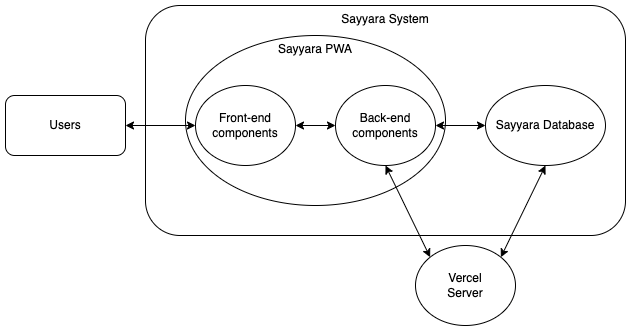
\includegraphics[width=\textwidth]{./diagrams/ContextDiagram.png}
	\caption{Context Diagram}
	\label{ContextDiagram}
\end{figure}

% \wss{Include a figure that show the System Context (showing the boundary between
% 	your system and the environment around it.)}

\section{Project Overview}

\subsection{Normal Behaviour}
Sayyara is an event-driven application which handles inputs from the intended users including:
vehicle owners, and independent auto repair shop owners and employees. The application will accept
various inputs through a variety of input forms and controls. Under normal behaviour where valid
inputs are entered and valid events are triggered, the application will: update the appropriate
local and global application states, trigger the corresponding side-effects, and/or update the
database accordingly.

Vehicle owners can search for auto repair shops and services; request quotes for service; book,
view, and manage service appointments and work orders. On the application, auto repair shop owners
will be able to manage a list of employees; manage a list of service types and corresponding
service appointment availabilities; manage store information such as location, hours of operation,
and contact information. Auto repair shop owners and employees will be able to view and manage
quotes, service appointments, and work orders.

\subsection{Undesired Event Handling}

Undesired events will be handled both client-side and server-side.

On the client-side, if an unexpected event arises or the application enters a bad state, the
application will reset to a safe state. For example, if a user attempts to access a route that they
are not authorized to access, they will be either redirected to an appropriate route, prompted to
login, or an error page will be displayed with instructions to return to the home page. Input forms
will also include input validation to ensure only properly formed data is handled. If the user
attempts to input invalid data, the form field will reset and form submission will be blocked. The
user will be prompted to enter a valid input value in the form field. Similarly, various user
actions and inputs that may pose cause that the application to enter an undesirable state will be
validated before updating the application state.

On the server-side, each API will return a response with the appropriate error status code and
message. Subsequently, the client will have logic to gracefully handle unsuccessful responses and
status codes, preventing the system from entering an undesirable state. Inputs will also be
validated on the server-side by parsing the input data using defined schemas. This will ensure data
integrity and prevents the undesirable data from entering the workflows or database.

\subsection{Component Diagram}

The Authentication Module is responsible for ensuring users have the appropriate permissions to
access resources and modules to perform specific actions. The Authentication Module is responsible
for handling authentication for requests between the client and server, and providing mechanisms
for authorizing access to requests resources. The Authentication Module will ensure that any
actions and interactions between modules are authorized based on the user and their permissions.
The Shop Module is responsible for handling requests associated with any shop entity, including
handling requests for shop creation, update, and look up. The Quotes Module is responsible for
handling requests and interactions for quotes, including the live chat module. The Appointments
Module is responsible for handling any appointment creations, appointment status updates,
appointment cancellations, and appointment edits. The Work Orders Module is responsible for
handling requests regarding the work order of a service, including creating the work order and
updating the work order. The Users Module is responsible for handling user account related requests
such as retrieving user data and user account creation for the shop owner, employee, and customer.
The Employee Management Module is responsible for handling employee requests such as getting all
employees in a shop and updating the employee account status to suspend employees. The Services
Module is responsible for handling requests to create, update, delete services and parts used for
each service. The Database Driver Module is responsible for providing a standard interface for
communication between the application and the database management system (DBMS). The database
driver module acts as a mediator between the application and the DBMS, and provides mechanisms for
the application to interact with the database.

\begin{figure}[H]
	\centering
	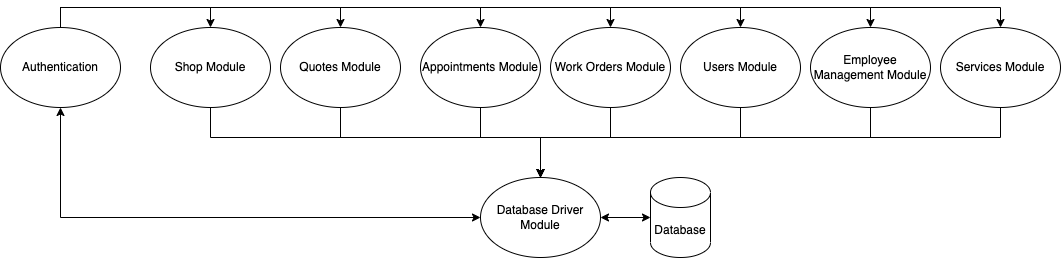
\includegraphics[width=\textwidth]{./diagrams/component-diagram.png}
	\caption{Component Diagram}
	\label{ComponentDiagram}
\end{figure}

\subsection{Connection Between Requirements and Design} \label{SecConnection}

% \wss{The intention of this section is to document decisions that are made
% 	``between'' the requirements and the design.  To satisfy some requirements,
% 	design decisions need to be made.  Rather than make these decisions implicit,
% 	they are explicitly recorded here.  For instance, if a program has security
% 	requirements, a specific design decision may be made to satisfy those
% 	requirements with a password.}

The following table shows the connections between the requirements stated in the SRS
\url{https://github.com/arkinmodi/project-sayyara/blob/main/docs/SRS/SRS.pdf} and our design
decisions to implement the requirements. The requirements in the table will refer to the
requirement number as stated in the SRS.

\begin{table}[H]
	\centering
	\caption{Connection Between Requirements and Design}
	\vspace{5pt}
	\begin{tabular}{|p{0.3\textwidth}|p{0.6\textwidth}|}
		\hline
		\textbf{Requirement} & \textbf{Design Decision}                                                                                                                                                                                                    \\
		\hline
		BE4                  & A calendar dropdown is used to allow the user to view appointment dates                                                                                                                                                     \\
		\hline
		BE8, BE20            & The quotes, appointments are in a tab view for easy visibility                                                                                                                                                              \\
		\hline
		BE25                 & Employees are listed in a list view                                                                                                                                                                                         \\
		\hline
		BE32                 & Shops are listed in a list view, with tags showing information relevant to the filters (such as services provided and parts used)                                                                                           \\
		\hline
		LF1                  & Each screen has a desktop and mobile view so that it can adjust cleanly based on the user's screen size                                                                                                                     \\
		\hline
		SR1, SR2             & Separate views are created for each type of user, so that they have access to only information that the specific user needs. Each account is created with a unique user type, so that they can only access the correct view \\
		\hline
		LR1                  & Images and assets used are either created by the team or provided by the stakeholder                                                                                                                                        \\
		\hline
	\end{tabular}
\end{table}

\section{System Variables}
\subsection{Monitored Variables}
N/A

\subsection{Controlled Variables}
N/A

\subsection{Constants Variables}
N/A

\section{User Interfaces}

% \wss{Design of user interface for software and hardware.  Attach an appendix if
% 	needed. Drawings, Sketches, Figma}

\subsection{Home Page}

\begin{figure}[H]
	\centering
	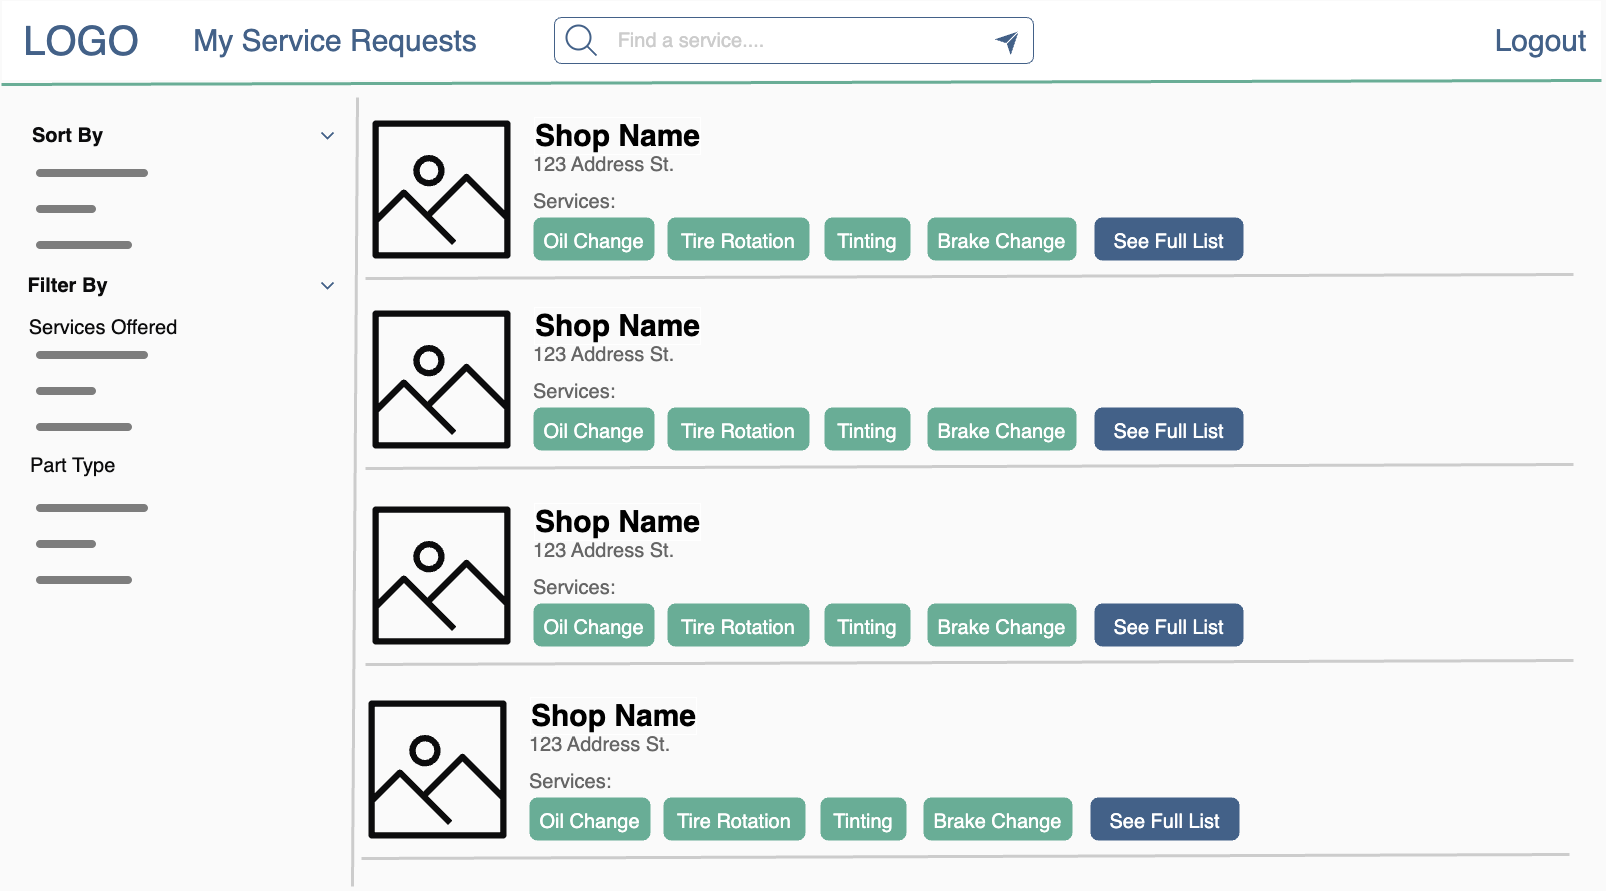
\includegraphics[width=\textwidth]{mockups/Home Page (Logged In) (Desktop).png}
	\caption{Home Page \textemdash{} Logged In (Desktop)}
\end{figure}

\begin{figure}[H]
	\centering
	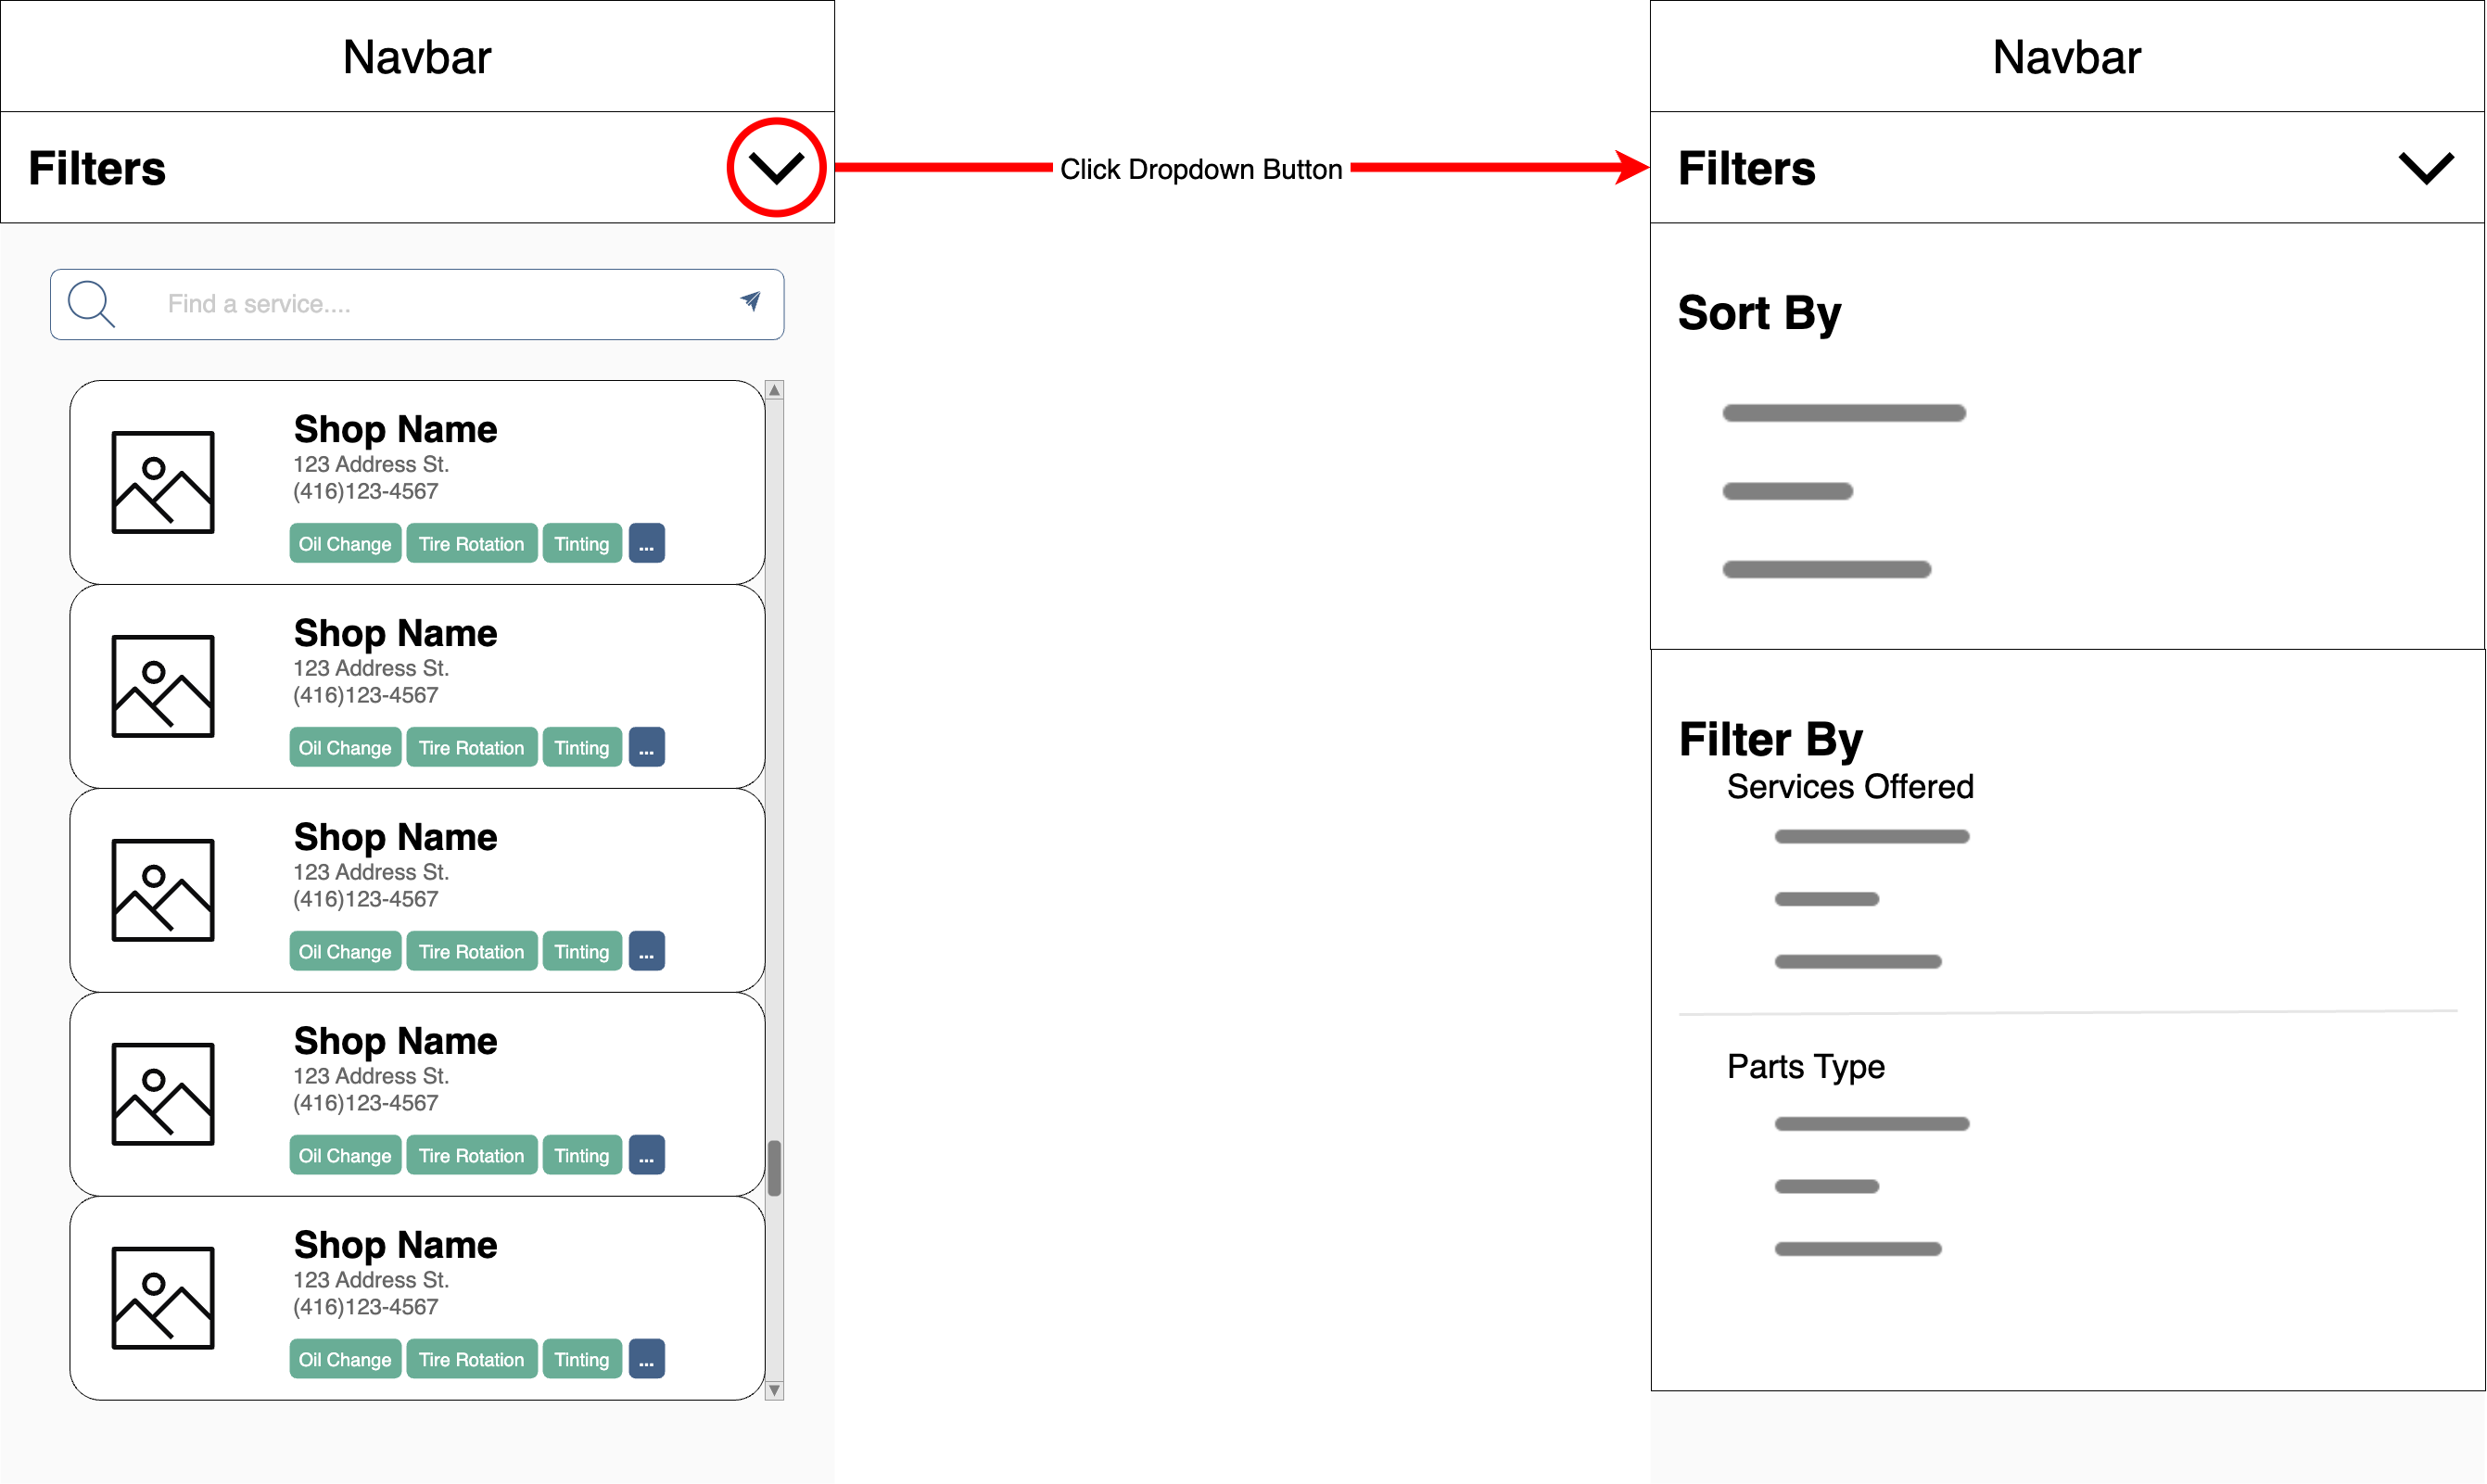
\includegraphics[width=\textwidth]{mockups/Home Page (Mobile).png}
	\caption{Home Page \textemdash{} Logged In (Mobile)}
\end{figure}

\subsection{Manage Shop Employees}

\begin{figure}[H]
	\centering
	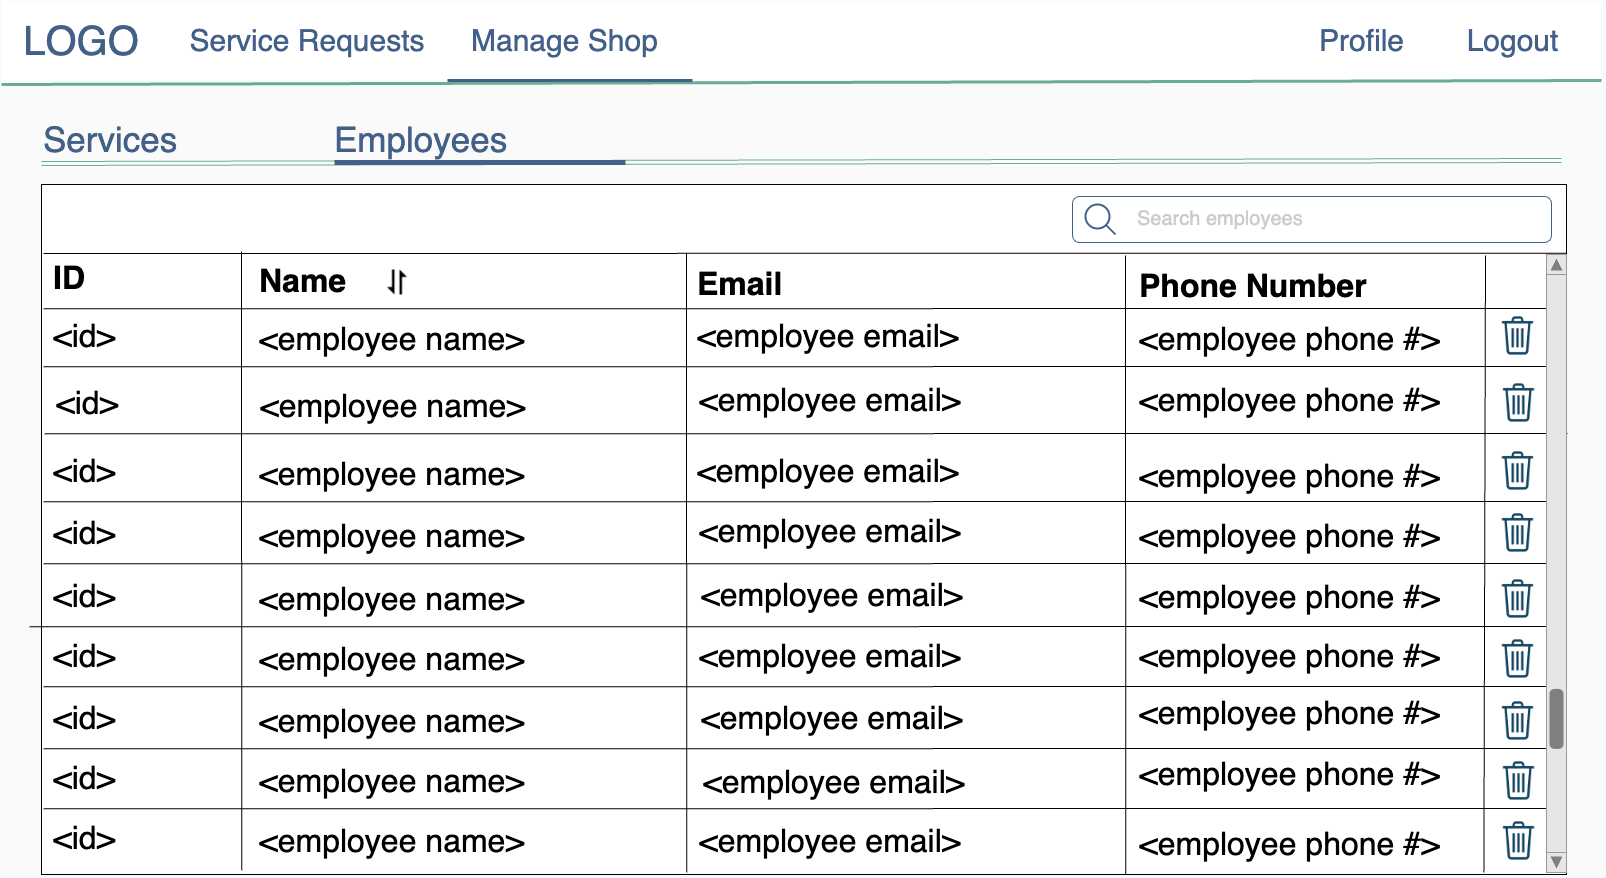
\includegraphics[width=\textwidth]{mockups/Manage Shop (Employees) (Desktop).png}
	\caption{Manage Shop \textemdash{} Employees (Desktop)}
\end{figure}

\begin{figure}[H]
	\centering
	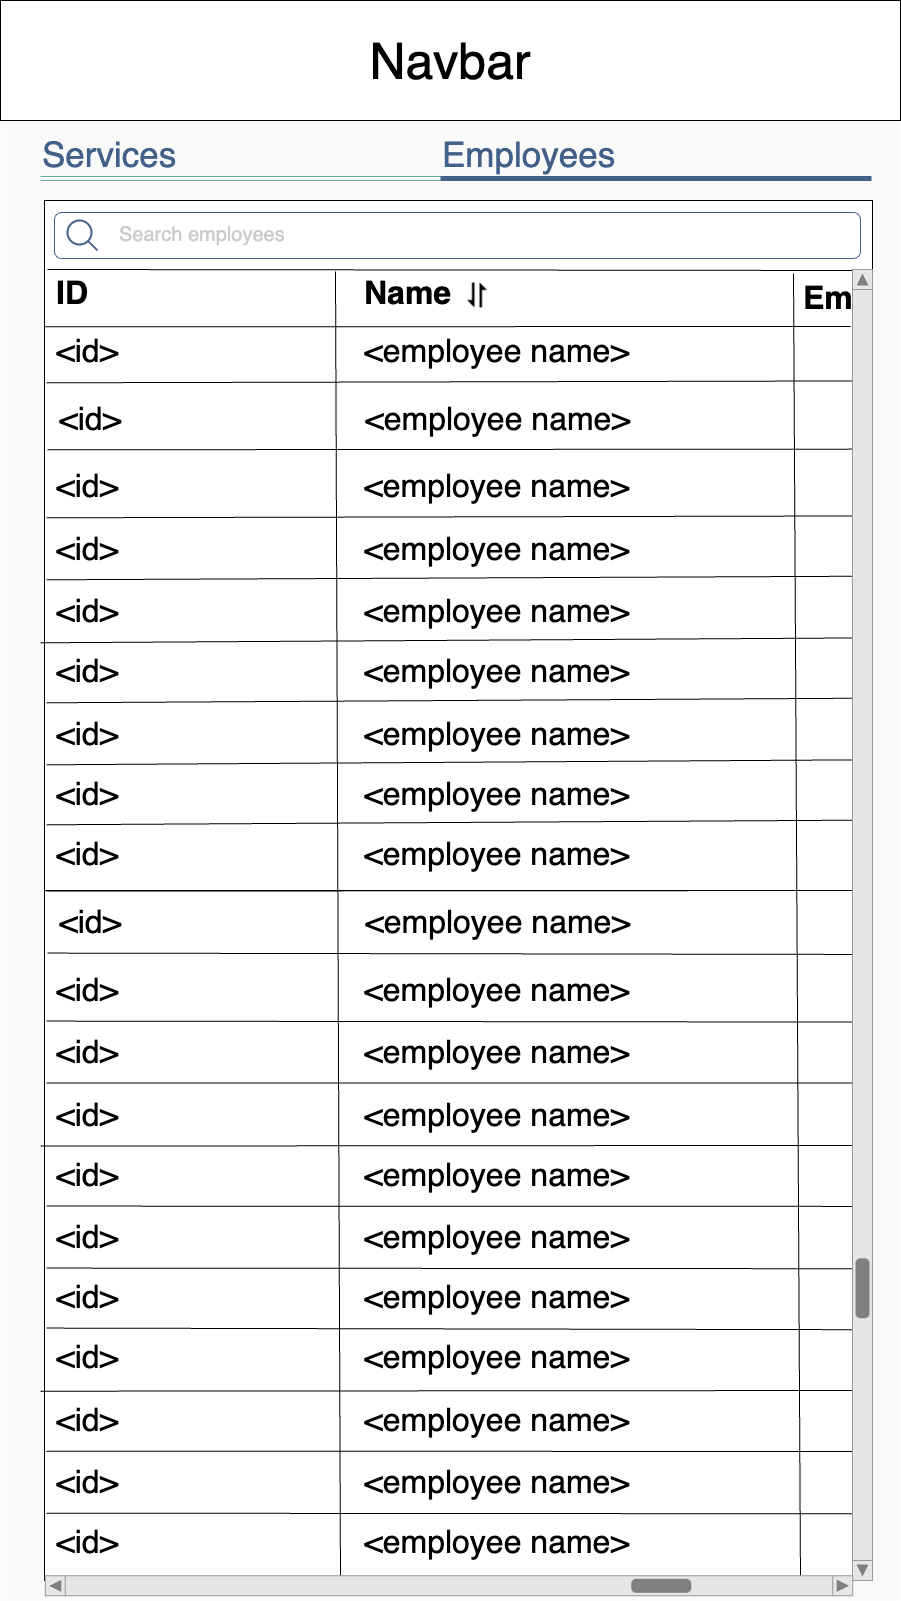
\includegraphics[width=0.5\textwidth]{mockups/Manage Shop (Employees) (Mobile).png}
	\caption{Manage Shop \textemdash{} Employees (Mobile)}
\end{figure}

\subsection{Manage Shop Details}

\begin{figure}[H]
	\centering
	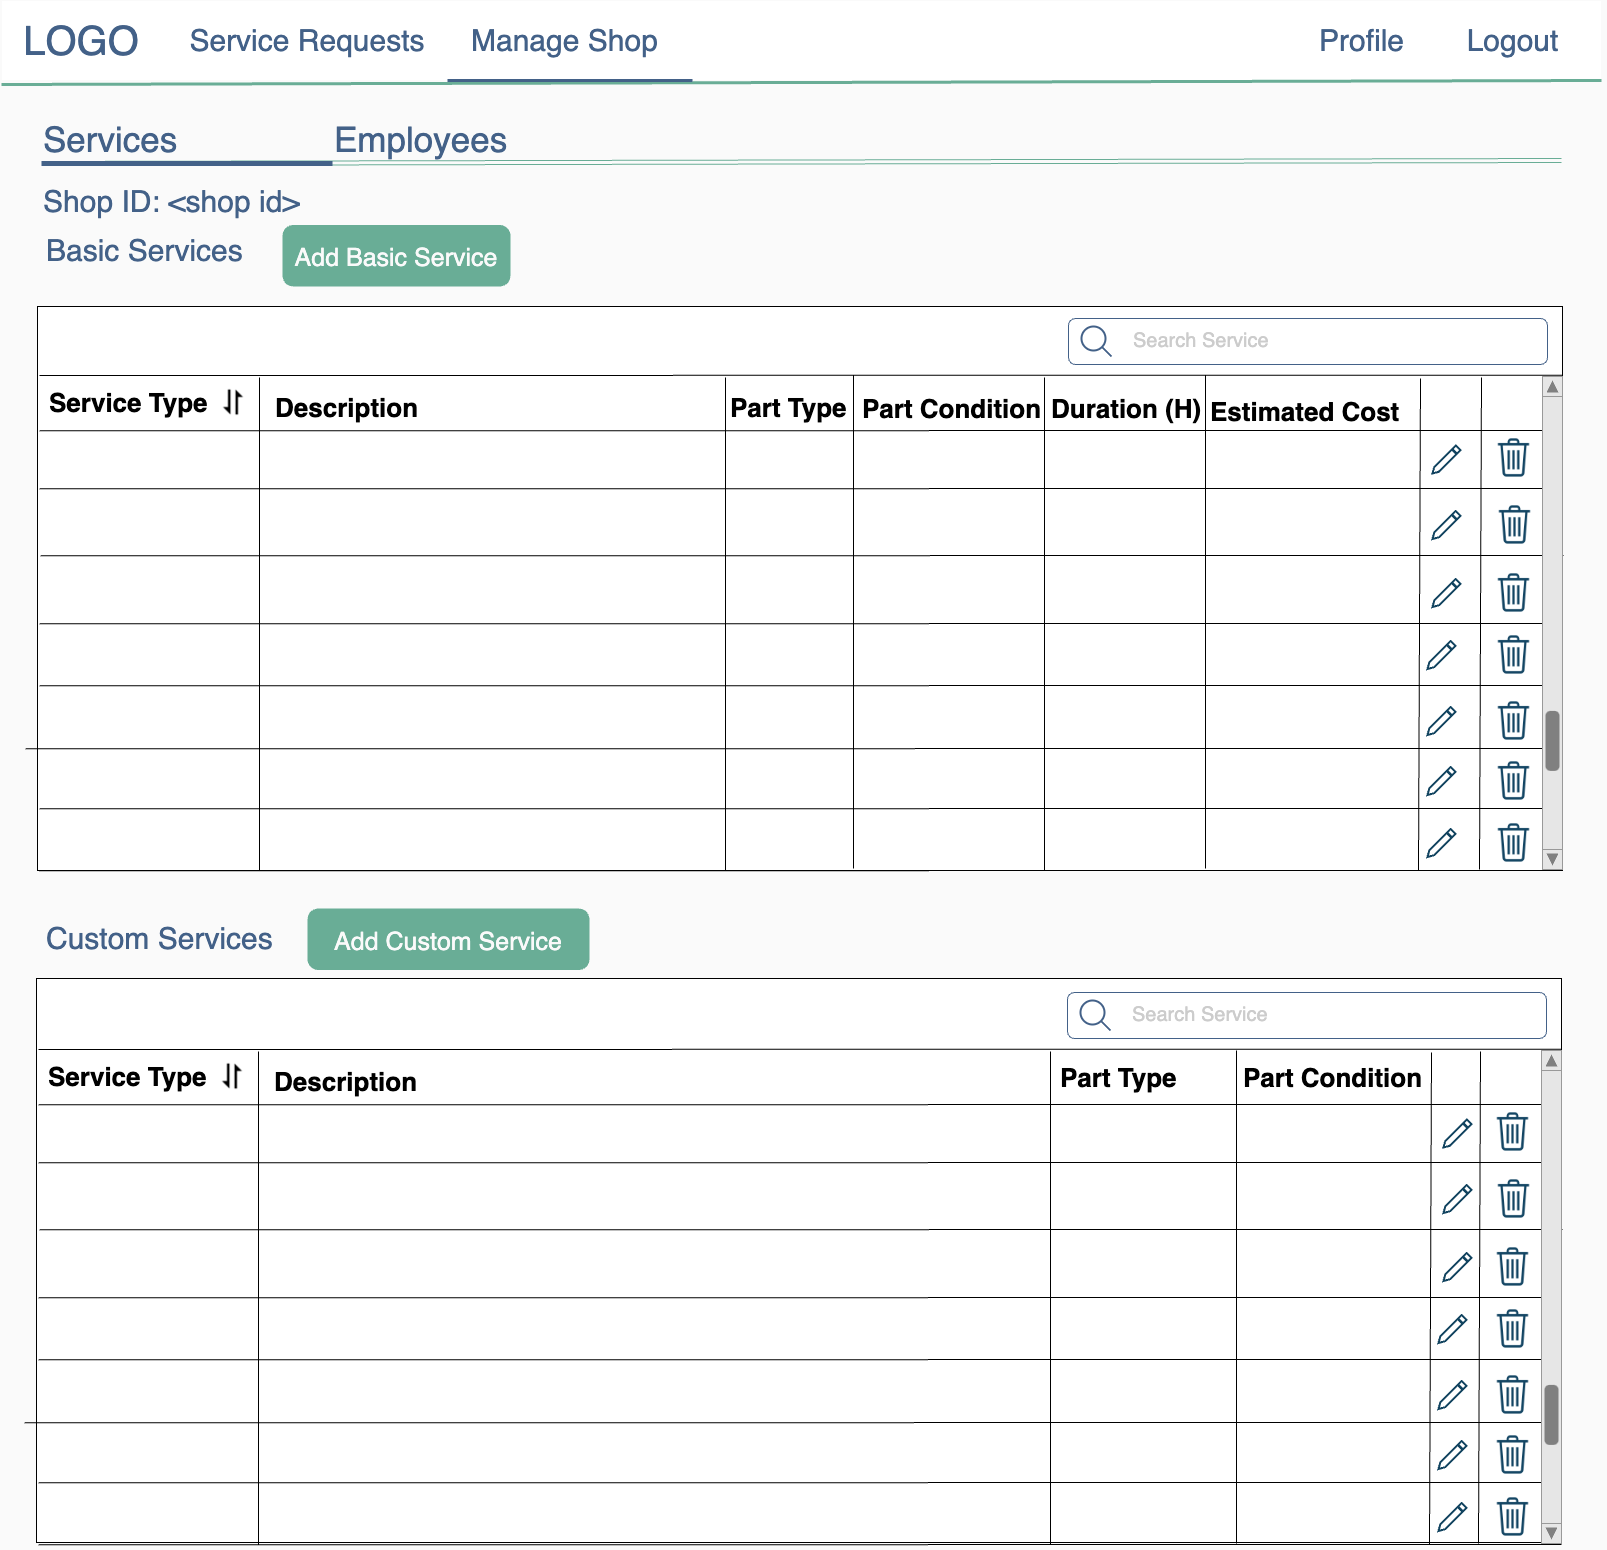
\includegraphics[width=\textwidth]{mockups/Manage Shop (Shop Settings) (Desktop).png}
	\caption{Manage Shop \textemdash{} Details (Desktop)}
\end{figure}

\begin{figure}[H]
	\centering
	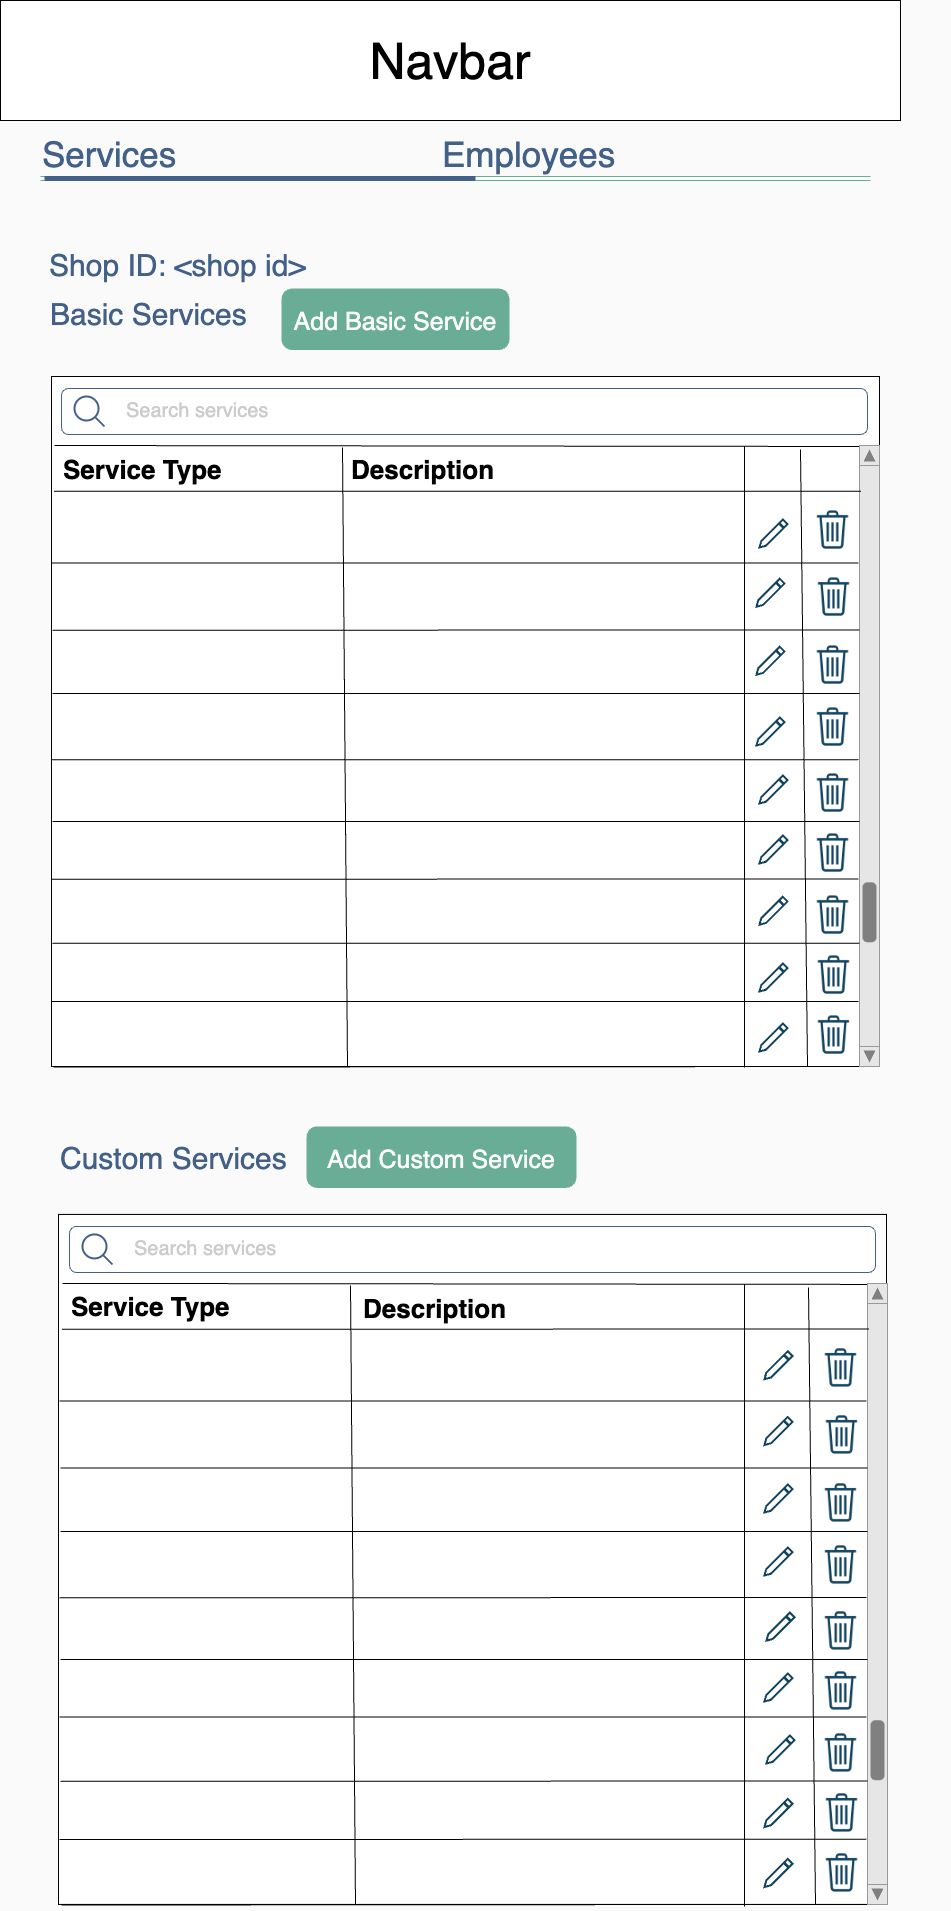
\includegraphics[width=0.5\textwidth]{mockups/Manage Shop (Shop Settings) (Mobile).png}
	\caption{Manage Shop \textemdash{} Details (Mobile)}
\end{figure}

\subsection{Shop Profile}

\begin{figure}[H]
	\centering
	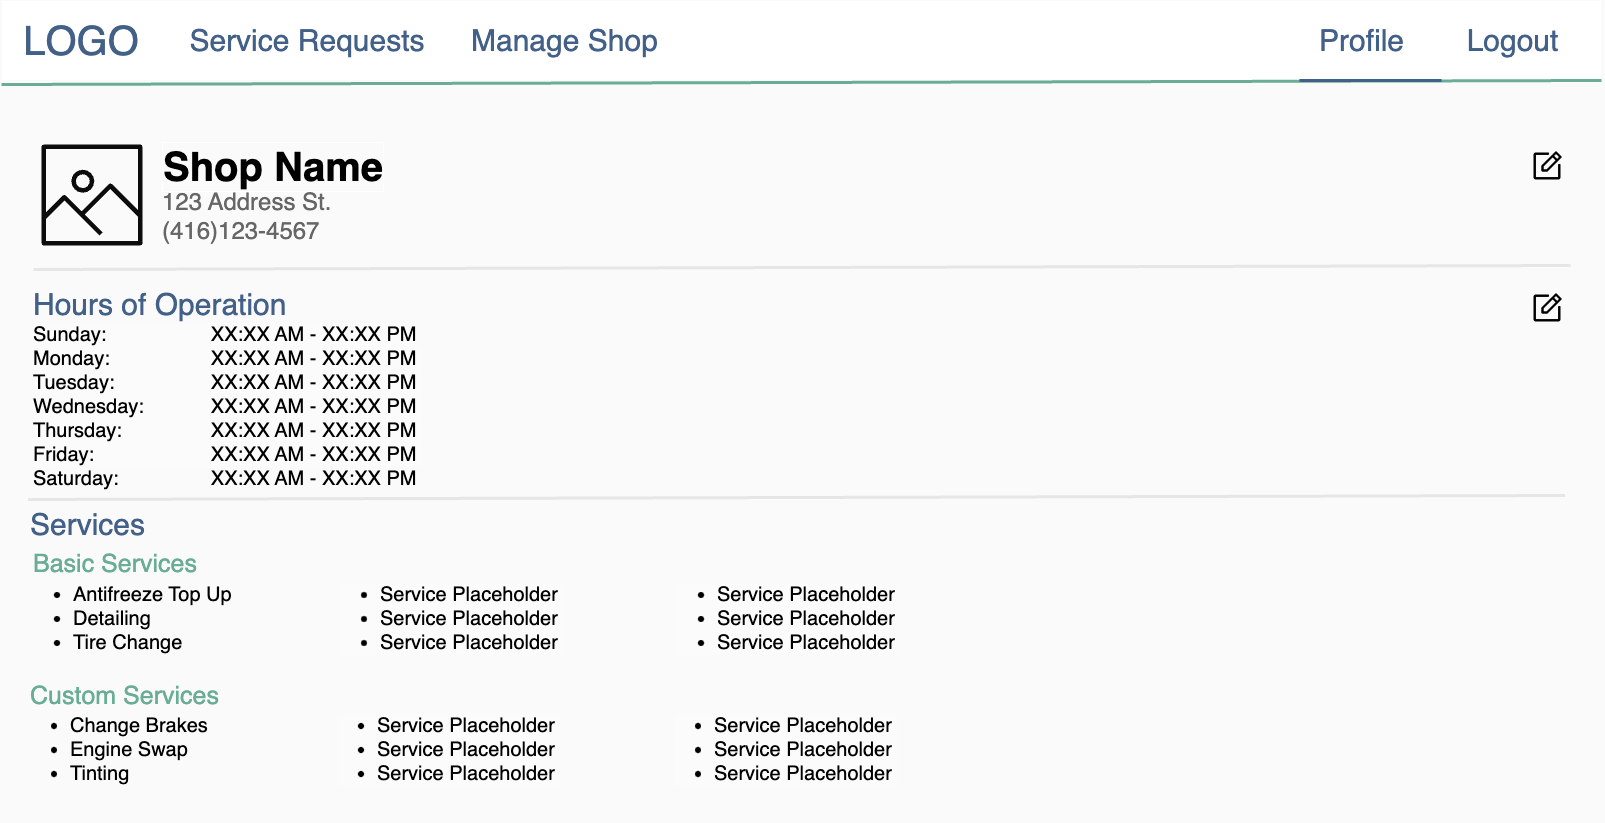
\includegraphics[width=\textwidth]{mockups/Shop Profile (Shop Owner) (Desktop).png}
	\caption{Shop Profile \textemdash{} Shop Owner (Desktop)}
\end{figure}

\begin{figure}[H]
	\centering
	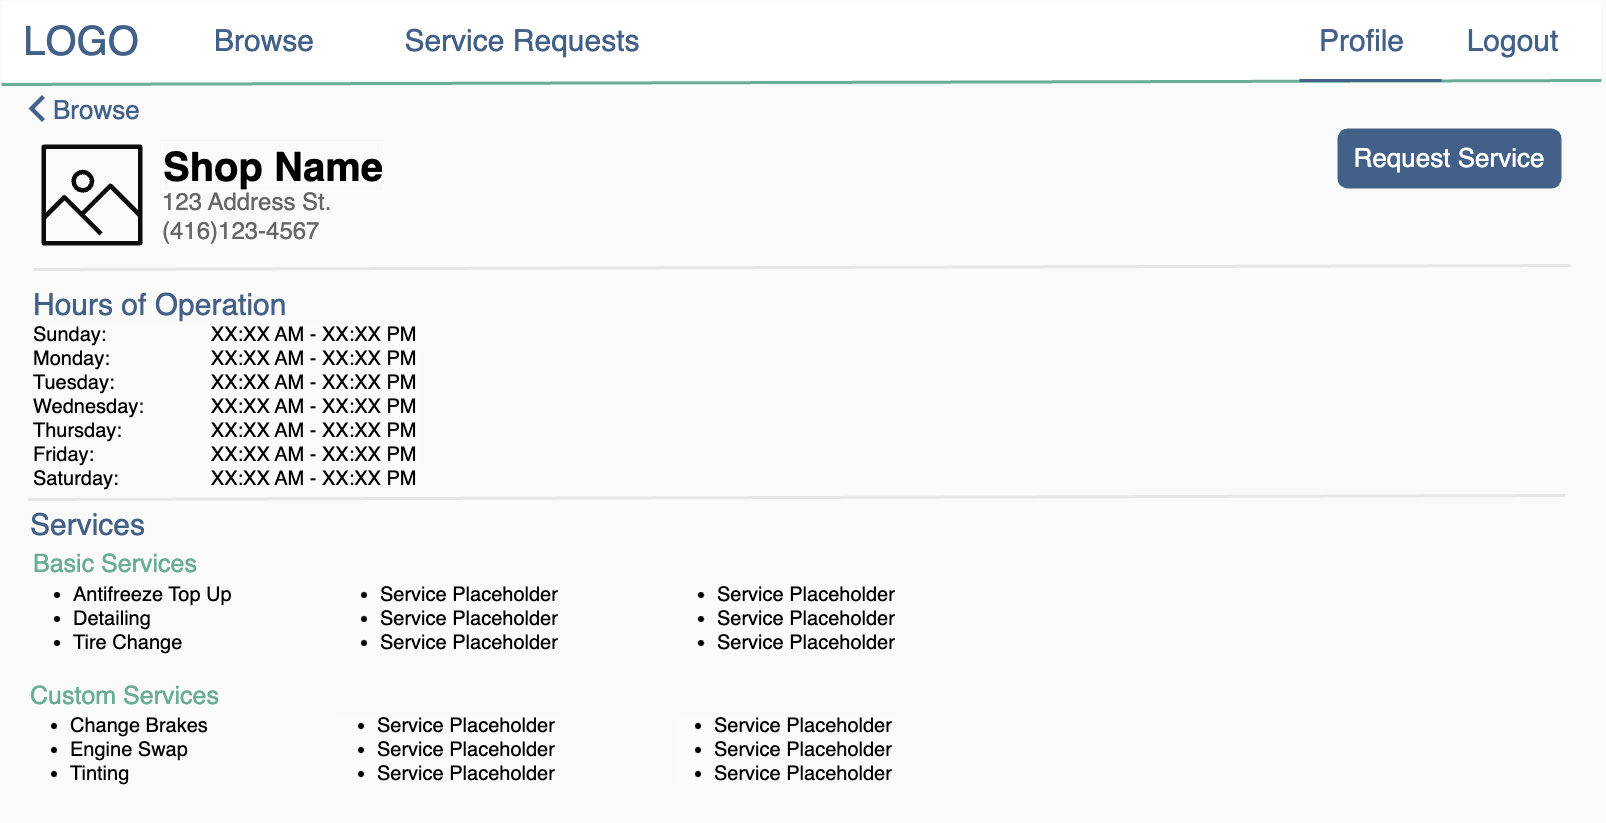
\includegraphics[width=\textwidth]{mockups/Shop Profile (Vehicle Owner) (Desktop).png}
	\caption{Shop Profile \textemdash{} Vehicle Owner (Desktop)}
\end{figure}

\begin{figure}[H]
	\centering
	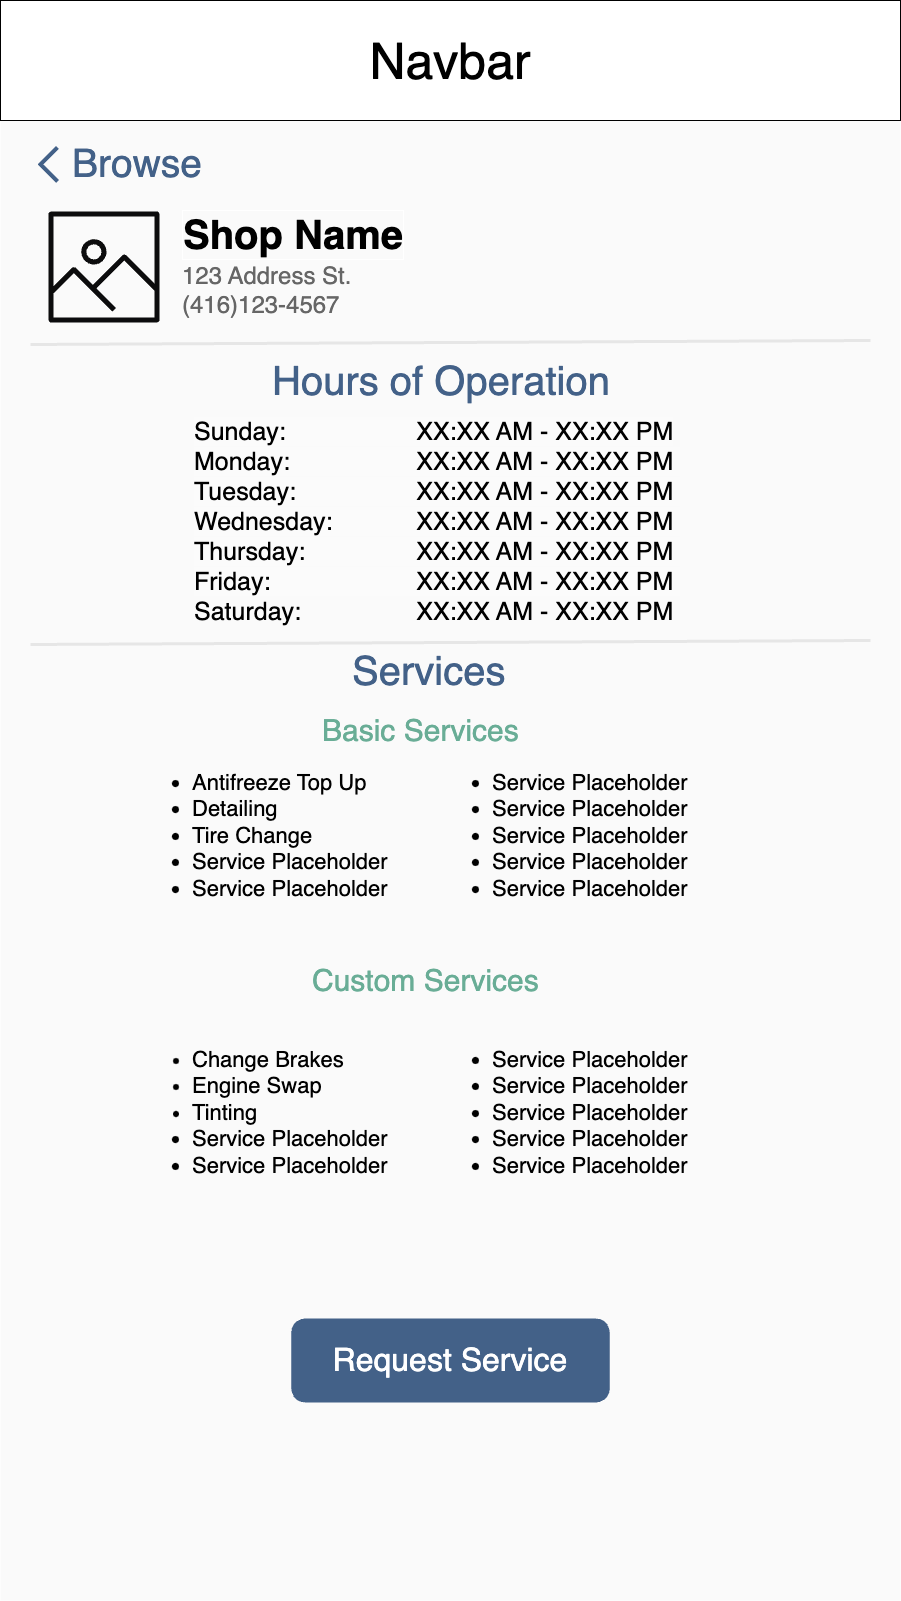
\includegraphics[width=0.5\textwidth]{mockups/Shop Profile (Mobile).png}
	\caption{Shop Profile (Mobile)}
\end{figure}

\subsection{Add Service to Shop}

\begin{figure}[H]
	\centering
	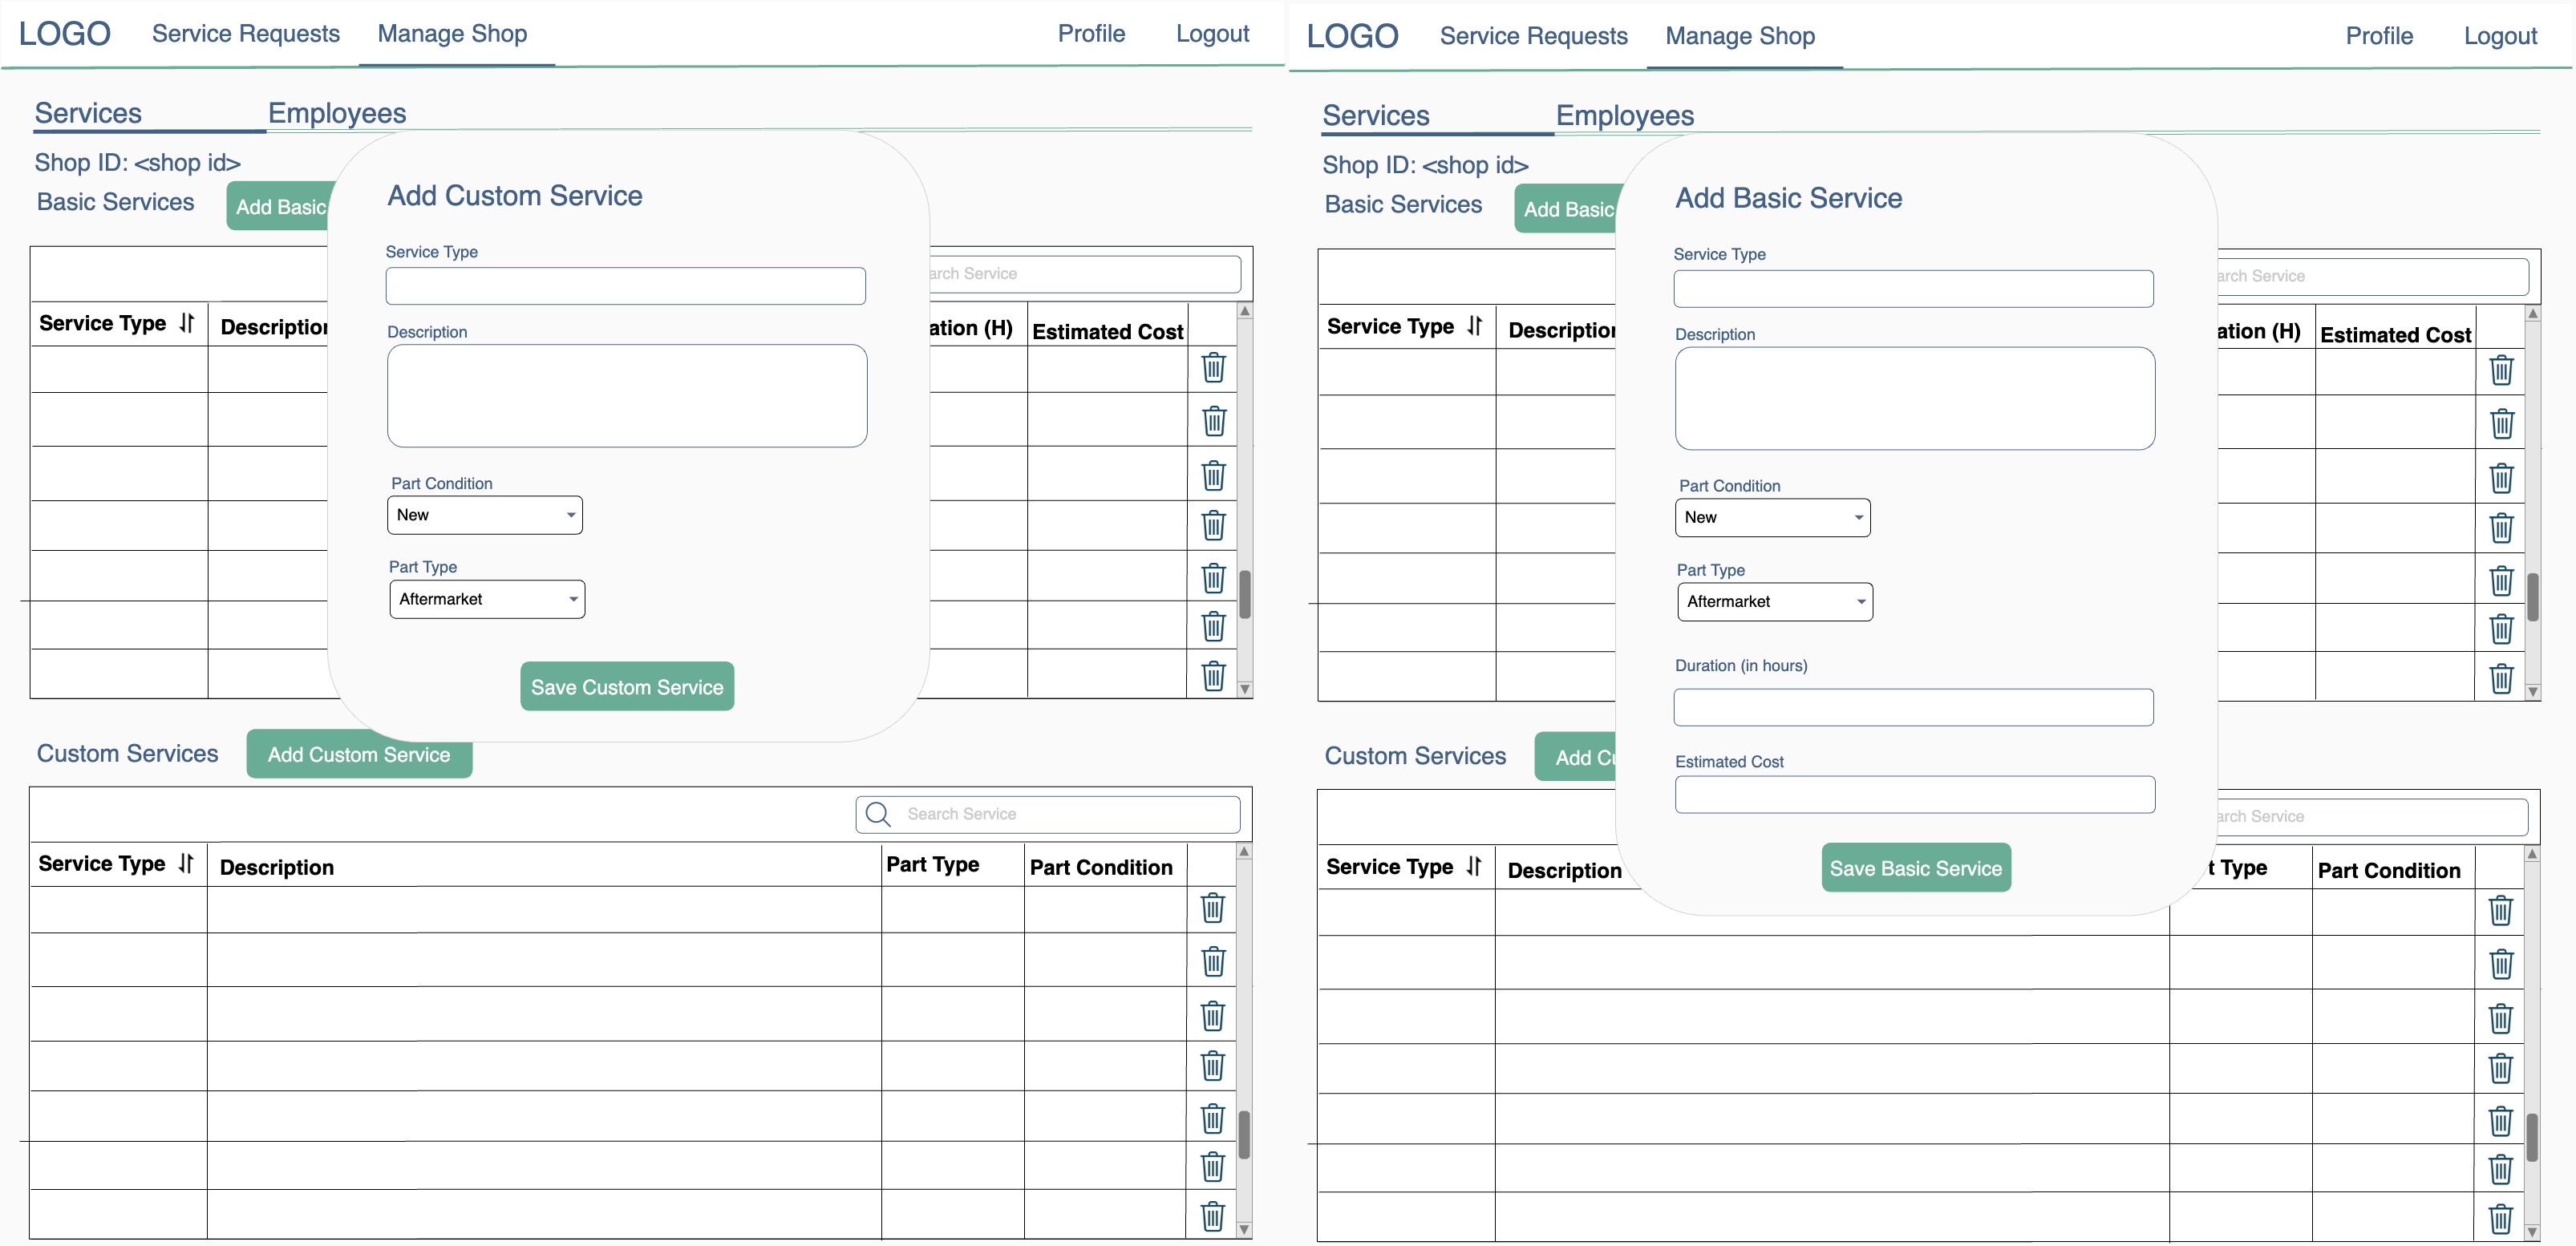
\includegraphics[width=\textwidth]{mockups/Service Form (Shop Settings) (Desktop).png}
	\caption{Add Service to Shop (Desktop)}
\end{figure}

\begin{figure}[H]
	\centering
	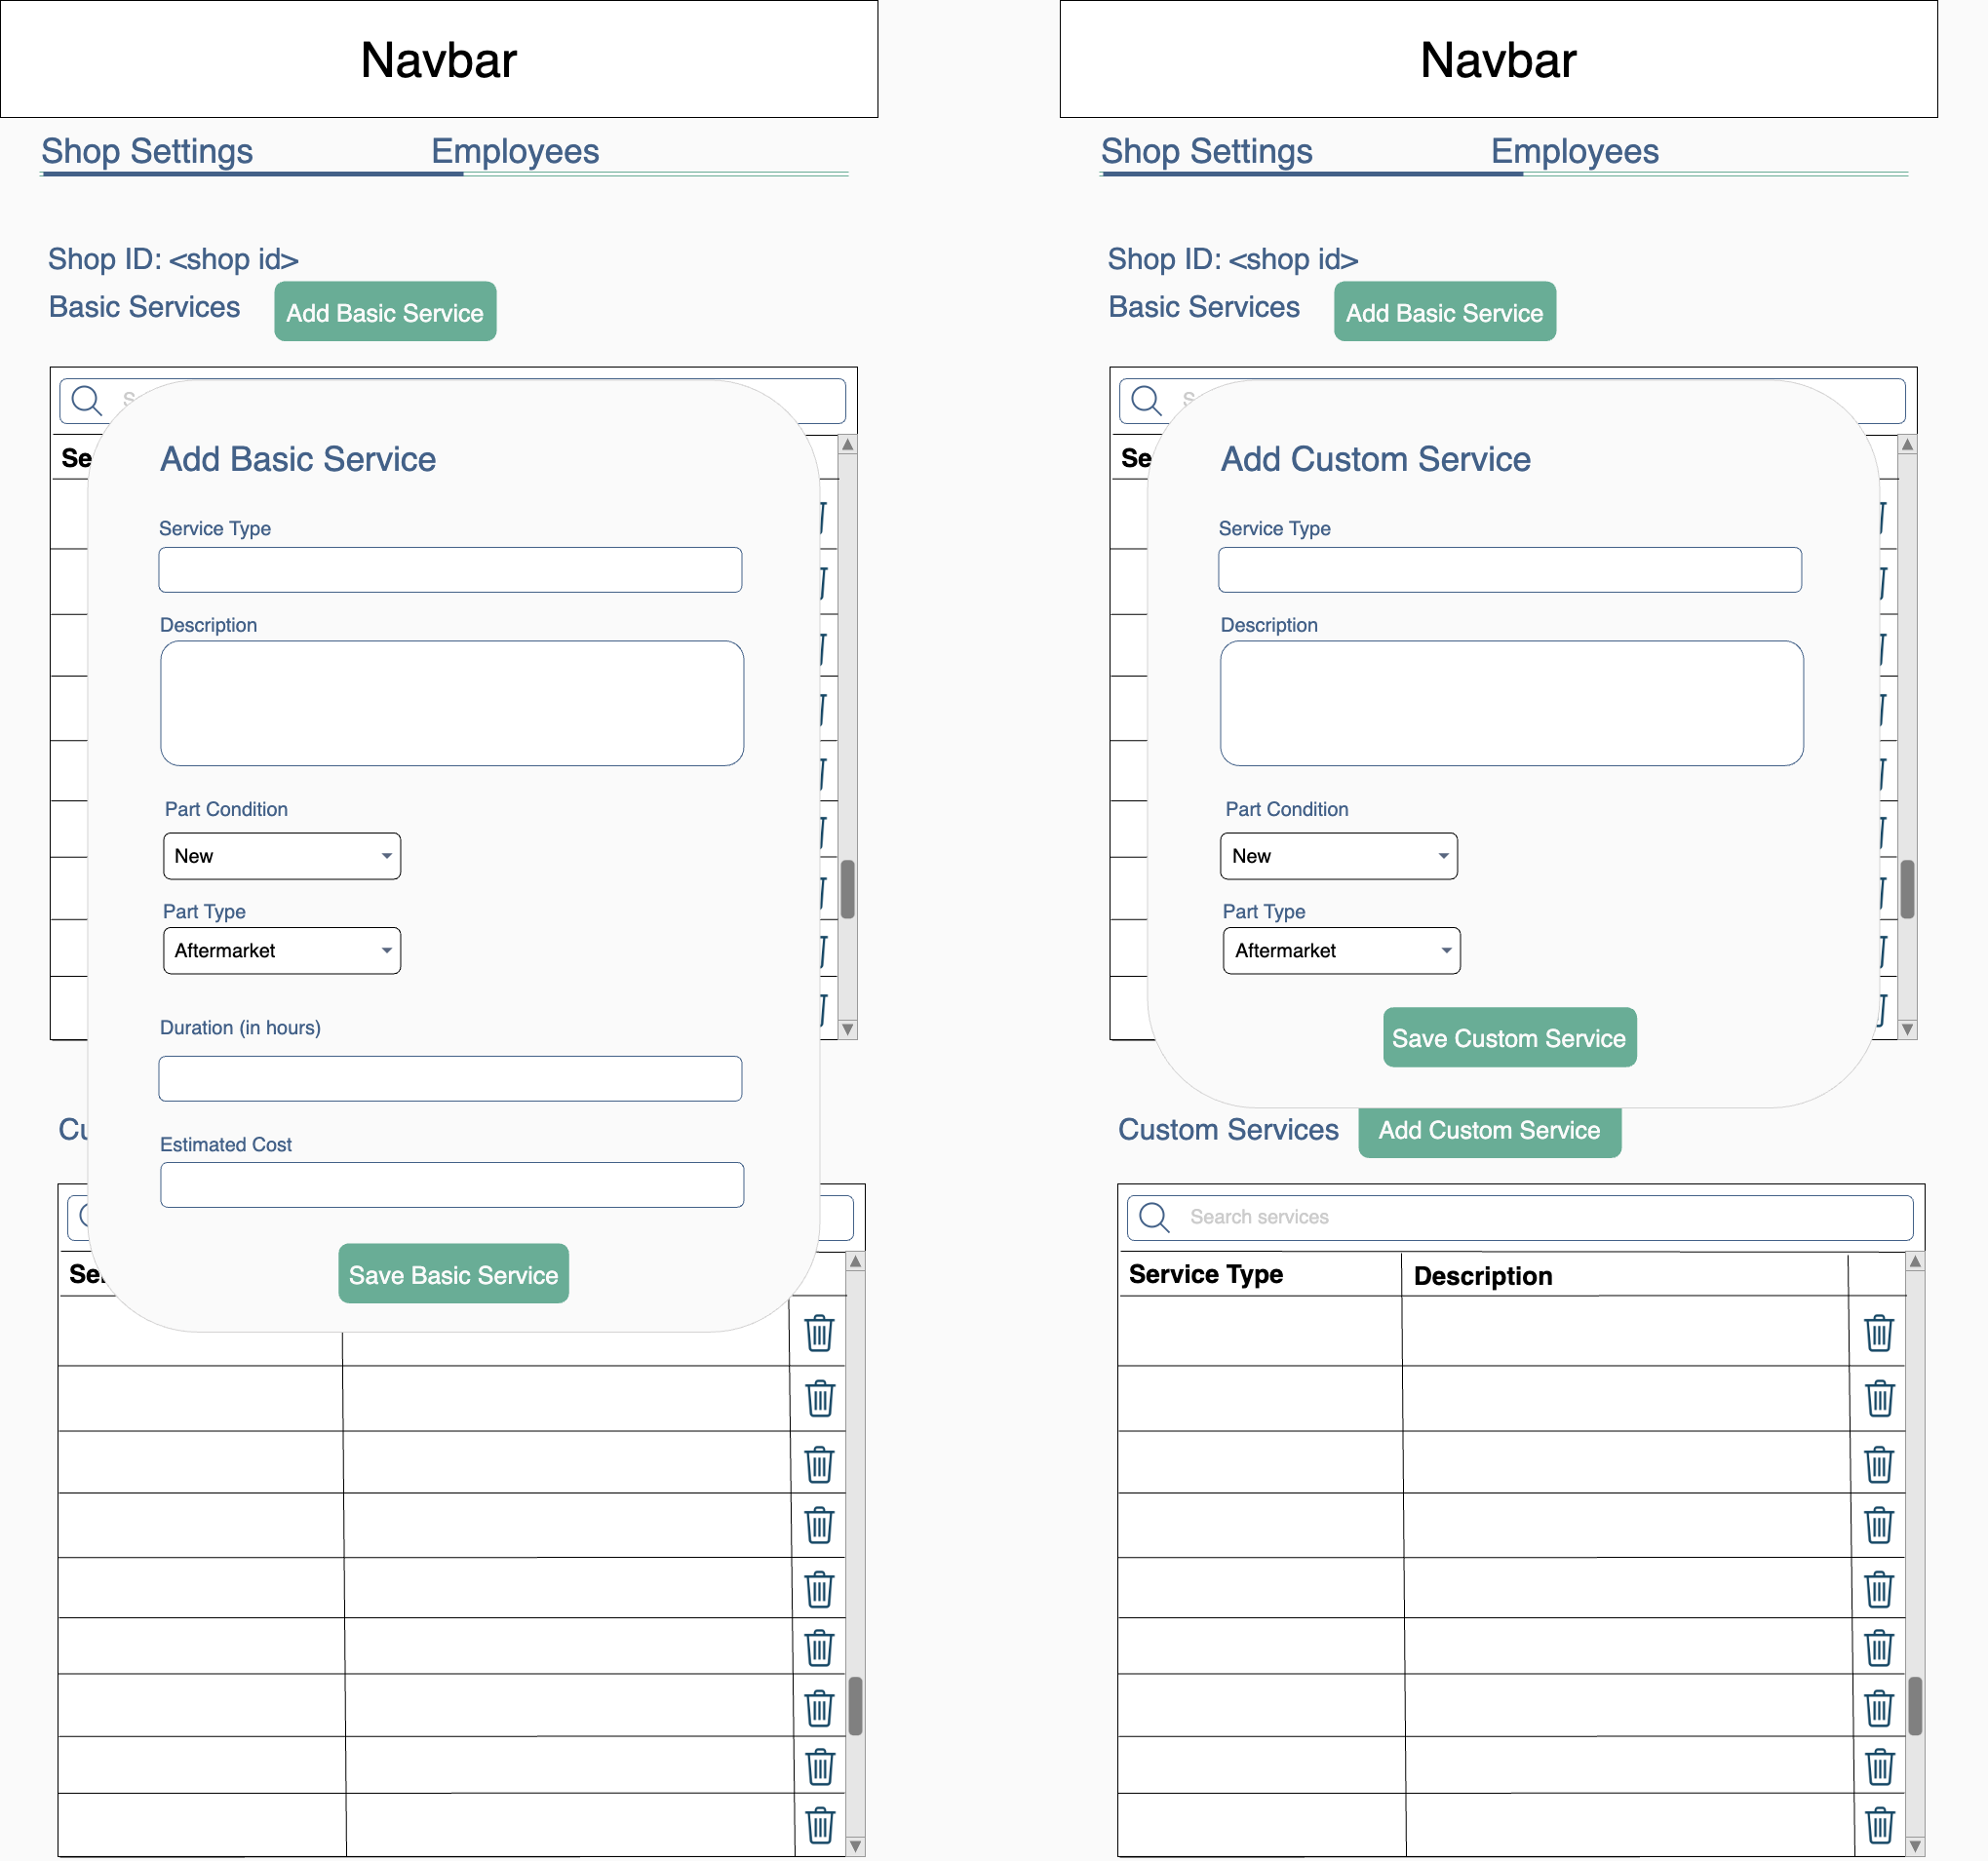
\includegraphics[width=\textwidth]{mockups/Service Form (Shop Settings) (Mobile).png}
	\caption{Add Service to Shop (Mobile)}
\end{figure}

\subsection{Shop Owner/Employee Registration}

\begin{figure}[H]
	\centering
	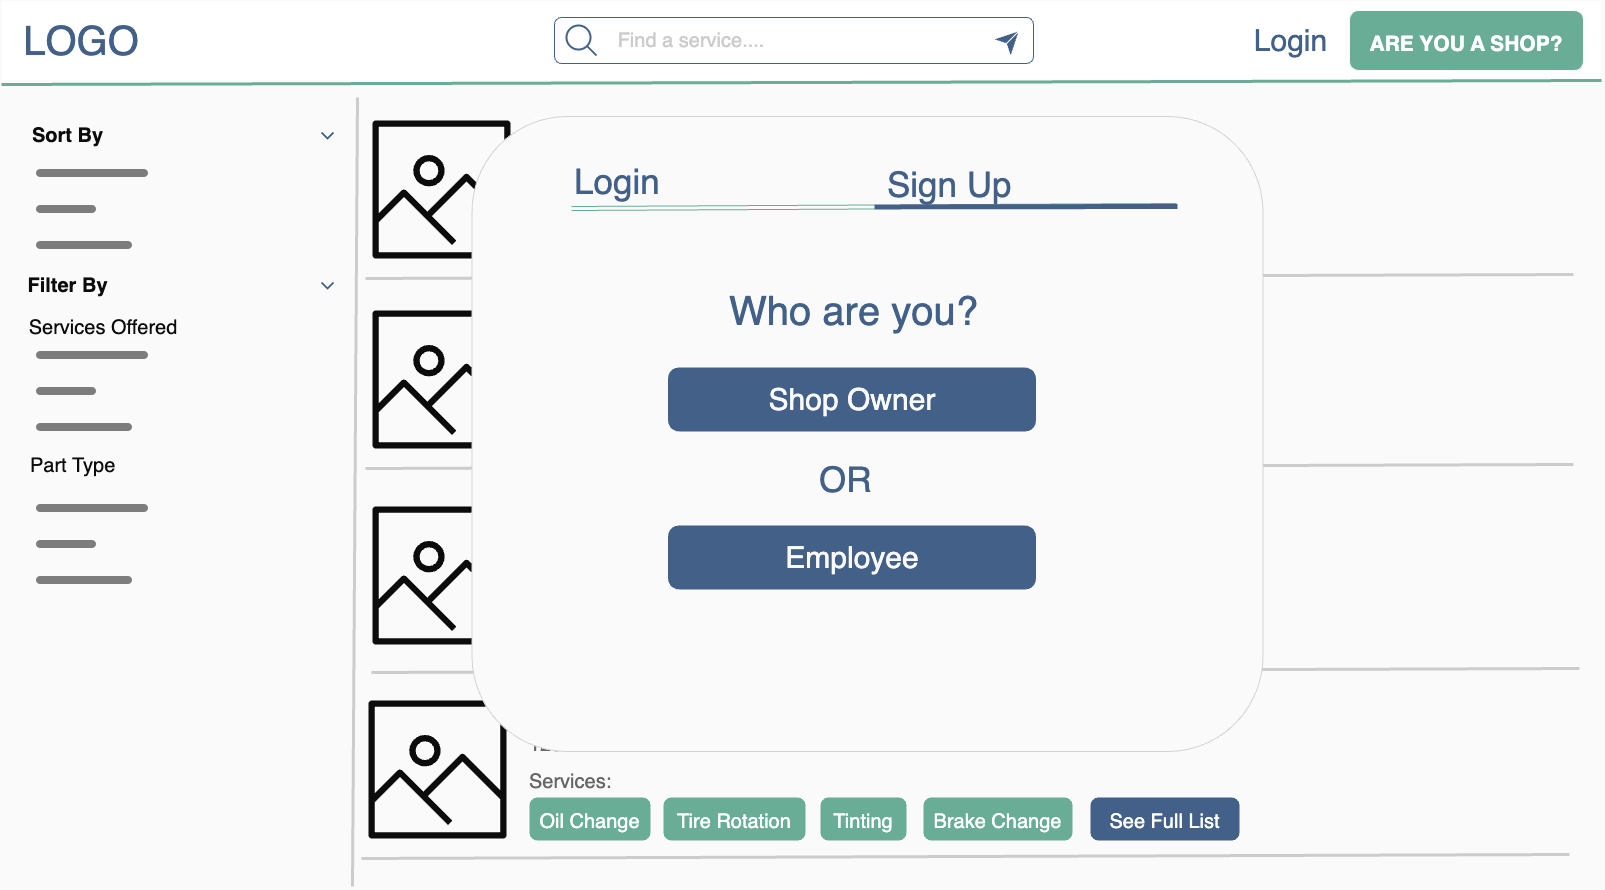
\includegraphics[width=\textwidth]{mockups/Shop Sign Up (Desktop).png}
	\caption{Shop Owner/Employee Registration \textemdash{} Part 1 (Desktop)}
\end{figure}

\begin{figure}[H]
	\centering
	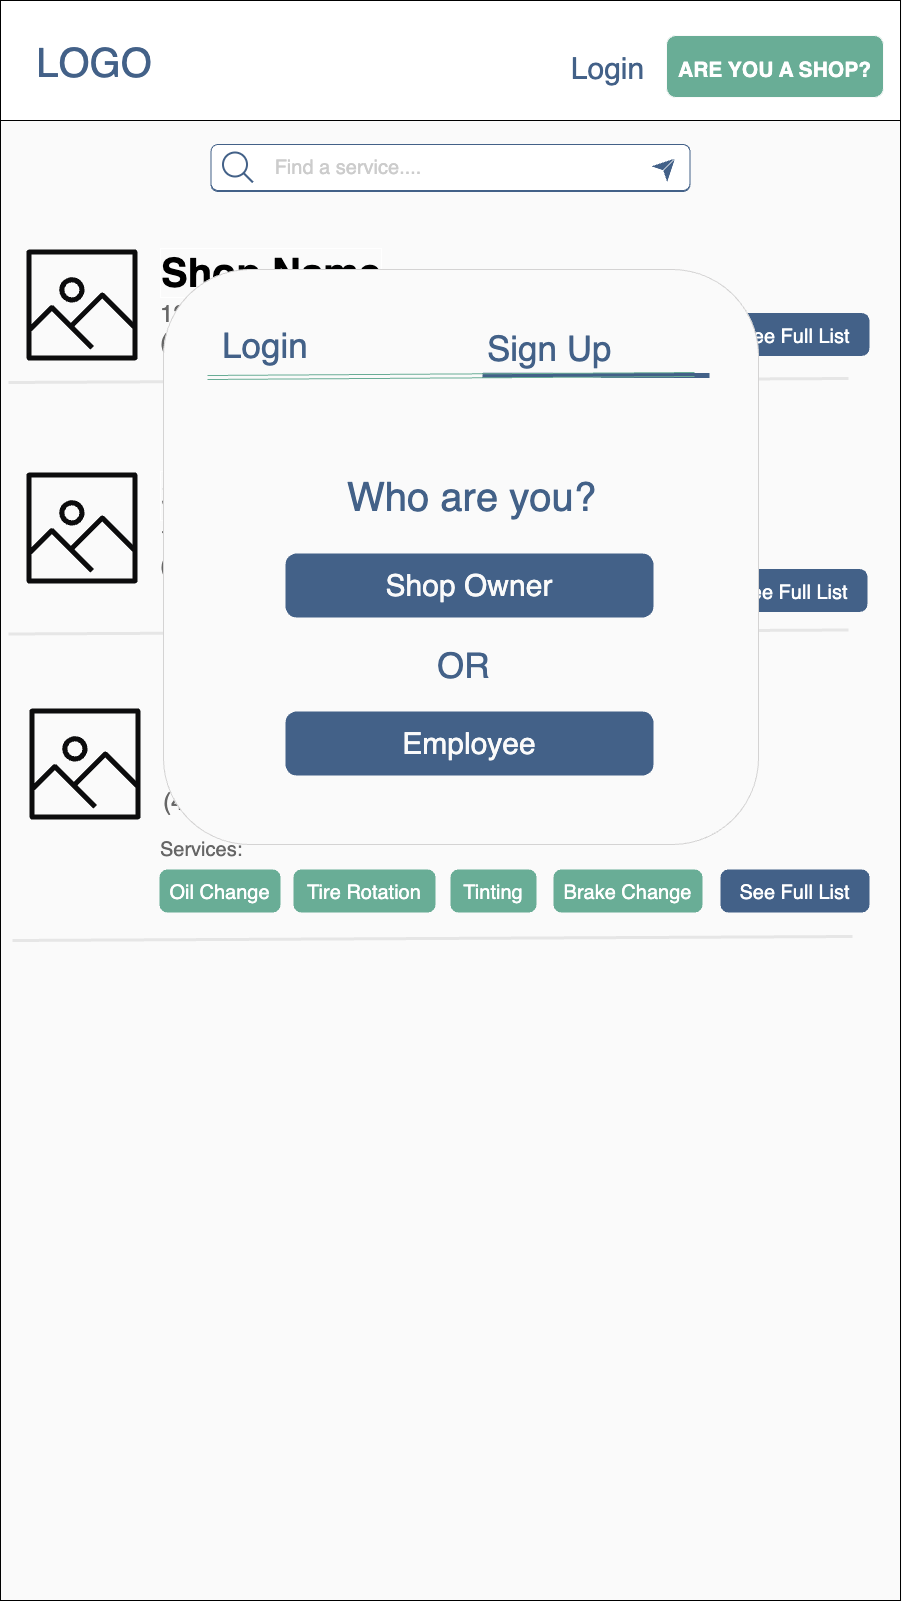
\includegraphics[width=0.5\textwidth]{mockups/Shop Sign Up (Mobile).png}
	\caption{Shop Owner/Employee Registration \textemdash{} Part 1 (Mobile)}
\end{figure}

\begin{figure}[H]
	\centering
	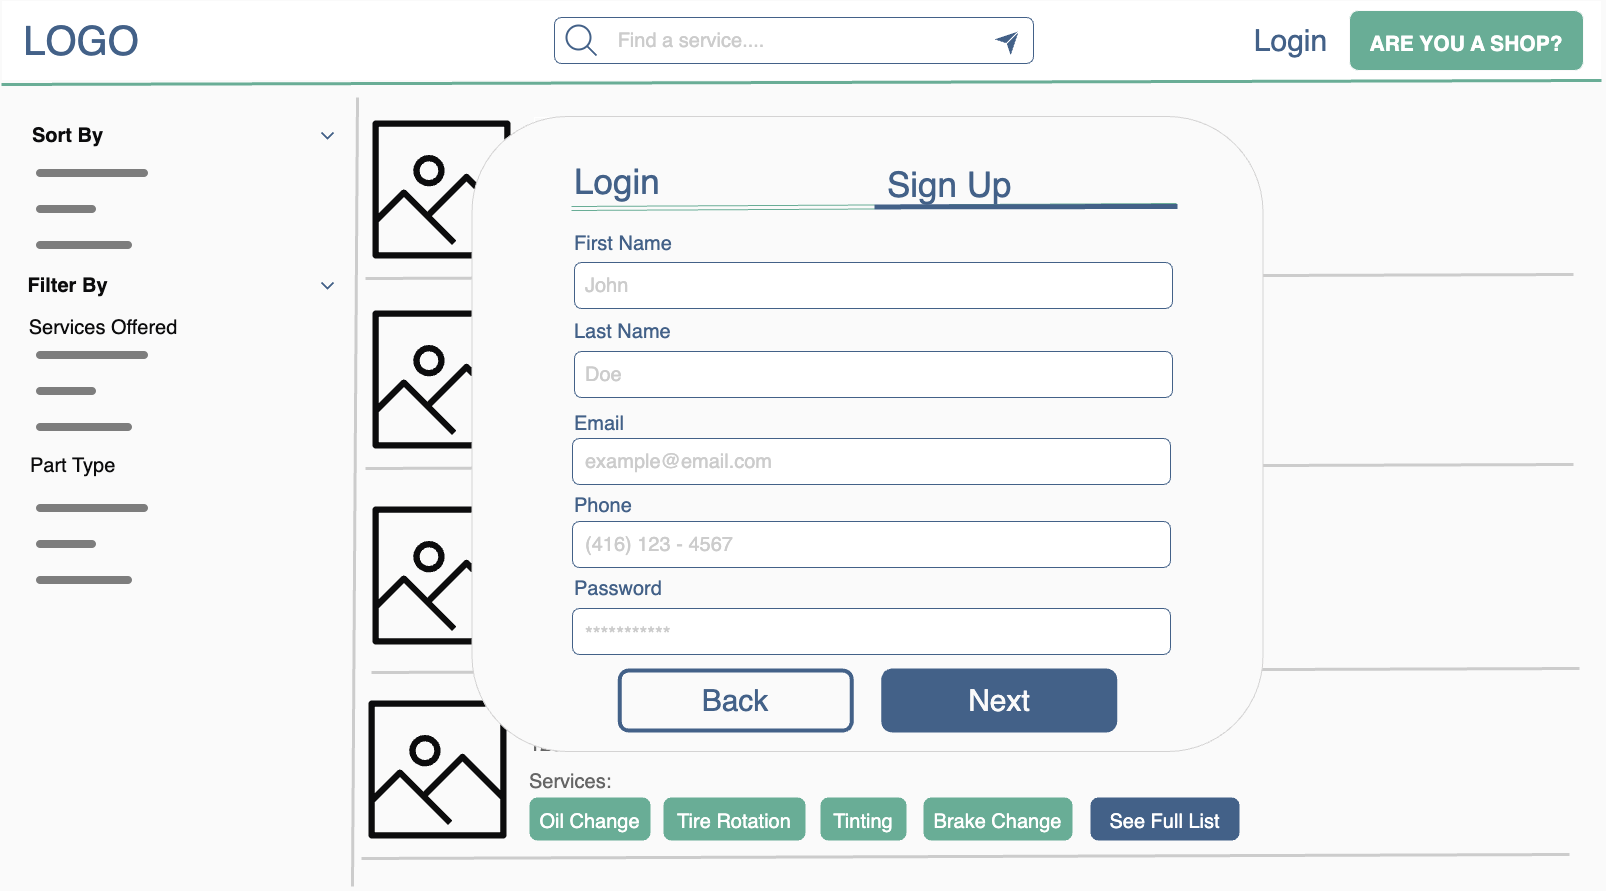
\includegraphics[width=\textwidth]{mockups/Shop Sign Up (Part 1) (Desktop).png}
	\caption{Shop Owner/Employee Registration \textemdash{} Part 2 (Desktop)}
\end{figure}

\begin{figure}[H]
	\centering
	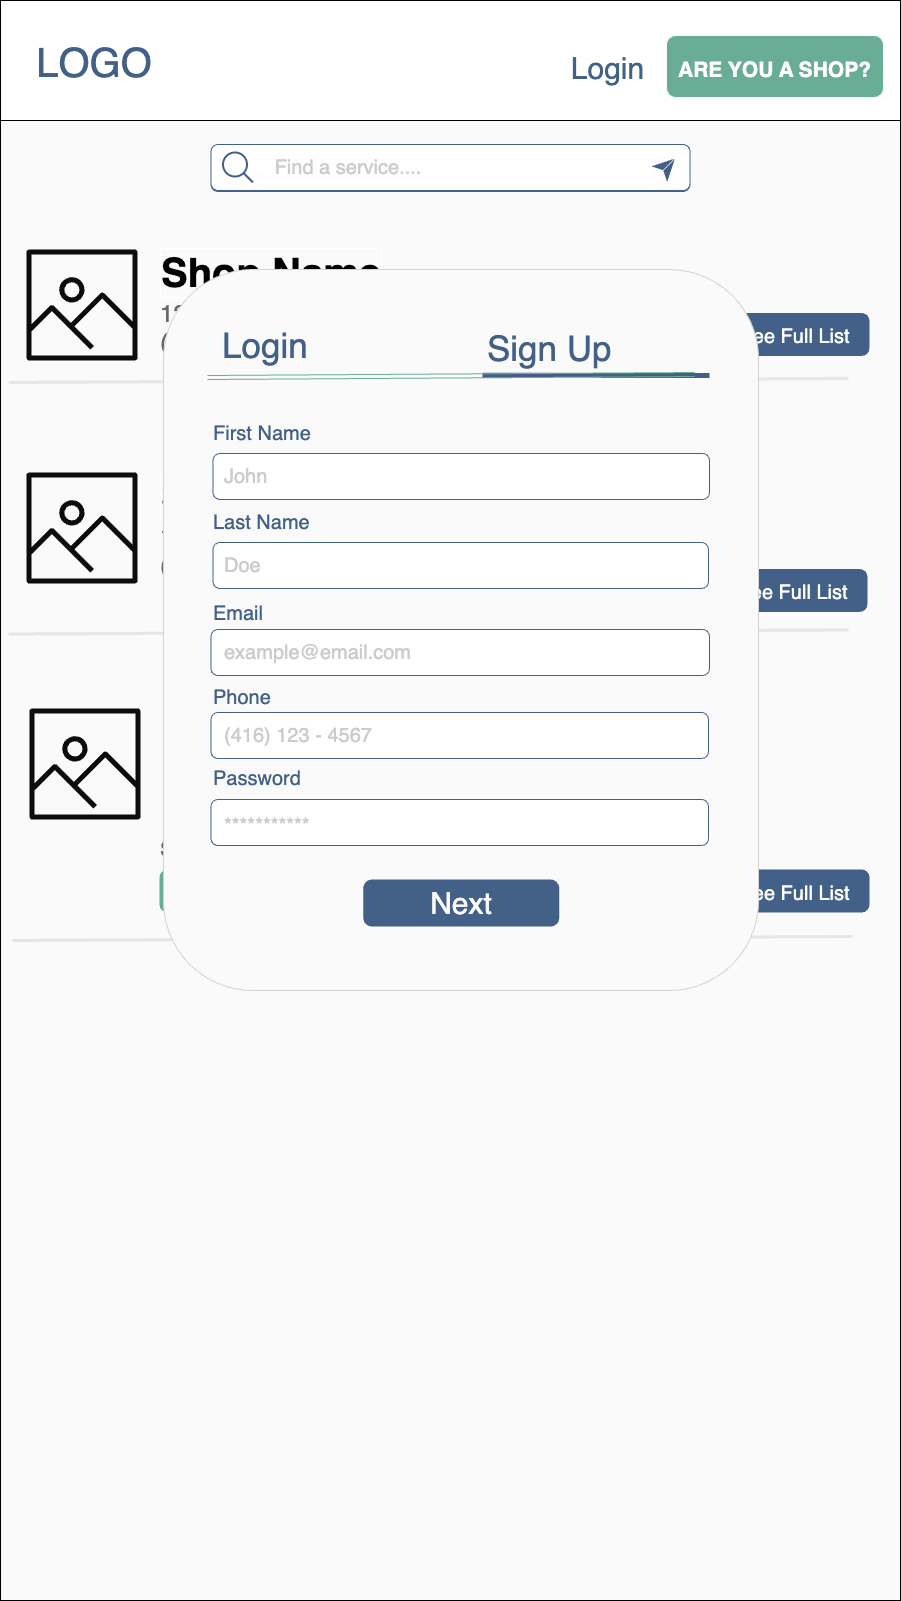
\includegraphics[width=0.5\textwidth]{mockups/Shop Sign Up (Part 1) (Mobile).png}
	\caption{Shop Owner/Employee Registration \textemdash{} Part 2 (Mobile)}
\end{figure}

\begin{figure}[H]
	\centering
	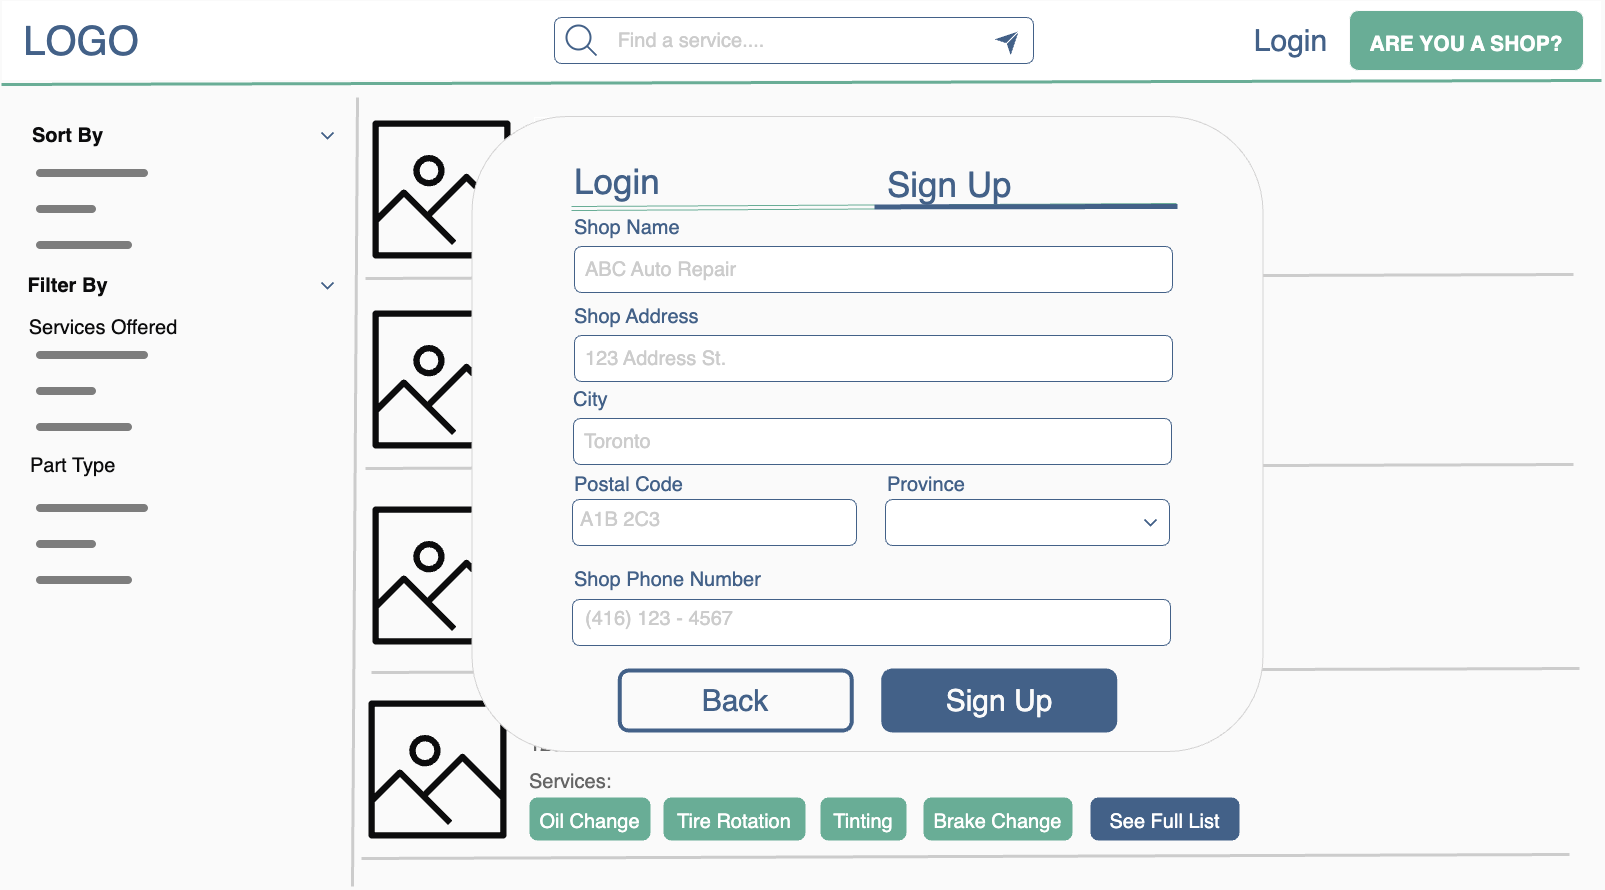
\includegraphics[width=\textwidth]{mockups/Shop Owner Signup (Part 2) (Desktop).png}
	\caption{Shop Owner Registration \textemdash{} Part 3 (Desktop)}
\end{figure}

\begin{figure}[H]
	\centering
	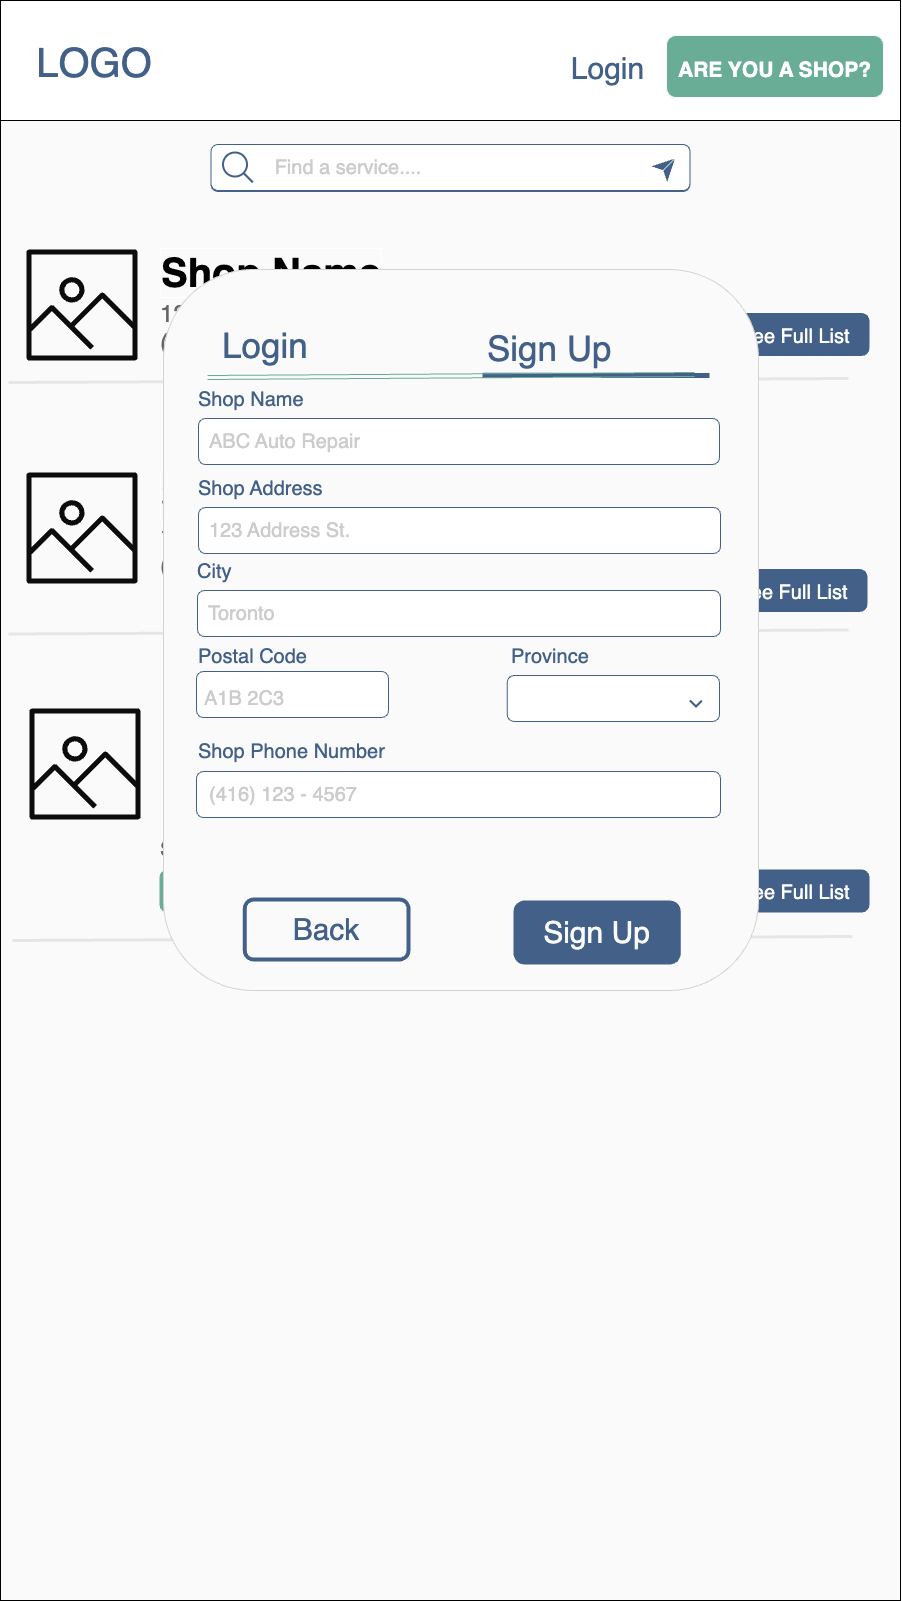
\includegraphics[width=0.5\textwidth]{mockups/Shop Owner Signup (Part 2) (Mobile).png}
	\caption{Shop Owner Registration \textemdash{} Part 3 (Mobile)}
\end{figure}

\begin{figure}[H]
	\centering
	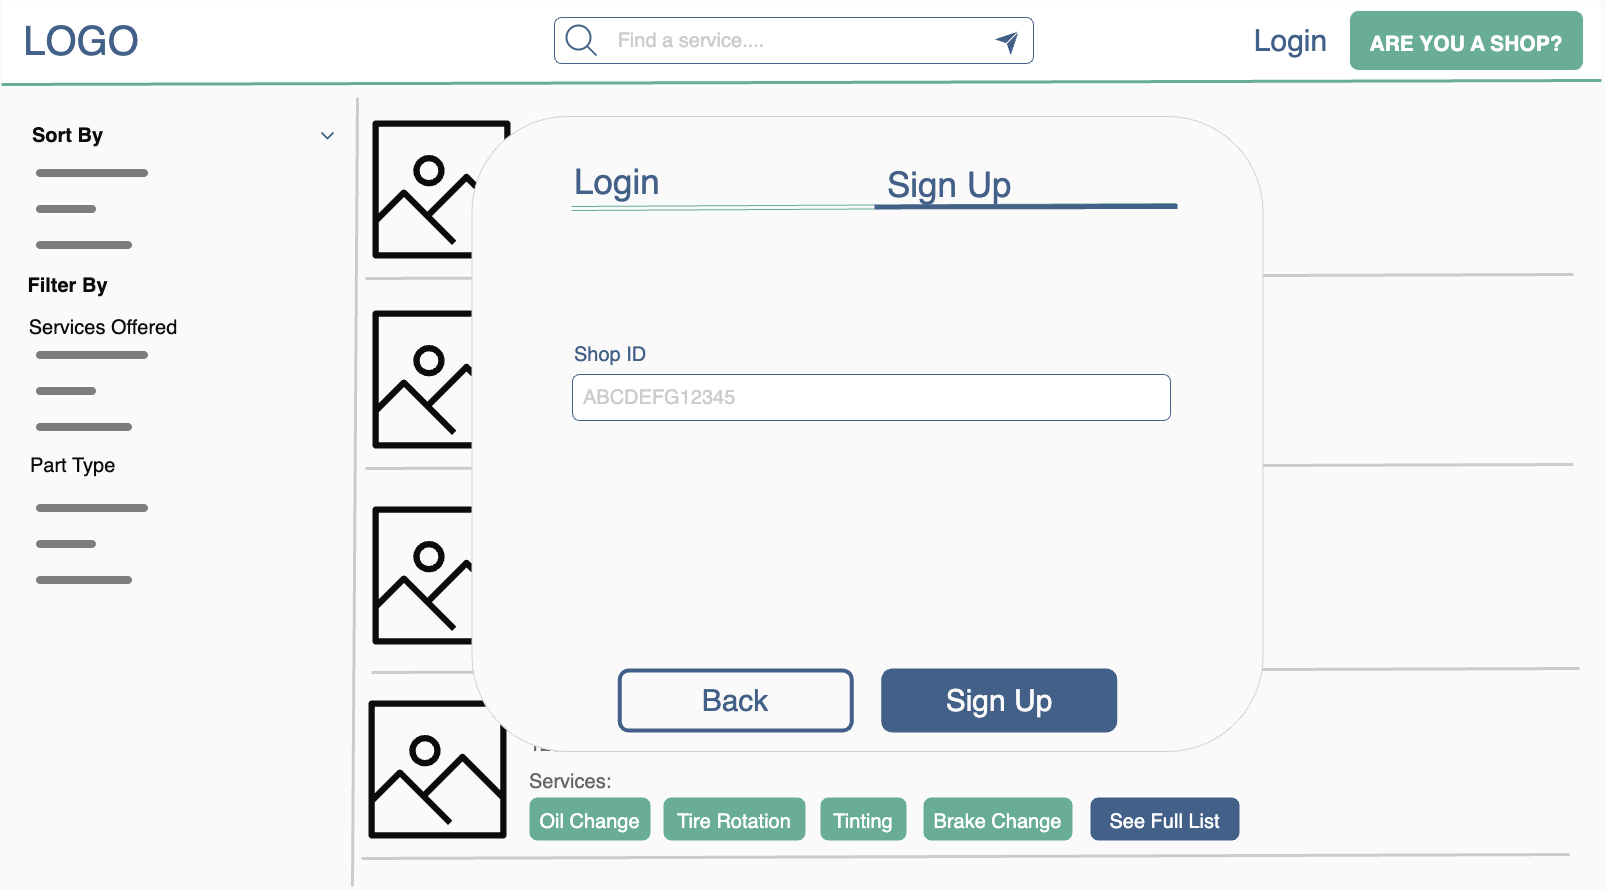
\includegraphics[width=\textwidth]{mockups/Employee Signup (Part 2) (Desktop).png}
	\caption{Employee Registration \textemdash{} Part 3 (Desktop)}
\end{figure}

\begin{figure}[H]
	\centering
	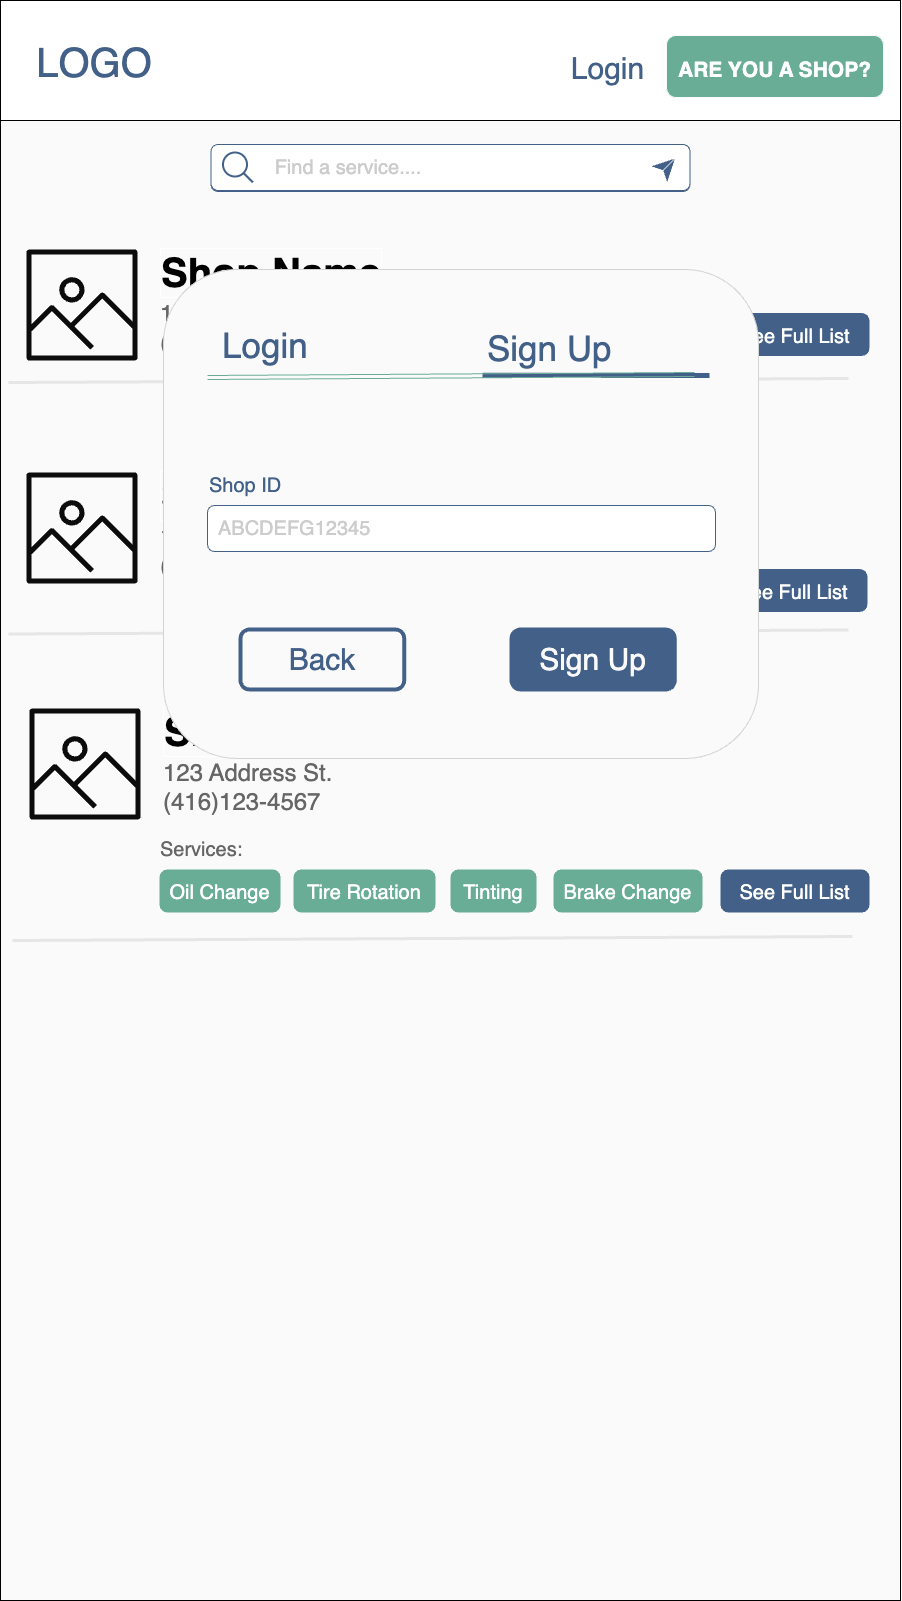
\includegraphics[width=0.5\textwidth]{mockups/Employee Signup (Part 2) (Mobile).png}
	\caption{Employee Registration \textemdash{} Part 3 (Mobile)}
\end{figure}

\subsection{Vehicle Owner Registration}

\begin{figure}[H]
	\centering
	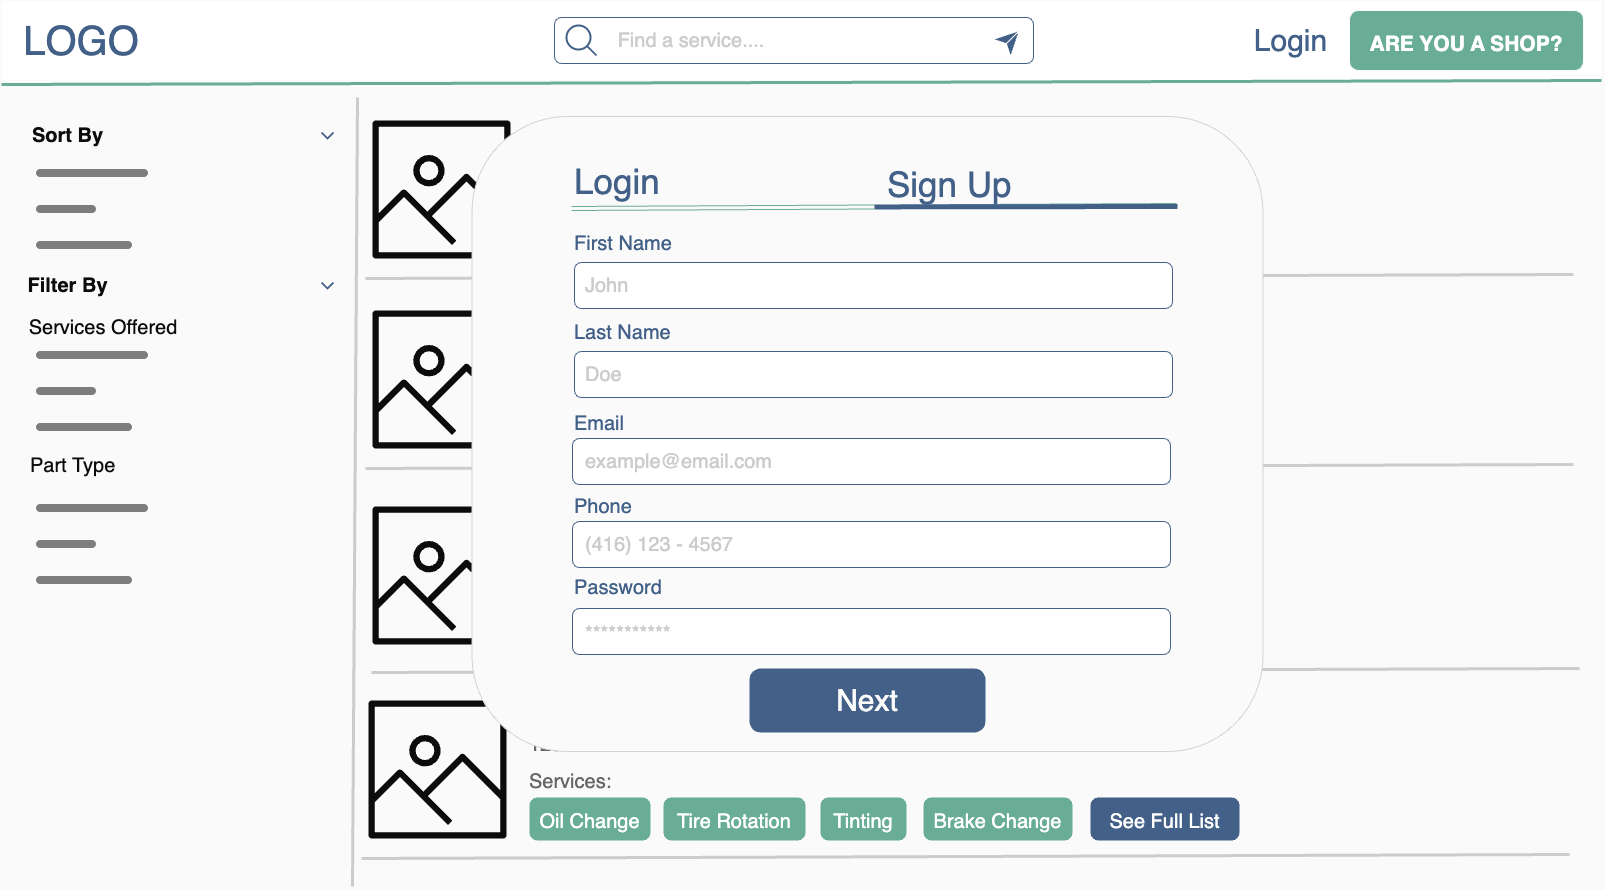
\includegraphics[width=\textwidth]{mockups/Vehicle Owner Sign Up (Part 1) (Desktop).png}
	\caption{Vehicle Owner Registration \textemdash{} Part 1 (Desktop)}
\end{figure}

\begin{figure}[H]
	\centering
	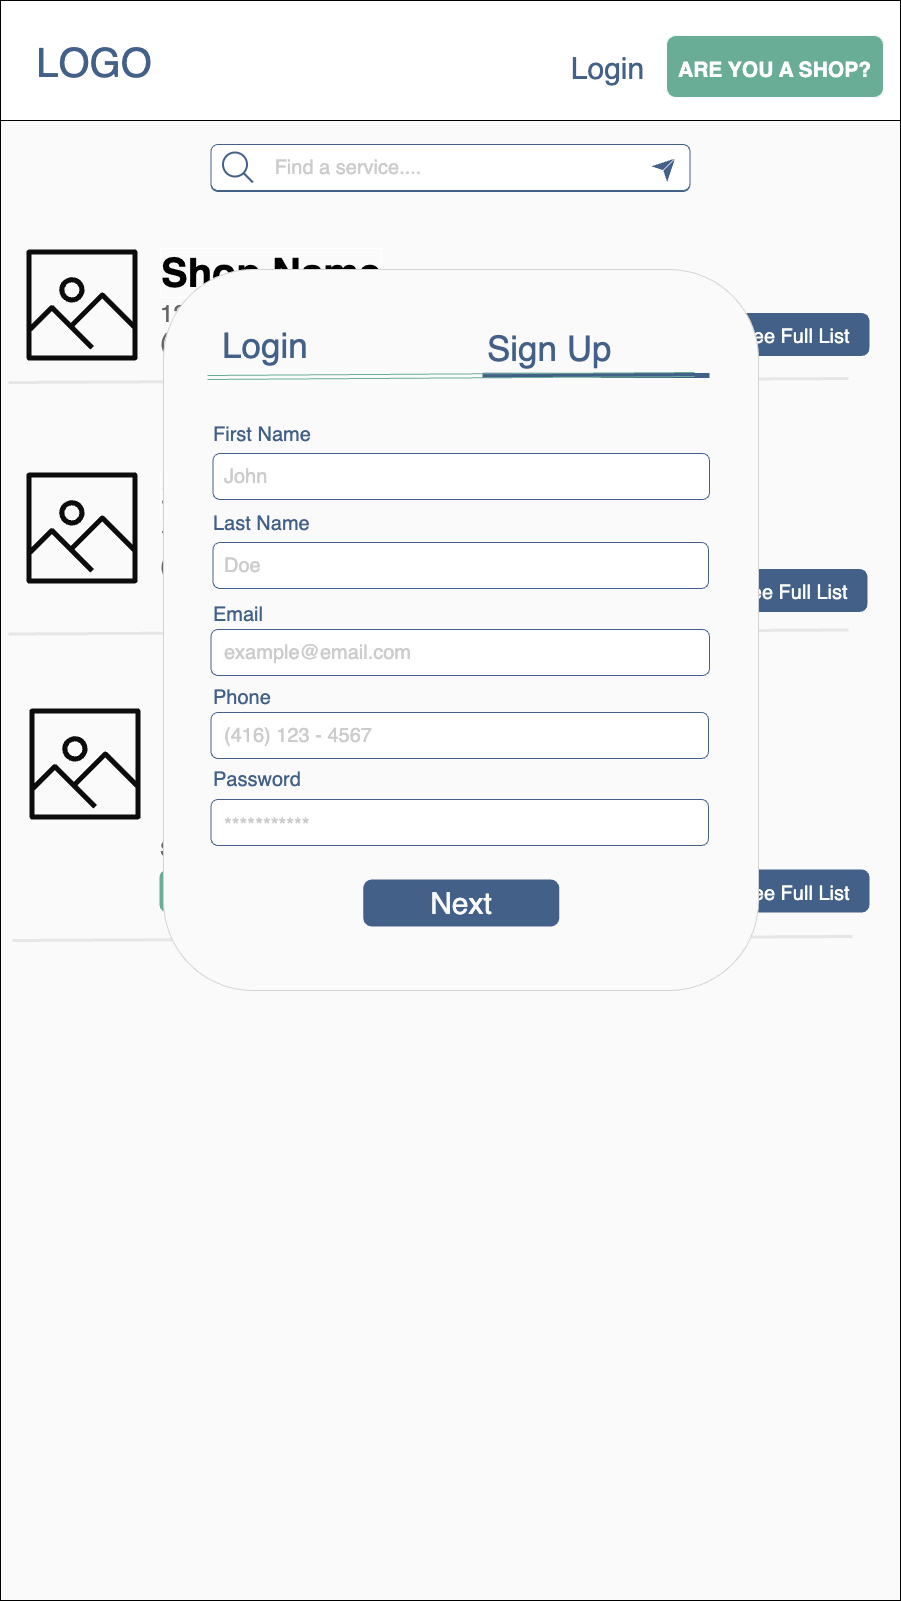
\includegraphics[width=0.5\textwidth]{mockups/Vehicle Owner Sign Up (Part 1) (Mobile).png}
	\caption{Vehicle Owner Registration \textemdash{} Part 1 (Mobile)}
\end{figure}

\begin{figure}[H]
	\centering
	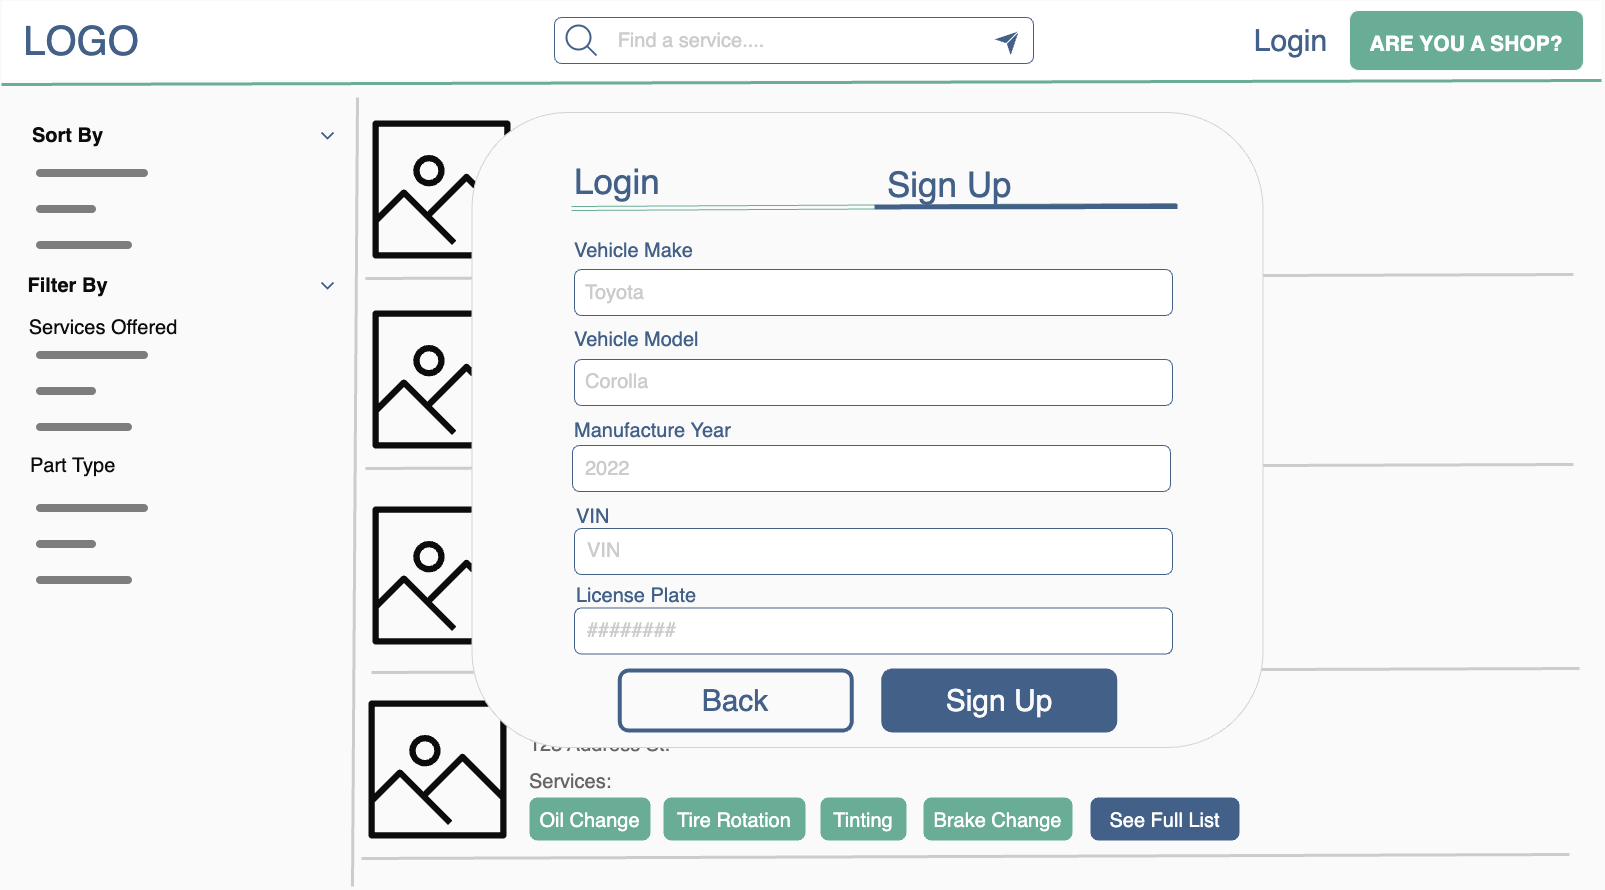
\includegraphics[width=\textwidth]{mockups/Vehicle Owner Sign Up (Part 2) (Desktop).png}
	\caption{Vehicle Owner Registration \textemdash{} Part 2 (Desktop)}
\end{figure}

\begin{figure}[H]
	\centering
	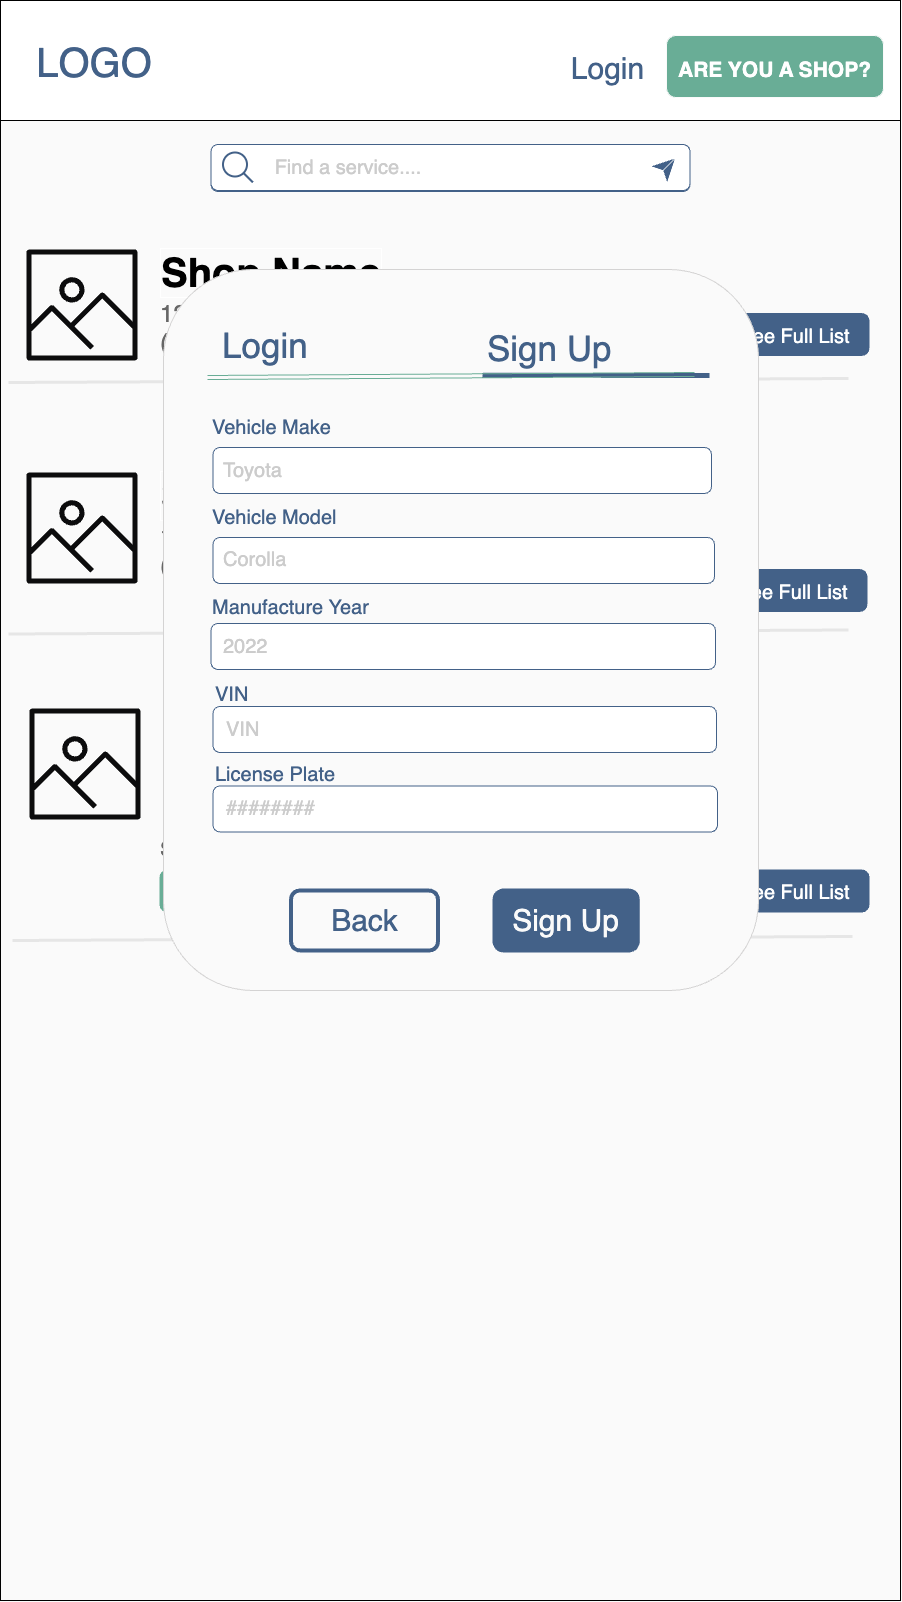
\includegraphics[width=0.5\textwidth]{mockups/Vehicle Owner Sign Up (Part 2) (Mobile).png}
	\caption{Vehicle Owner Registration \textemdash{} Part 2 (Mobile)}
\end{figure}

\subsection{Vehicle Owner/Shop Owner/Employee Login}

\begin{figure}[H]
	\centering
	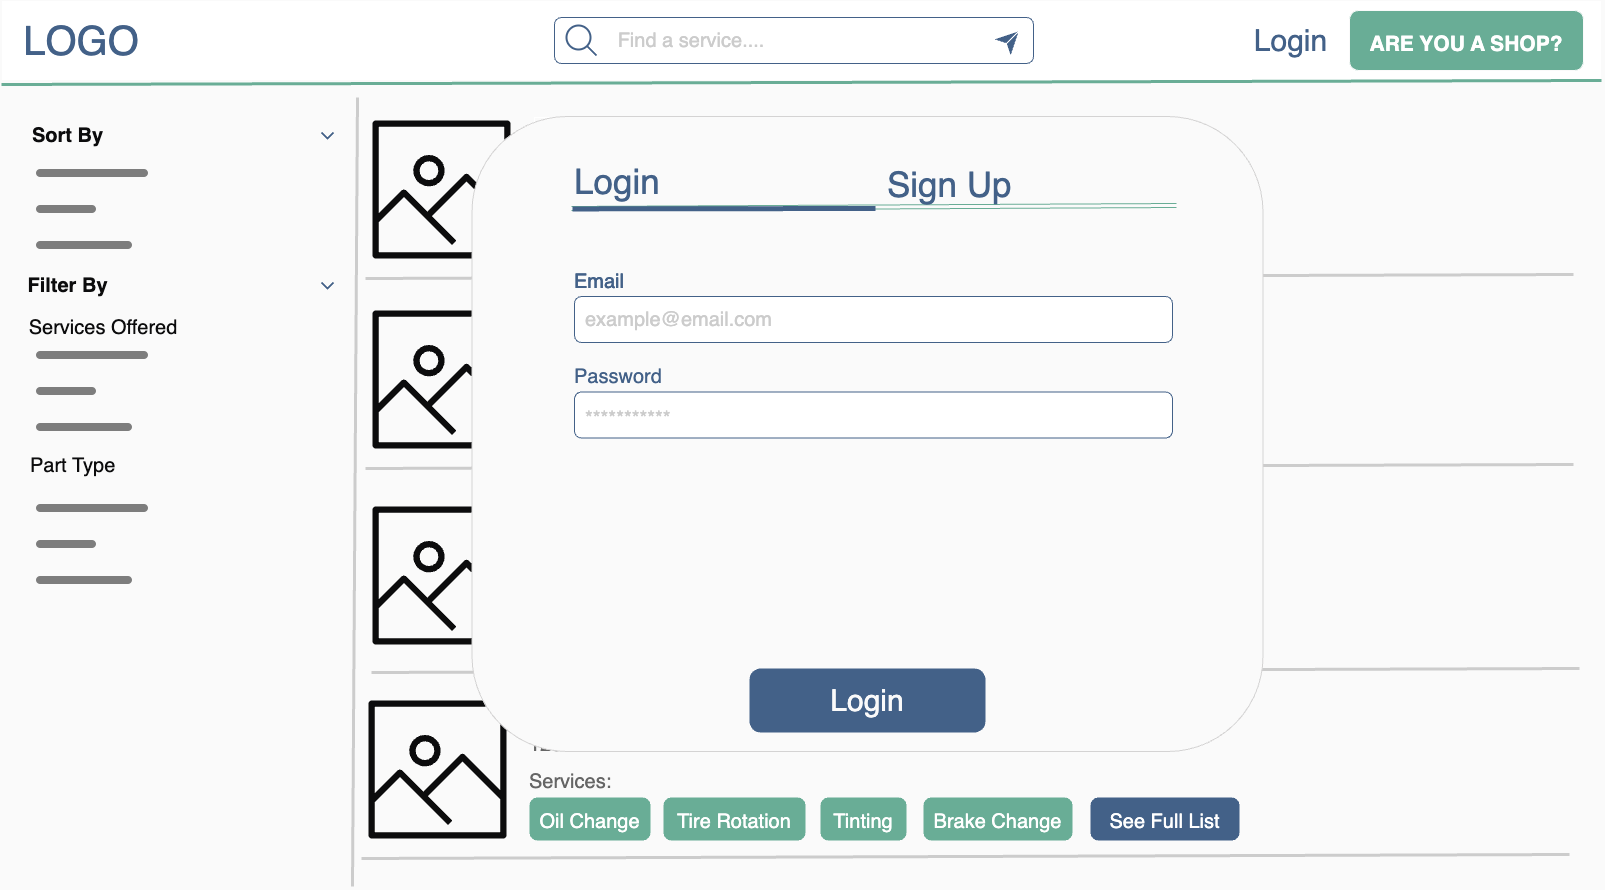
\includegraphics[width=\textwidth]{mockups/Vehicle-Shop Owner Login Popup (Desktop).png}
	\caption{Vehicle Owner/Shop Owner/Employee Login (Desktop)}
\end{figure}

\begin{figure}[H]
	\centering
	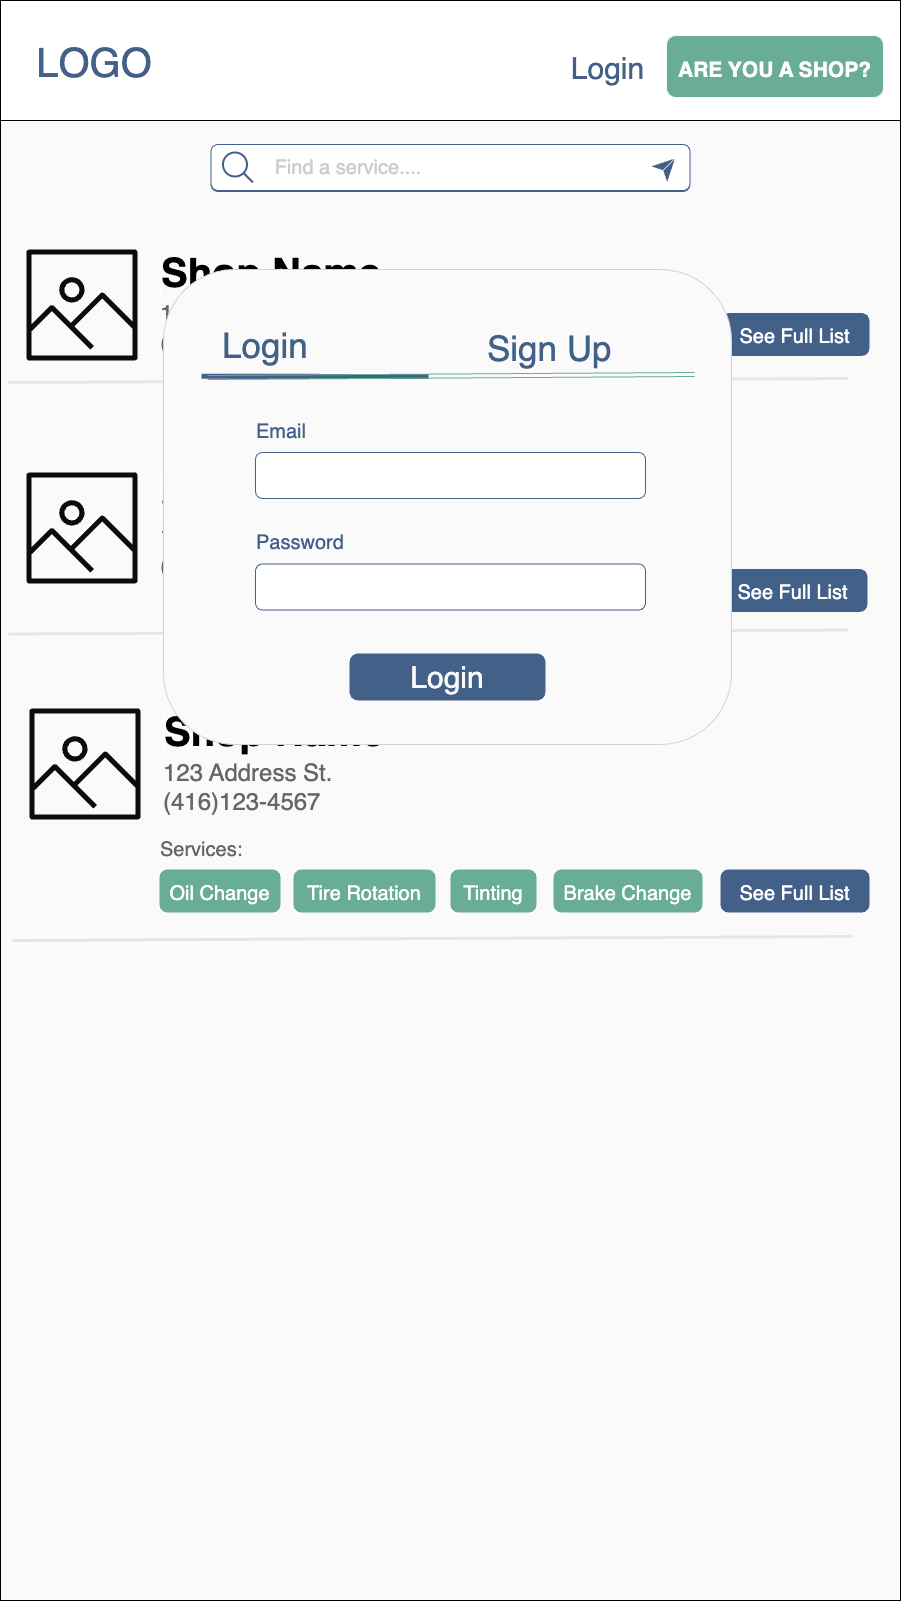
\includegraphics[width=0.5\textwidth]{mockups/Vehicle-Shop Owner Login Popup (Mobile).png}
	\caption{Vehicle Owner/Shop Owner/Employee Login (Mobile)}
\end{figure}

\subsection{Vehicle Owner Dashboard}
\subsubsection{Service Requests}

\begin{figure}[H]
	\centering
	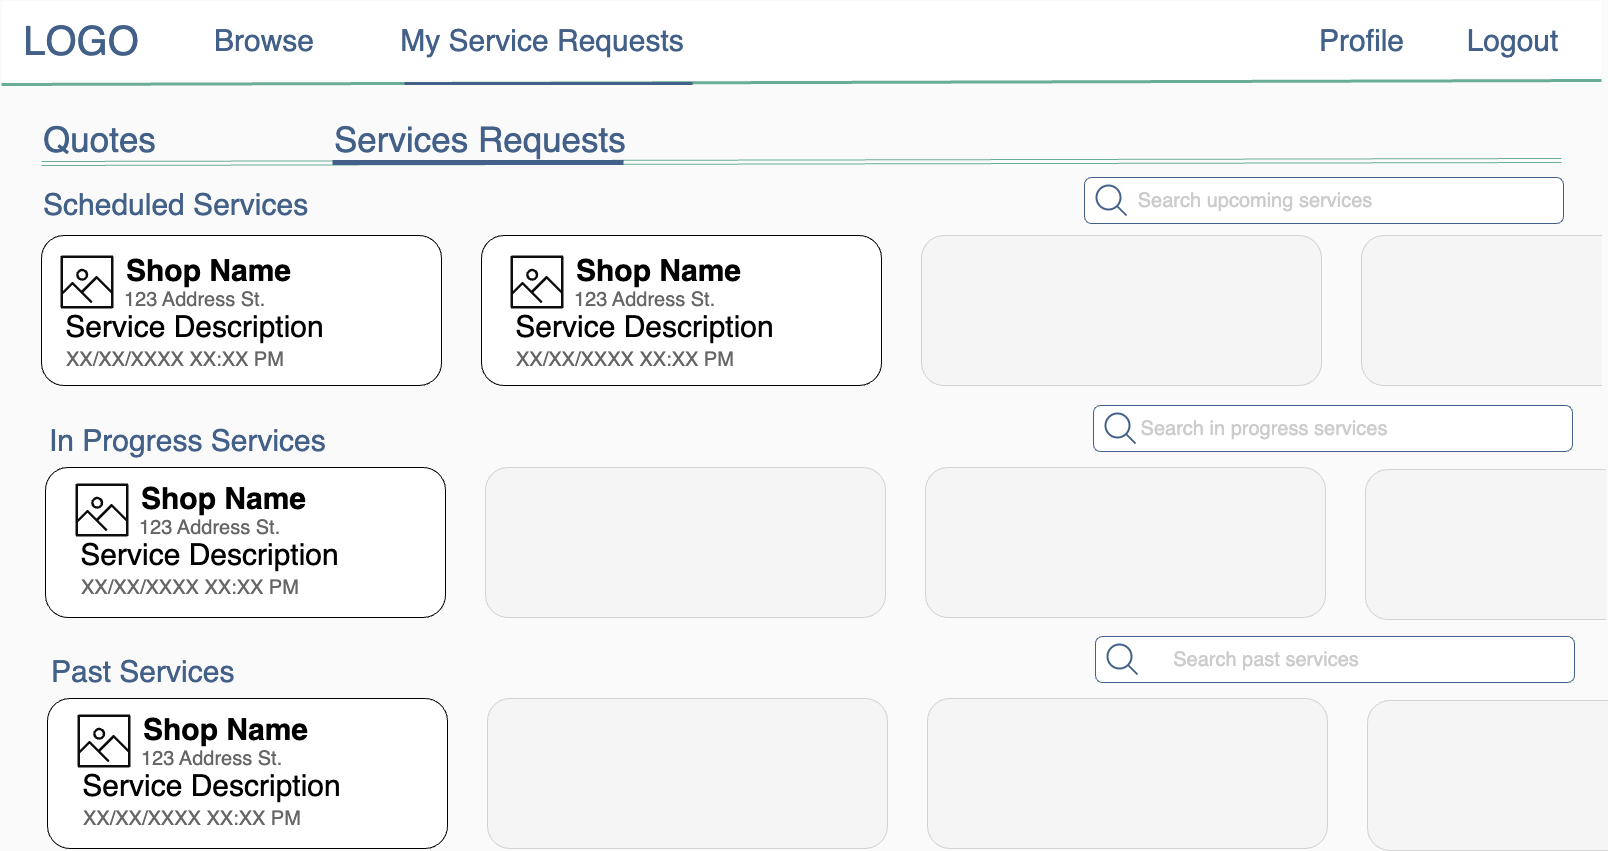
\includegraphics[width=\textwidth]{mockups/Vehicle Owner Dashboard (Service Requests) (Desktop).png}
	\caption{Vehicle Owner Dashboard \textemdash{} Service Requests (Desktop)}
\end{figure}

\begin{figure}[H]
	\centering
	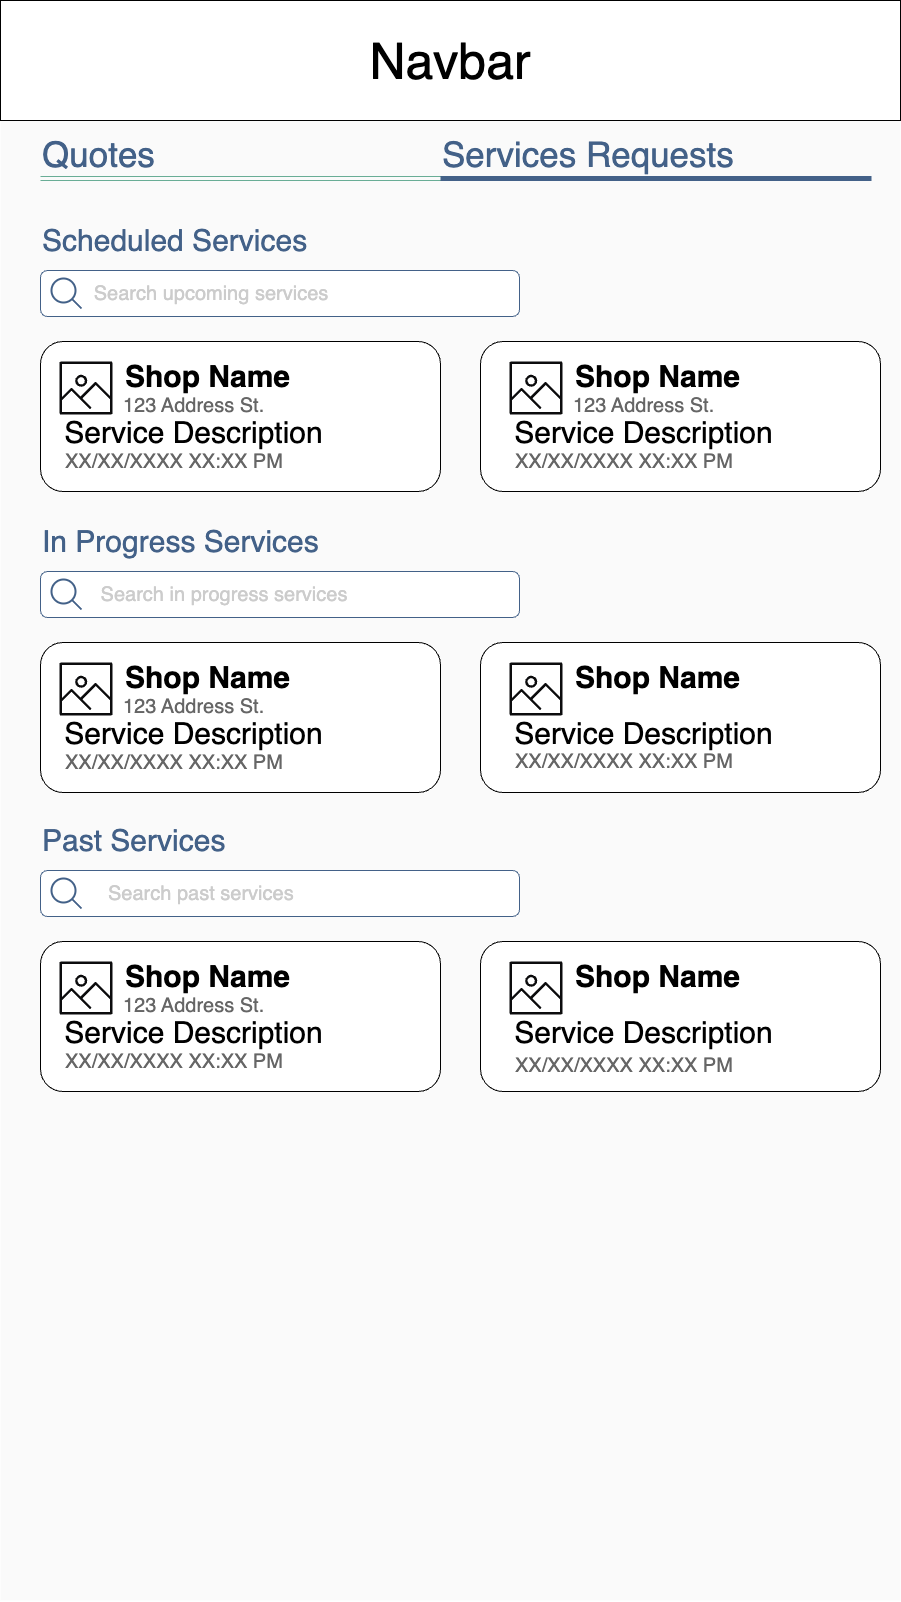
\includegraphics[width=0.5\textwidth]{mockups/Vehicle Owner Dashboard (Service Requests) (Mobile).png}
	\caption{Vehicle Owner Dashboard \textemdash{} Service Requests (Mobile)}
\end{figure}

\subsubsection{Quotes}

\begin{figure}[H]
	\centering
	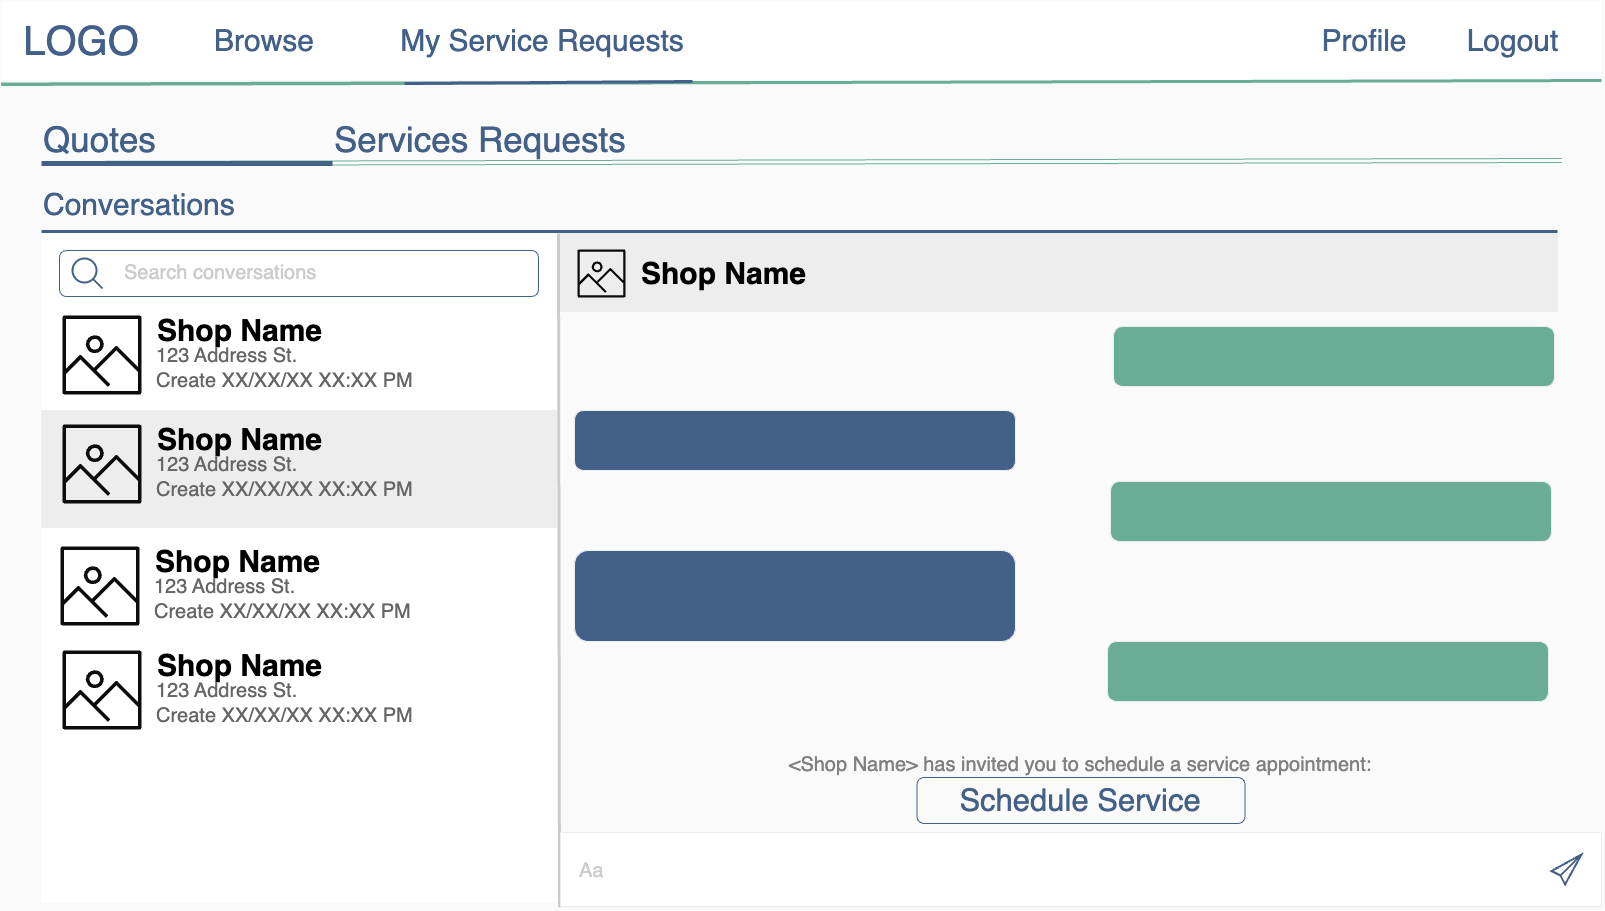
\includegraphics[width=\textwidth]{mockups/Vehicle Owner Dashboard (Quotes) (Desktop).png}
	\caption{Vehicle Owner Dashboard \textemdash{} Quotes (Desktop)}
\end{figure}

\begin{figure}[H]
	\centering
	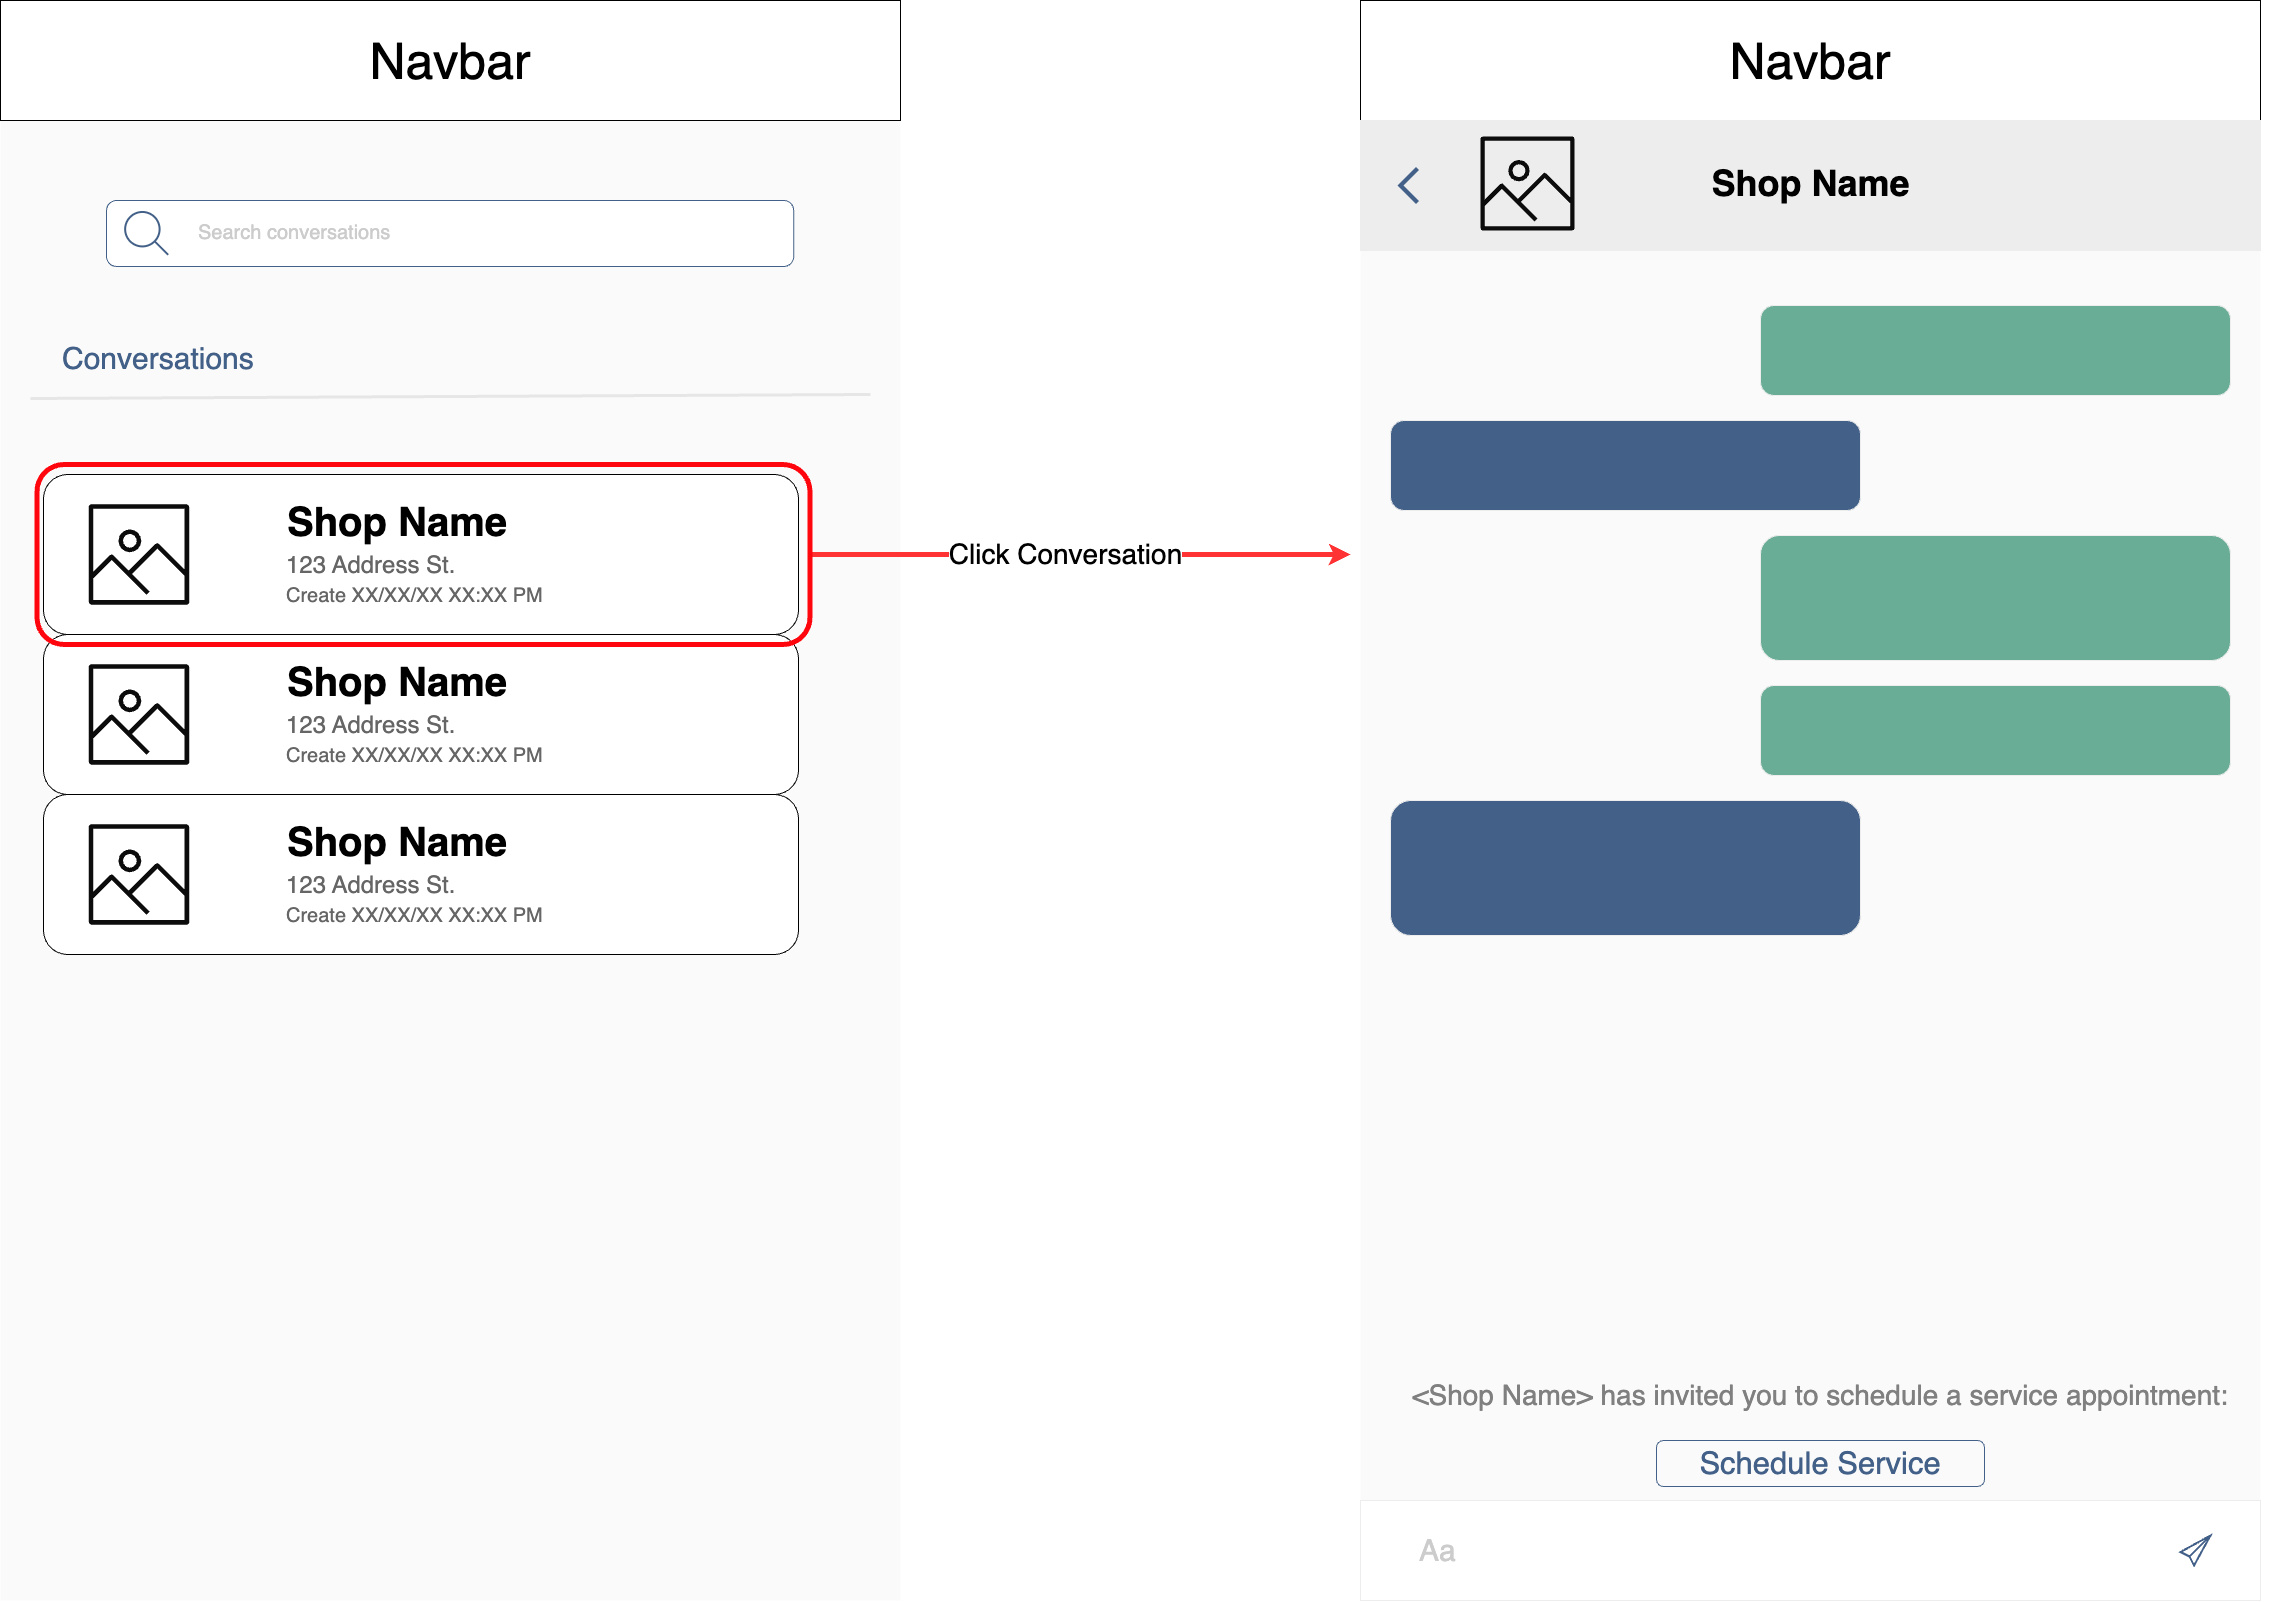
\includegraphics[width=\textwidth]{mockups/Vehicle Owner Dashboard (Quotes) (Mobile).png}
	\caption{Vehicle Owner Dashboard \textemdash{} Quotes (Mobile)}
\end{figure}

\subsection{Vehicle Owner Create Appointment}

\begin{figure}[H]
	\centering
	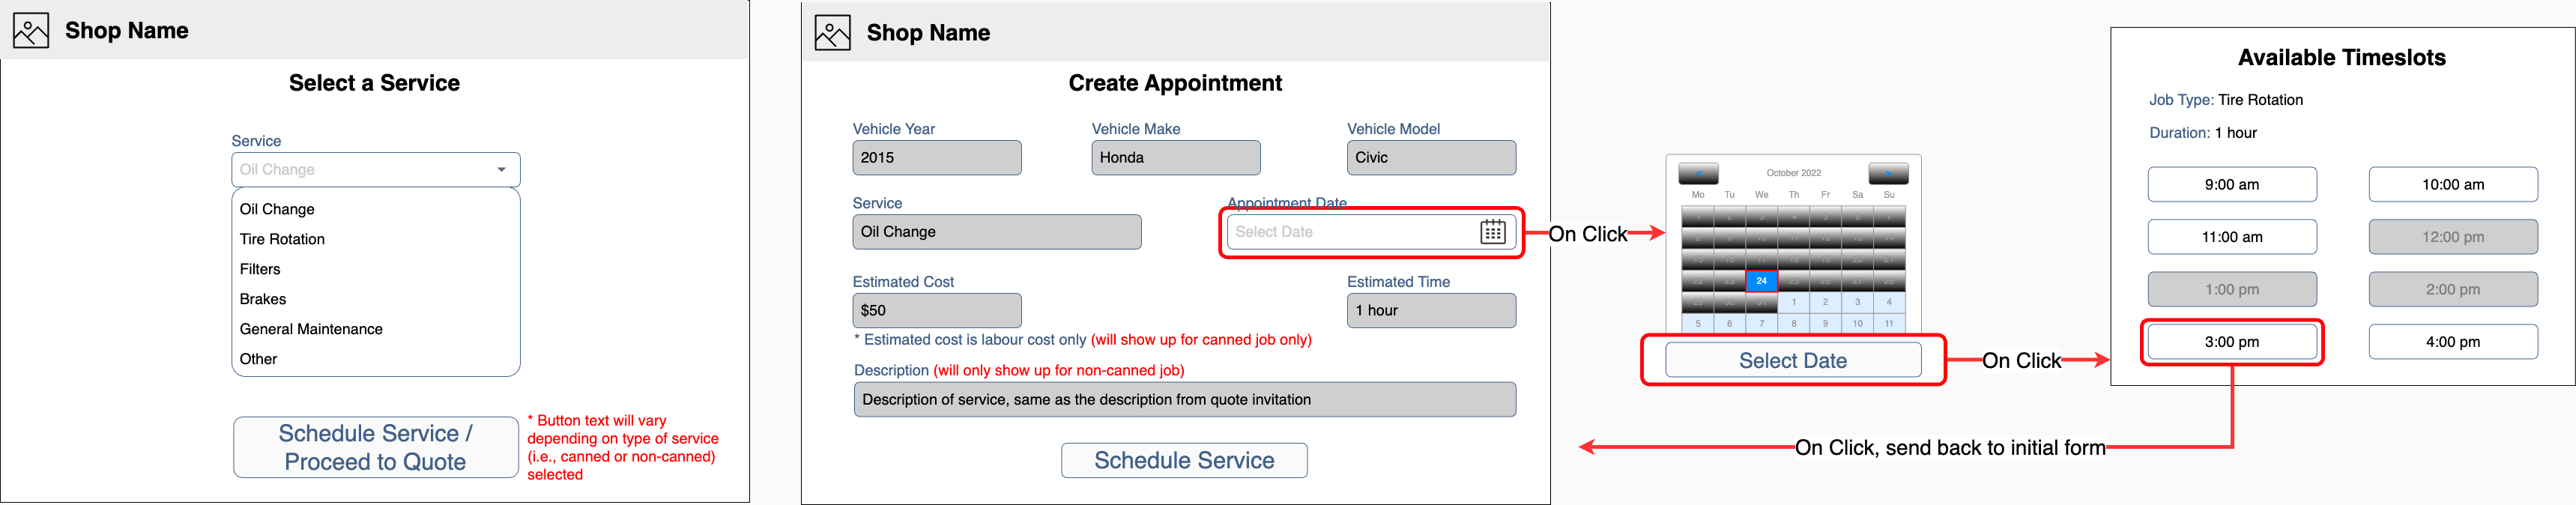
\includegraphics[width=\textwidth]{mockups/Vehicle Owner - Create Appointment Popup (Desktop).png}
	\caption{Vehicle Owner Create Appointment (Desktop)}
\end{figure}

\subsection{Shop Owner/Employee Dashboard}
\subsubsection{Quotes Requests}

\begin{figure}[H]
	\centering
	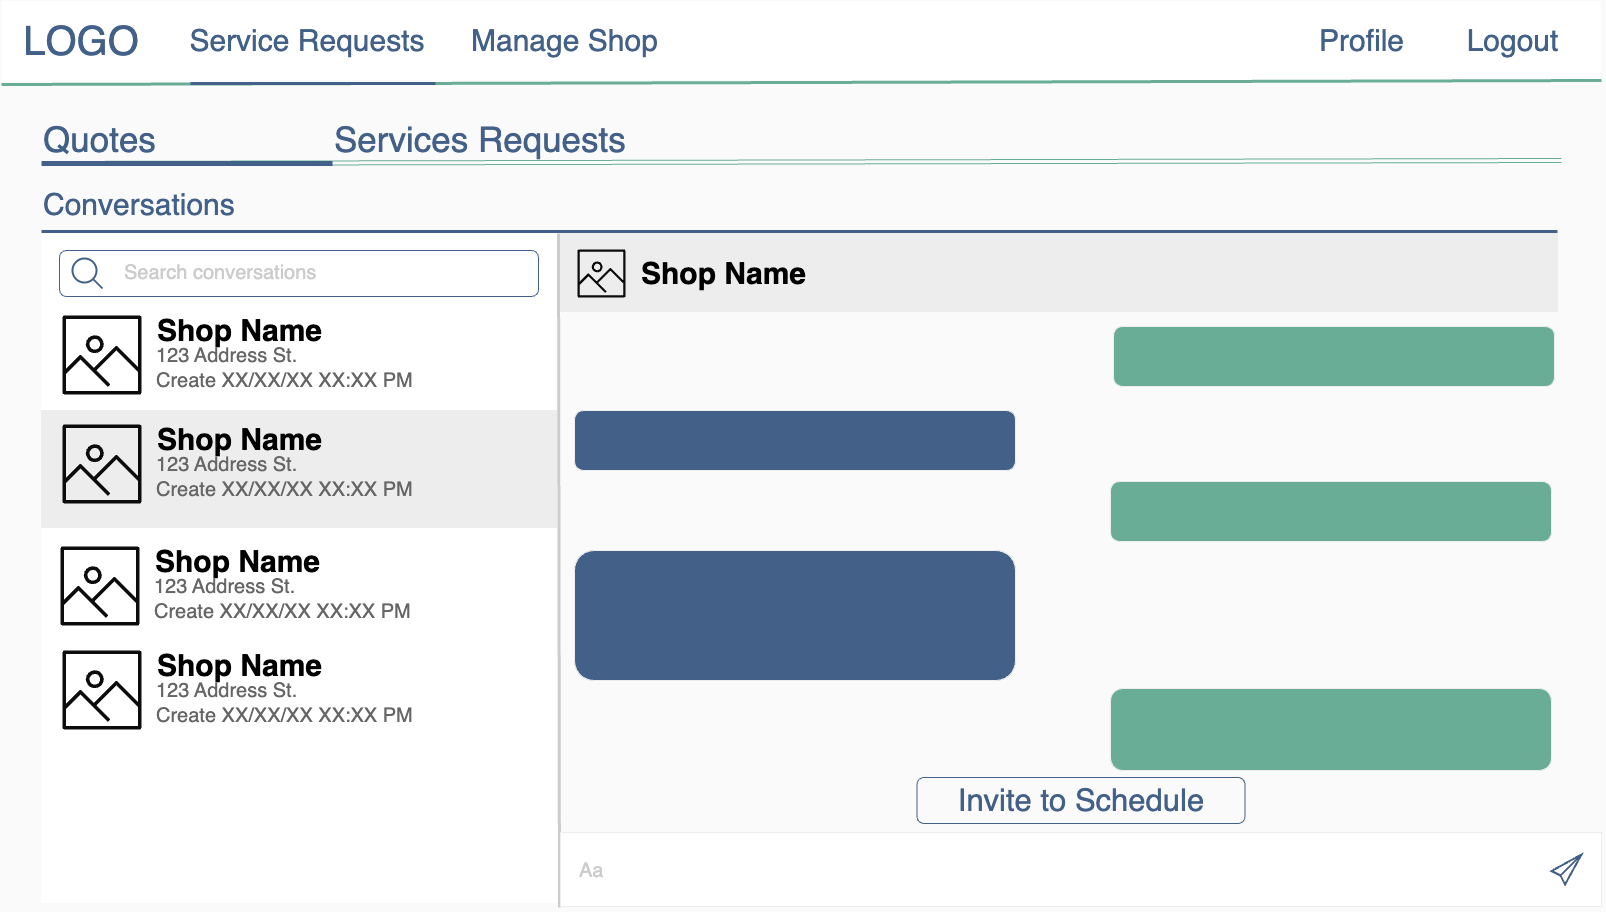
\includegraphics[width=\textwidth]{mockups/Shop Owner Dashboard (Quotes Requests) (Desktop).png}
	\caption{Shop Owner/Employee Dashboard \textemdash{} Quotes Requests (Desktop)}
\end{figure}

\begin{figure}[H]
	\centering
	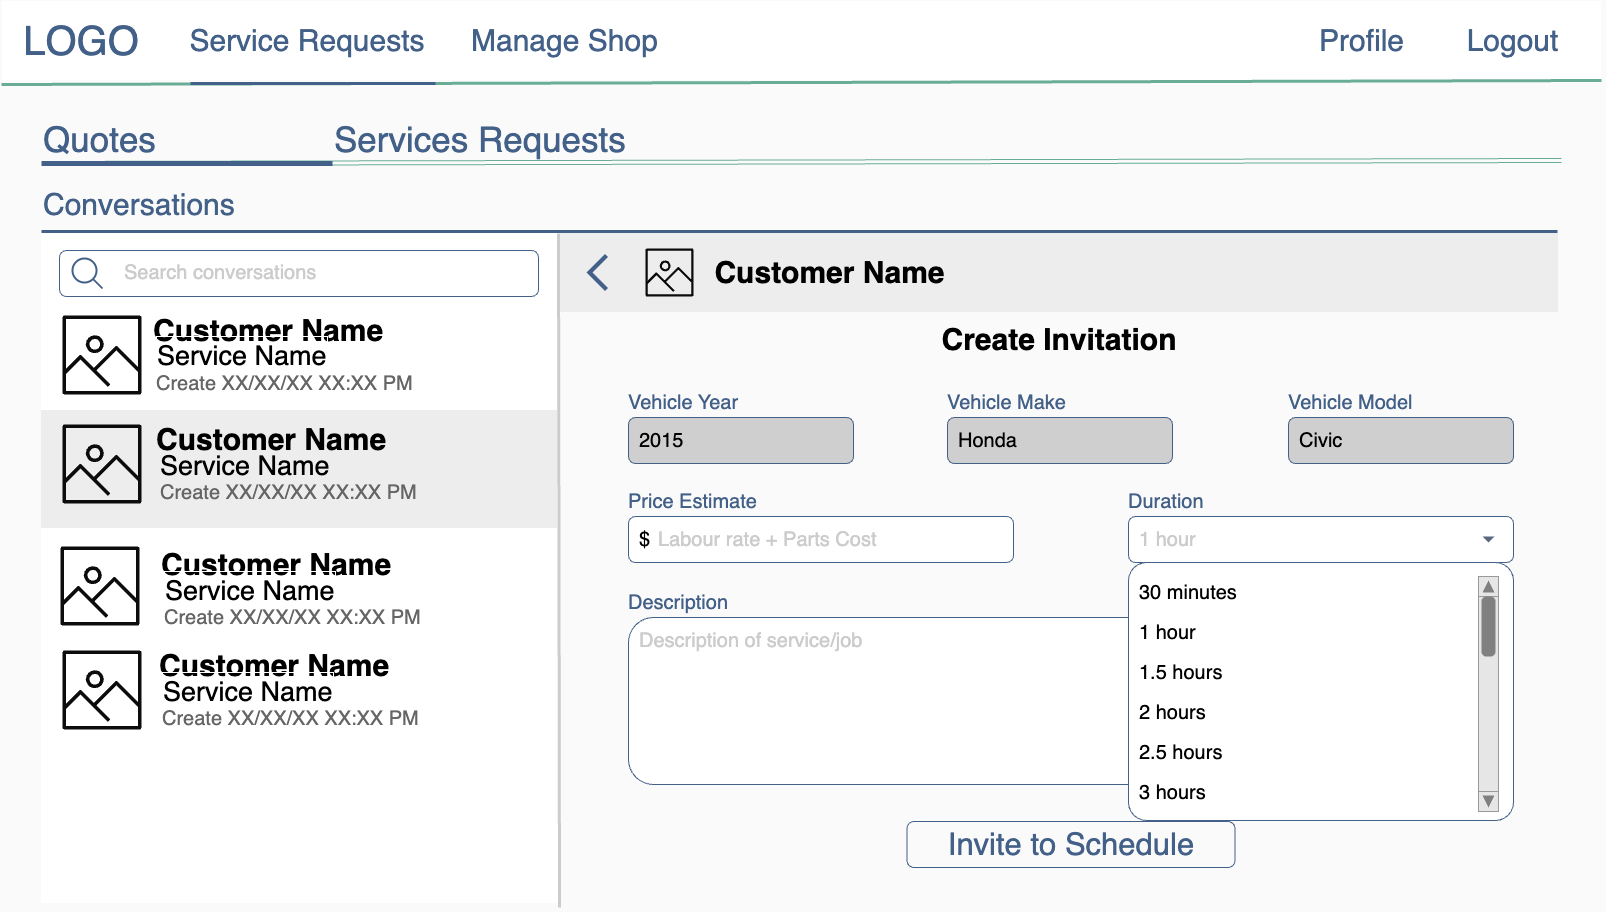
\includegraphics[width=\textwidth]{mockups/Shop Owner Dashboard (Quotes Requests - Invitation) (Desktop).png}
	\caption{Shop Owner/Employee Dashboard \textemdash{} Quotes Requests \textemdash{} Invitation (Desktop)}
\end{figure}

\subsubsection{Service Requests \textemdash{} Requested}

\begin{figure}[H]
	\centering
	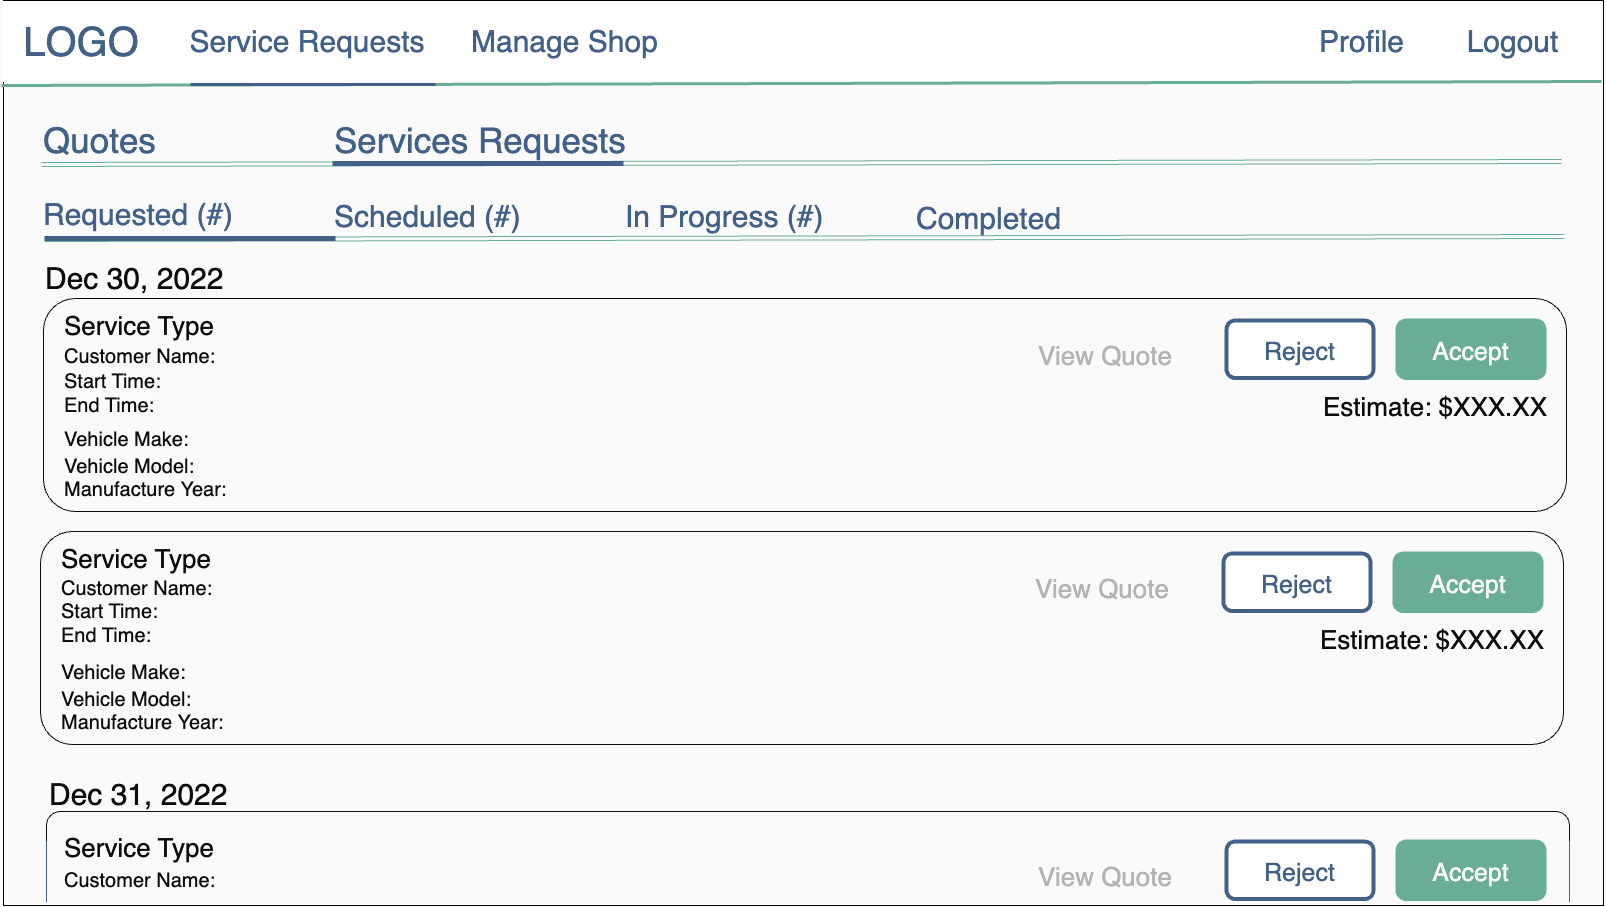
\includegraphics[width=\textwidth]{mockups/Shop Owner Dashboard (Service Requests - Requested) (Desktop).png}
	\caption{Shop Owner/Employee Dashboard \textemdash{} Service \textemdash{} Requested (Desktop)}
\end{figure}

\begin{figure}[H]
	\centering
	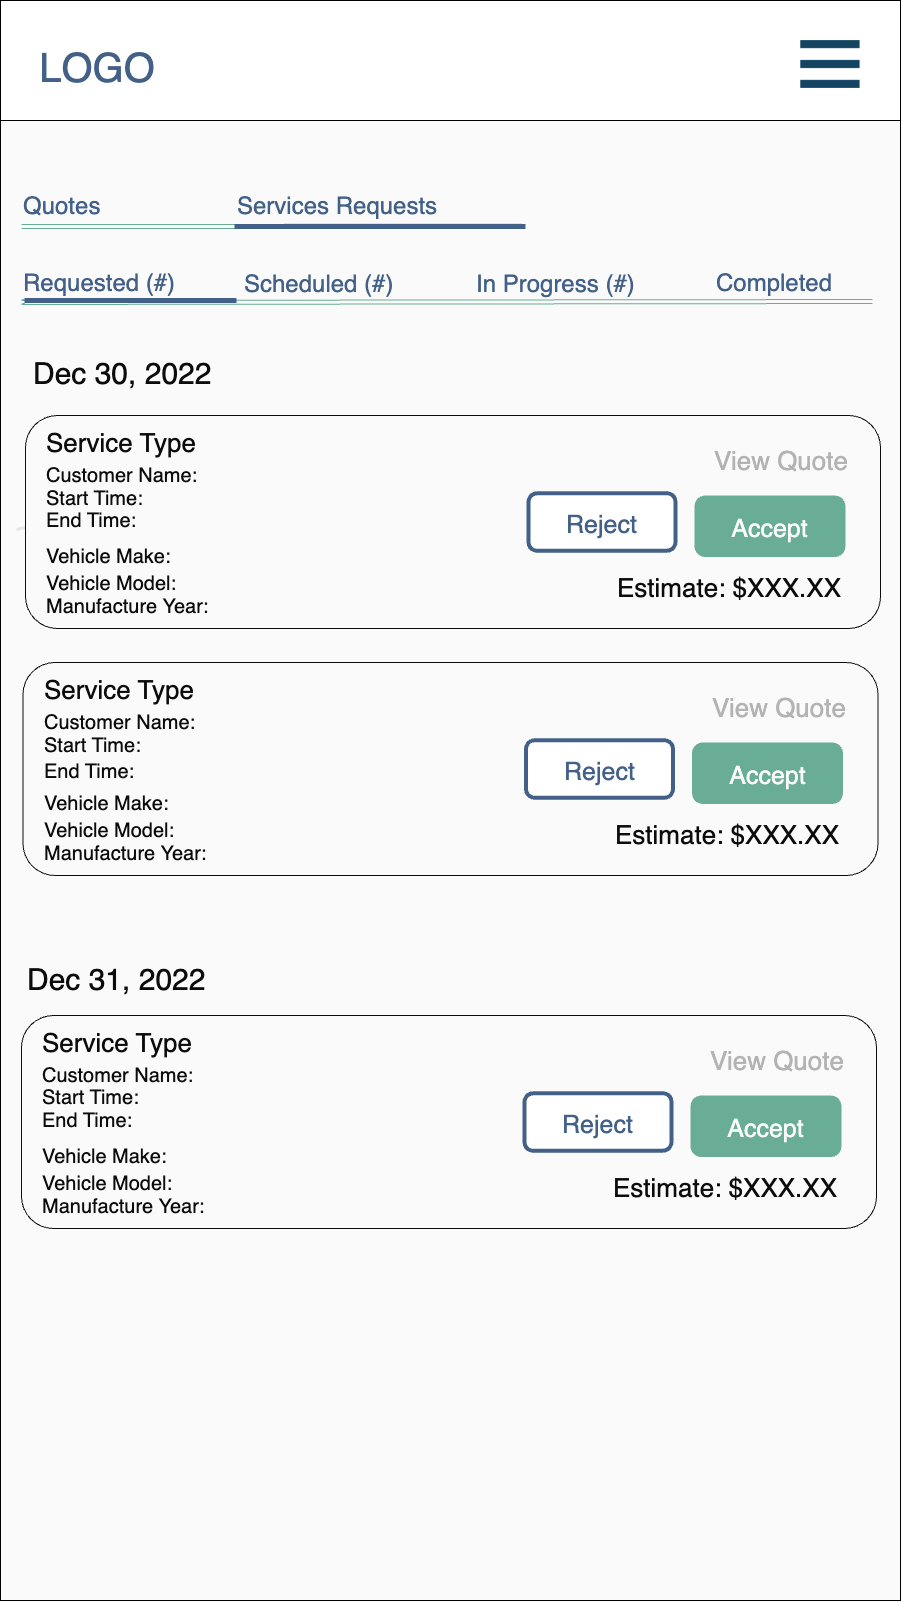
\includegraphics[width=0.5\textwidth]{mockups/Shop Owner Dashboard (Service Requests - Requested) (Mobile).png}
	\caption{Shop Owner/Employee Dashboard \textemdash{} Service \textemdash{} Requested (Mobile)}
\end{figure}

\subsubsection{Service Requests \textemdash{} Scheduled}

\begin{figure}[H]
	\centering
	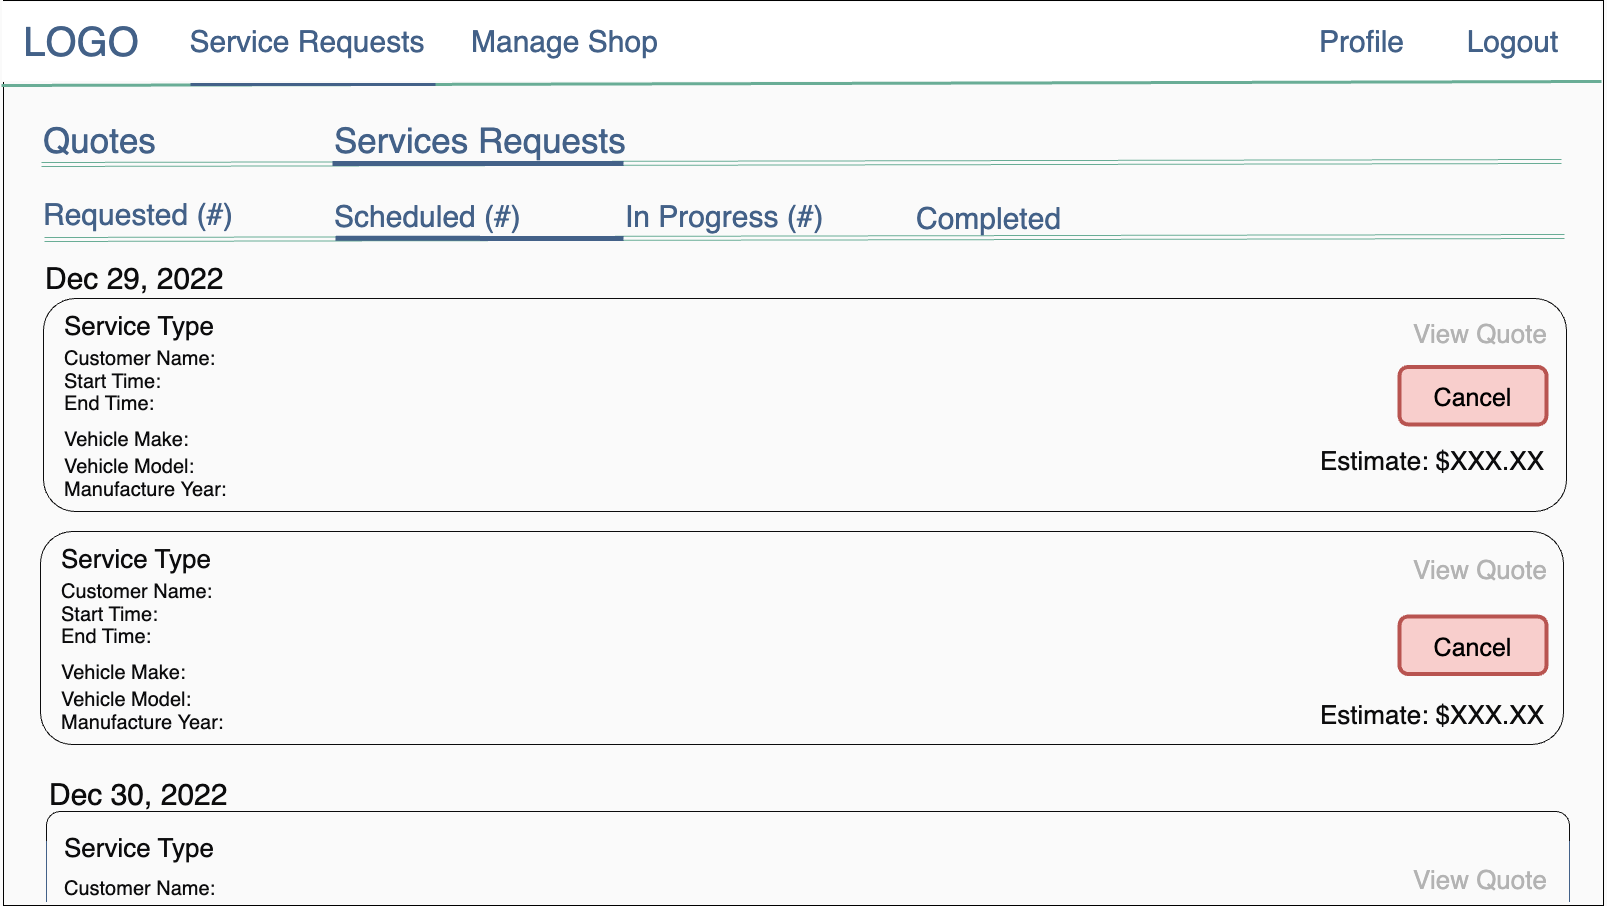
\includegraphics[width=\textwidth]{mockups/Shop Owner Dashboard (Service Requests - Scheduled) (Desktop).png}
	\caption{Shop Owner/Employee Dashboard \textemdash{} Service \textemdash{} Scheduled (Desktop)}
\end{figure}

\begin{figure}[H]
	\centering
	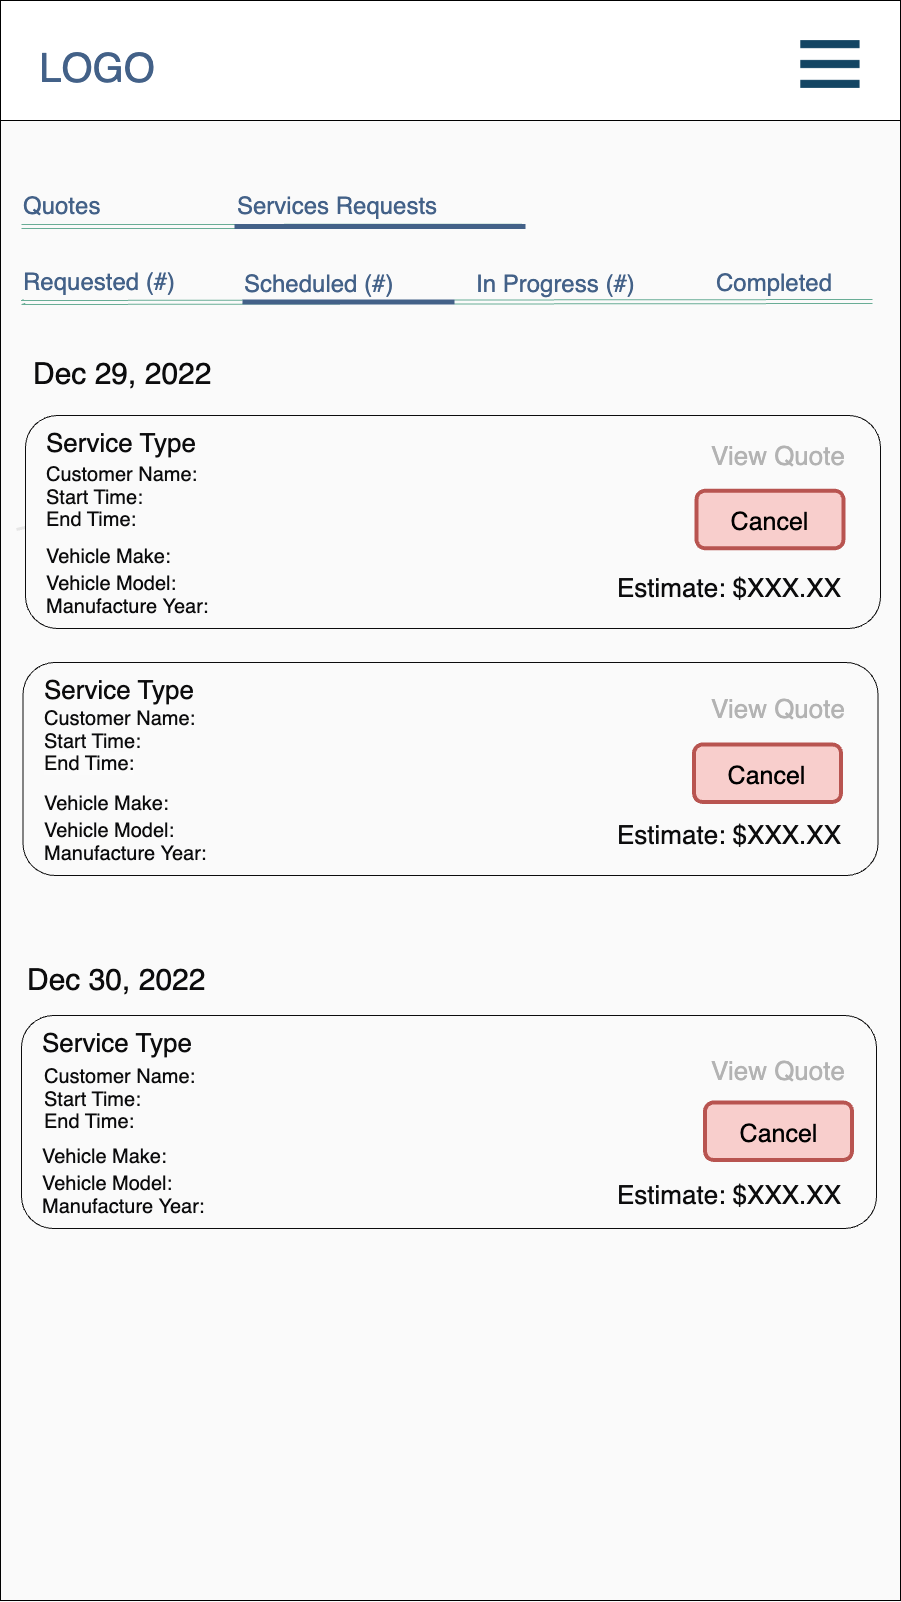
\includegraphics[width=0.5\textwidth]{mockups/Shop Owner Dashboard (Service Requests - Scheduled) (Mobile).png}
	\caption{Shop Owner/Employee Dashboard \textemdash{} Service \textemdash{} Scheduled (Mobile)}
\end{figure}

\subsubsection{Service Requests \textemdash{} In Progress}

\begin{figure}[H]
	\centering
	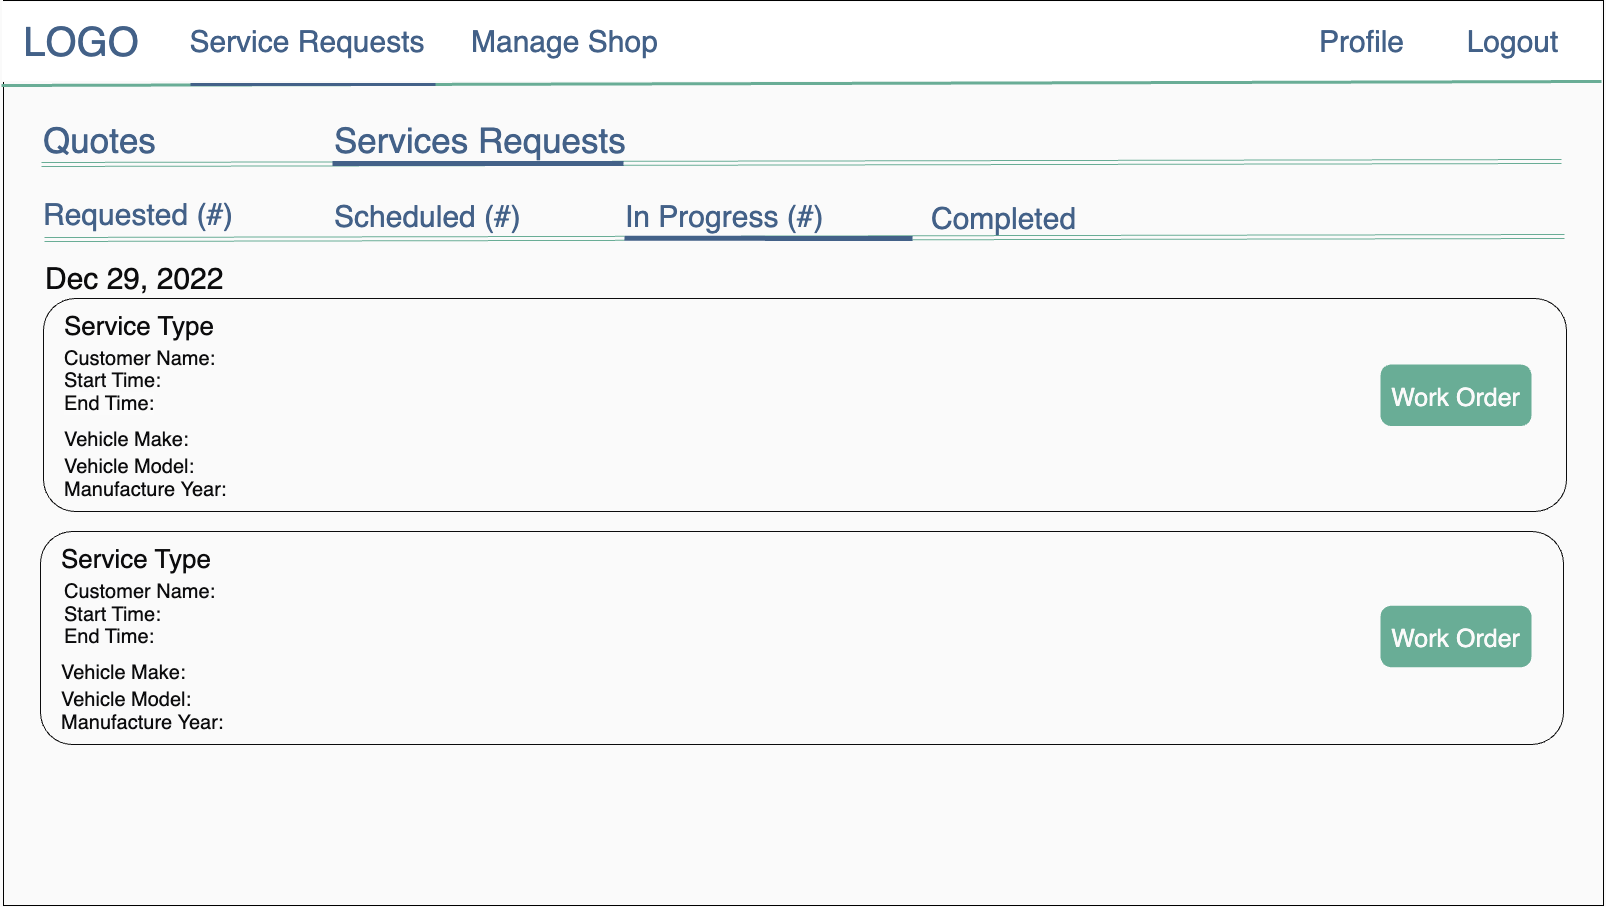
\includegraphics[width=\textwidth]{mockups/Shop Owner Dashboard (Service Requests - In Progress) (Desktop).png}
	\caption{Shop Owner/Employee Dashboard \textemdash{} Service \textemdash{} In Progress (Desktop)}
\end{figure}

\begin{figure}[H]
	\centering
	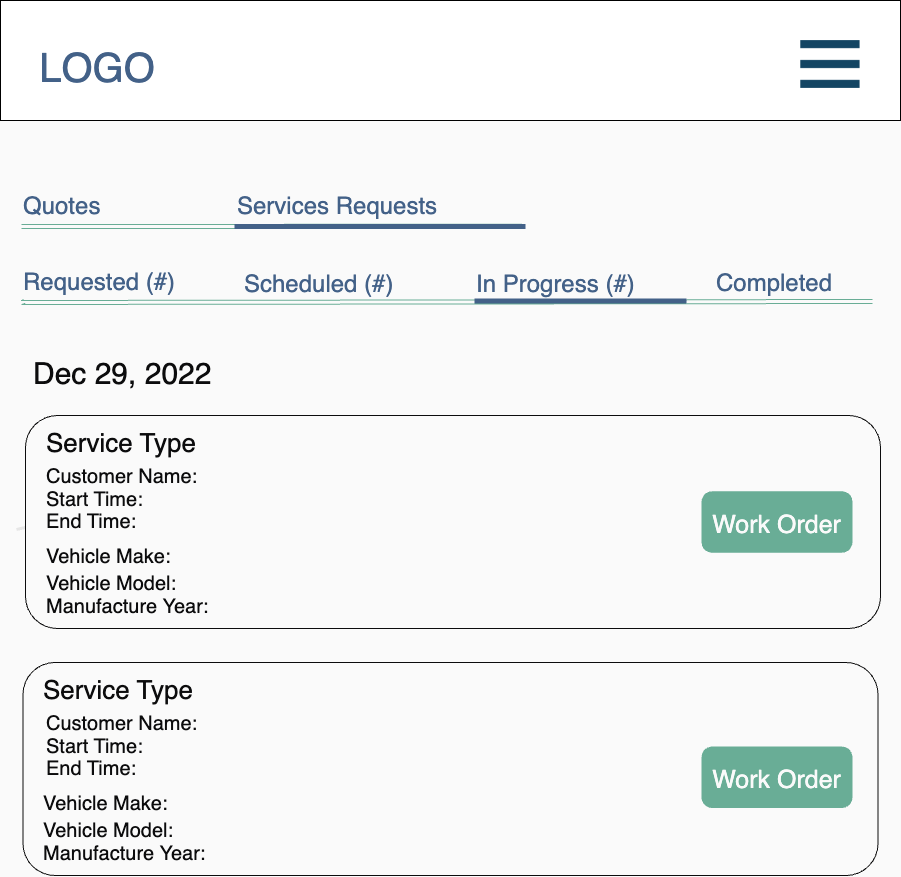
\includegraphics[width=0.5\textwidth]{mockups/Shop Owner Dashboard (Service Requests - In Progress) (Mobile).png}
	\caption{Shop Owner/Employee Dashboard \textemdash{} Service \textemdash{} In Progress (Mobile)}
\end{figure}

\subsubsection{Service Requests \textemdash{} Work Orders}

\begin{figure}[H]
	\centering
	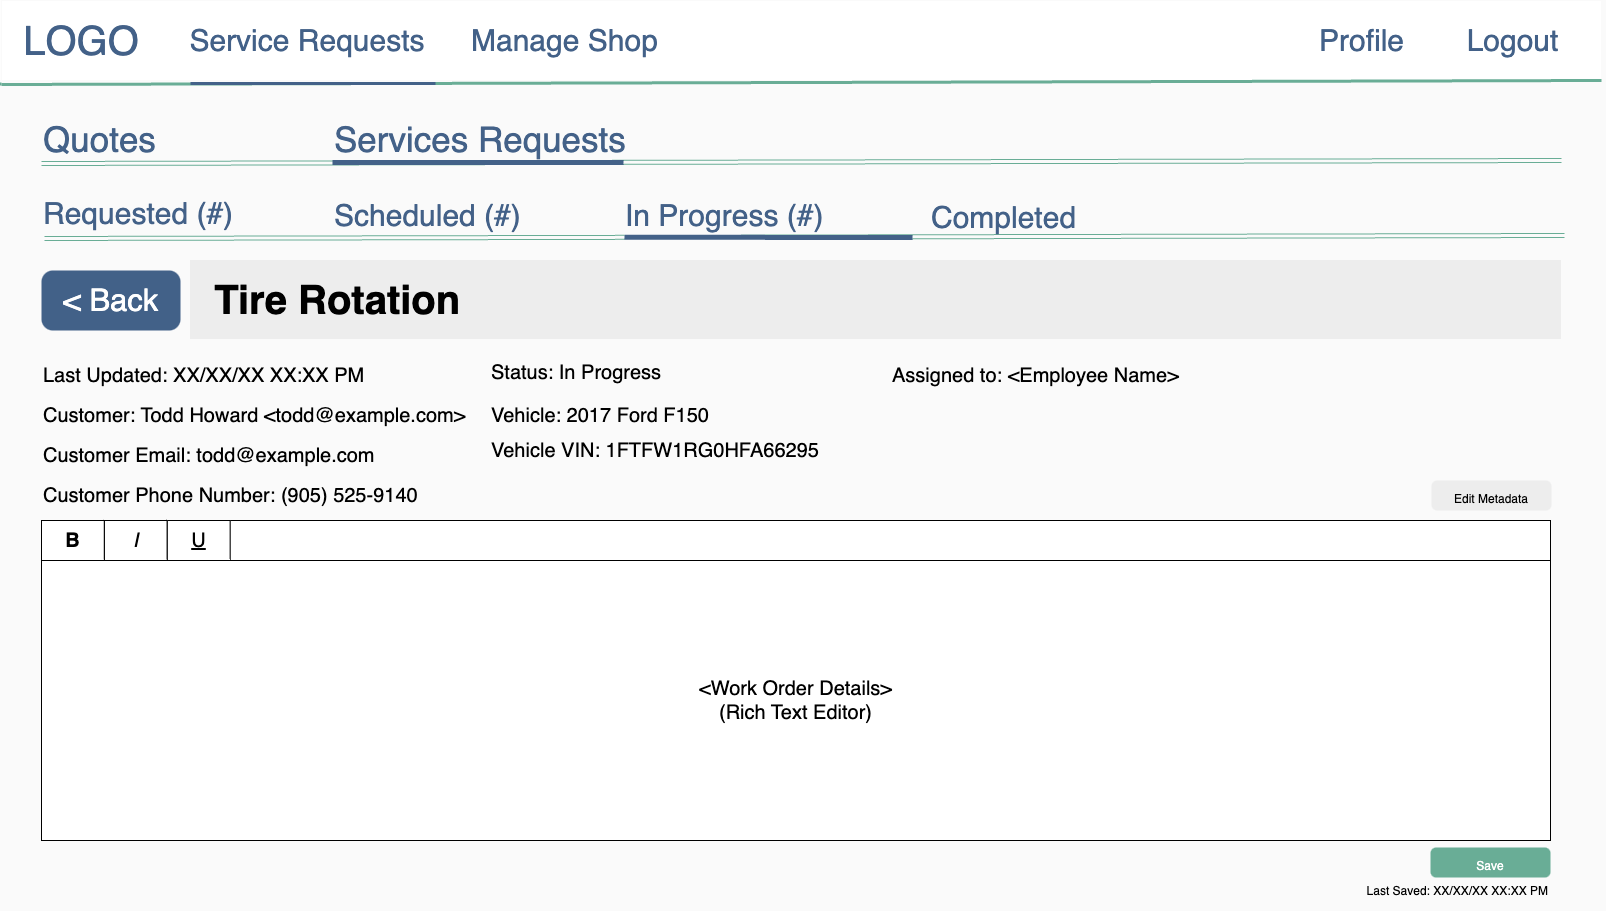
\includegraphics[width=\textwidth]{mockups/Shop Owner-Employee Work Order (Desktop).png}
	\caption{Shop Owner/Employee Dashboard \textemdash{} Service Requests \textemdash{} Work Orders (Desktop)}
\end{figure}

\begin{figure}[H]
	\centering
	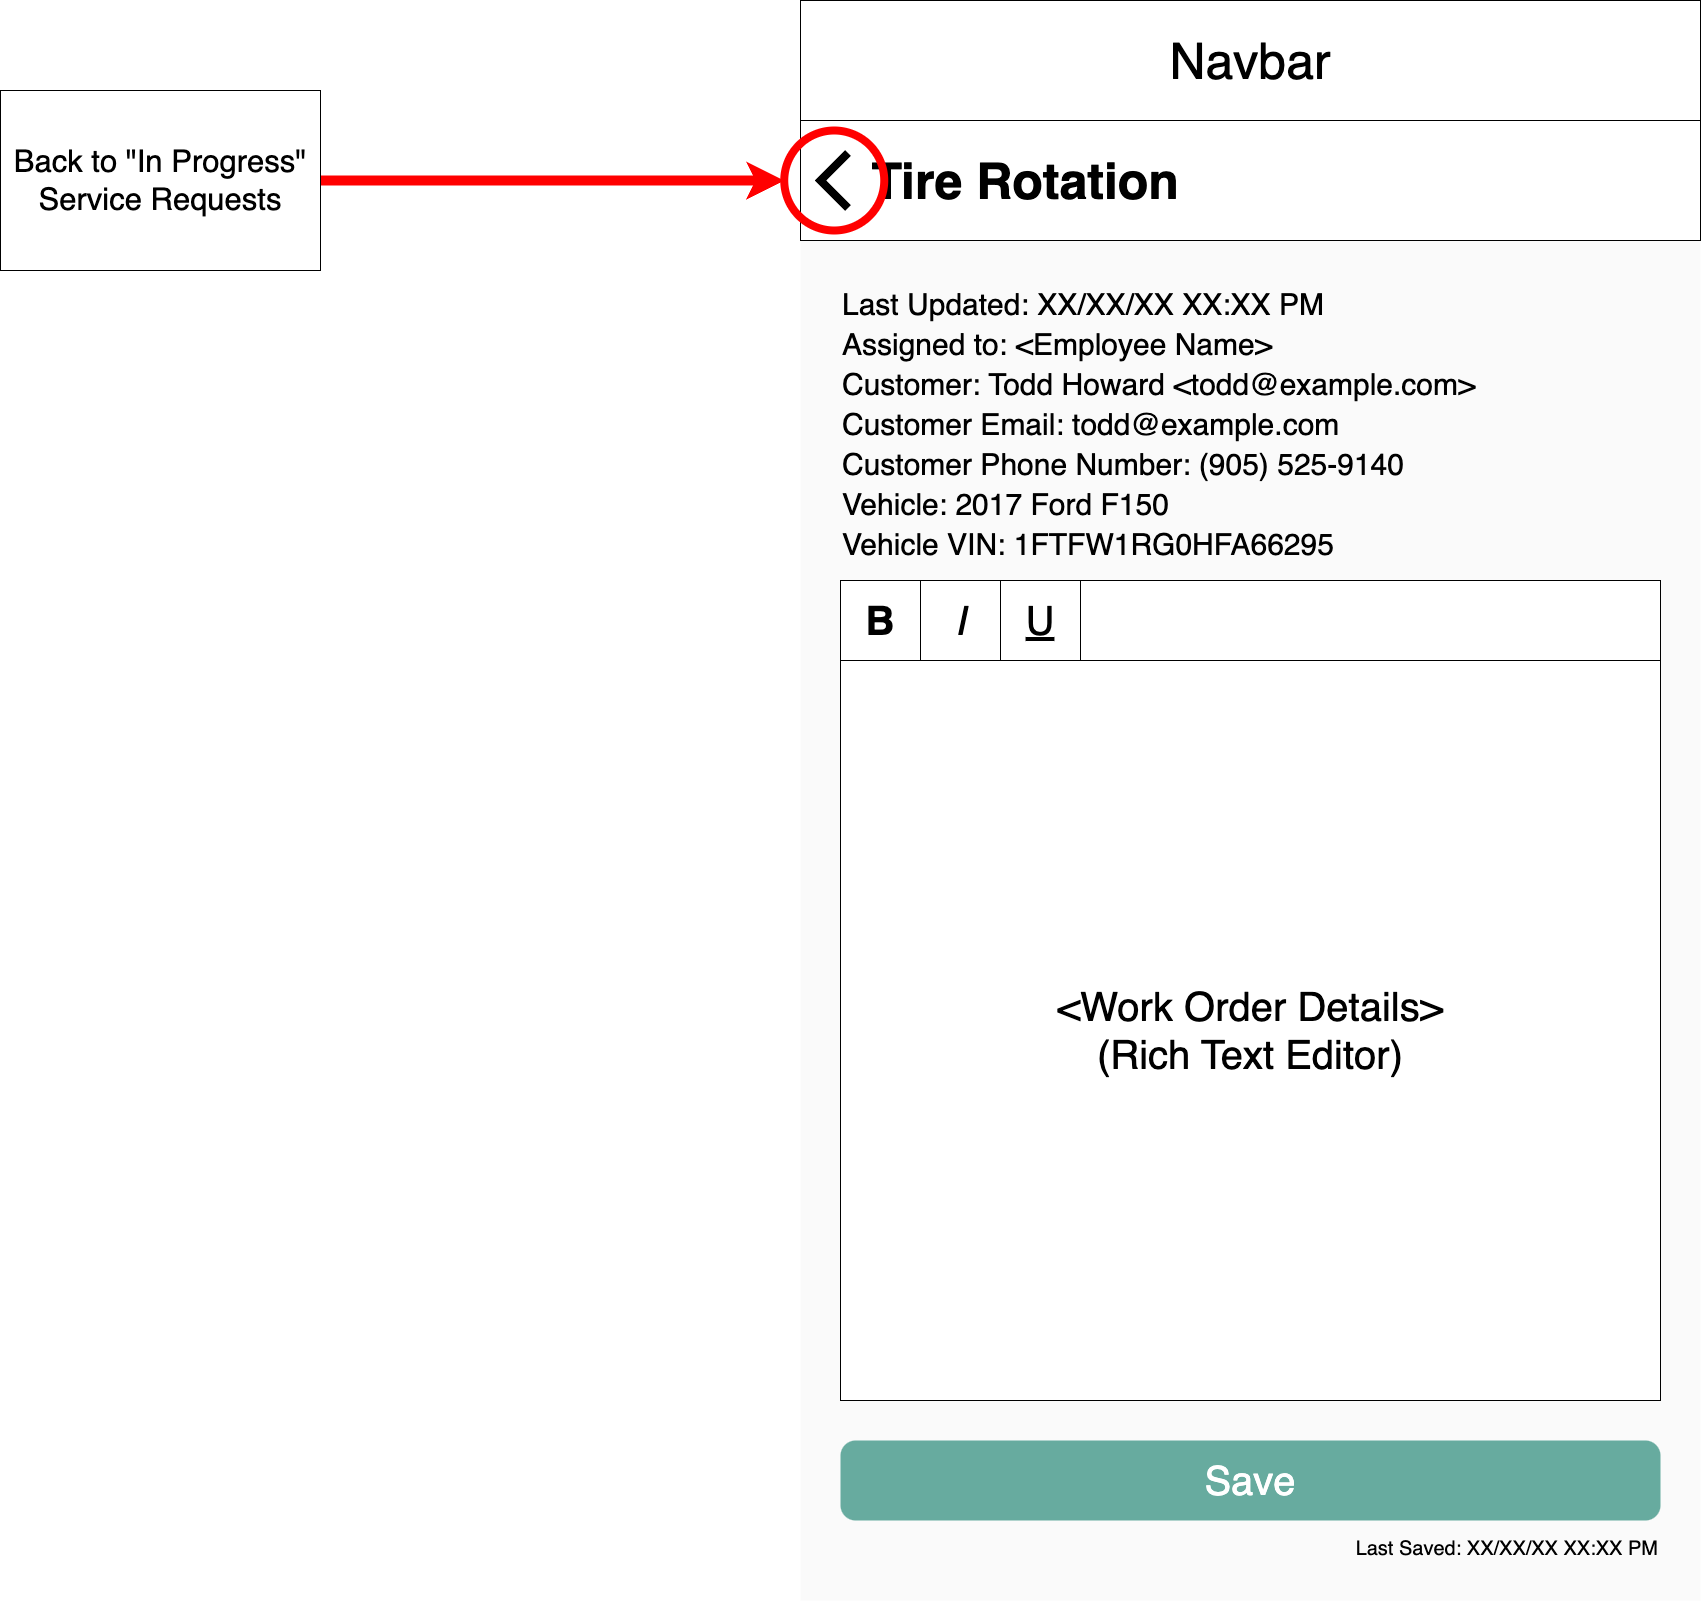
\includegraphics[width=\textwidth]{mockups/Shop Owner-Employee Work Order (Mobile).png}
	\caption{Shop Owner/Employee Dashboard \textemdash{} Service Requests \textemdash{} Work Orders (Mobile)}
\end{figure}

\subsubsection{Service Requests \textemdash{} Completed}

\begin{figure}[H]
	\centering
	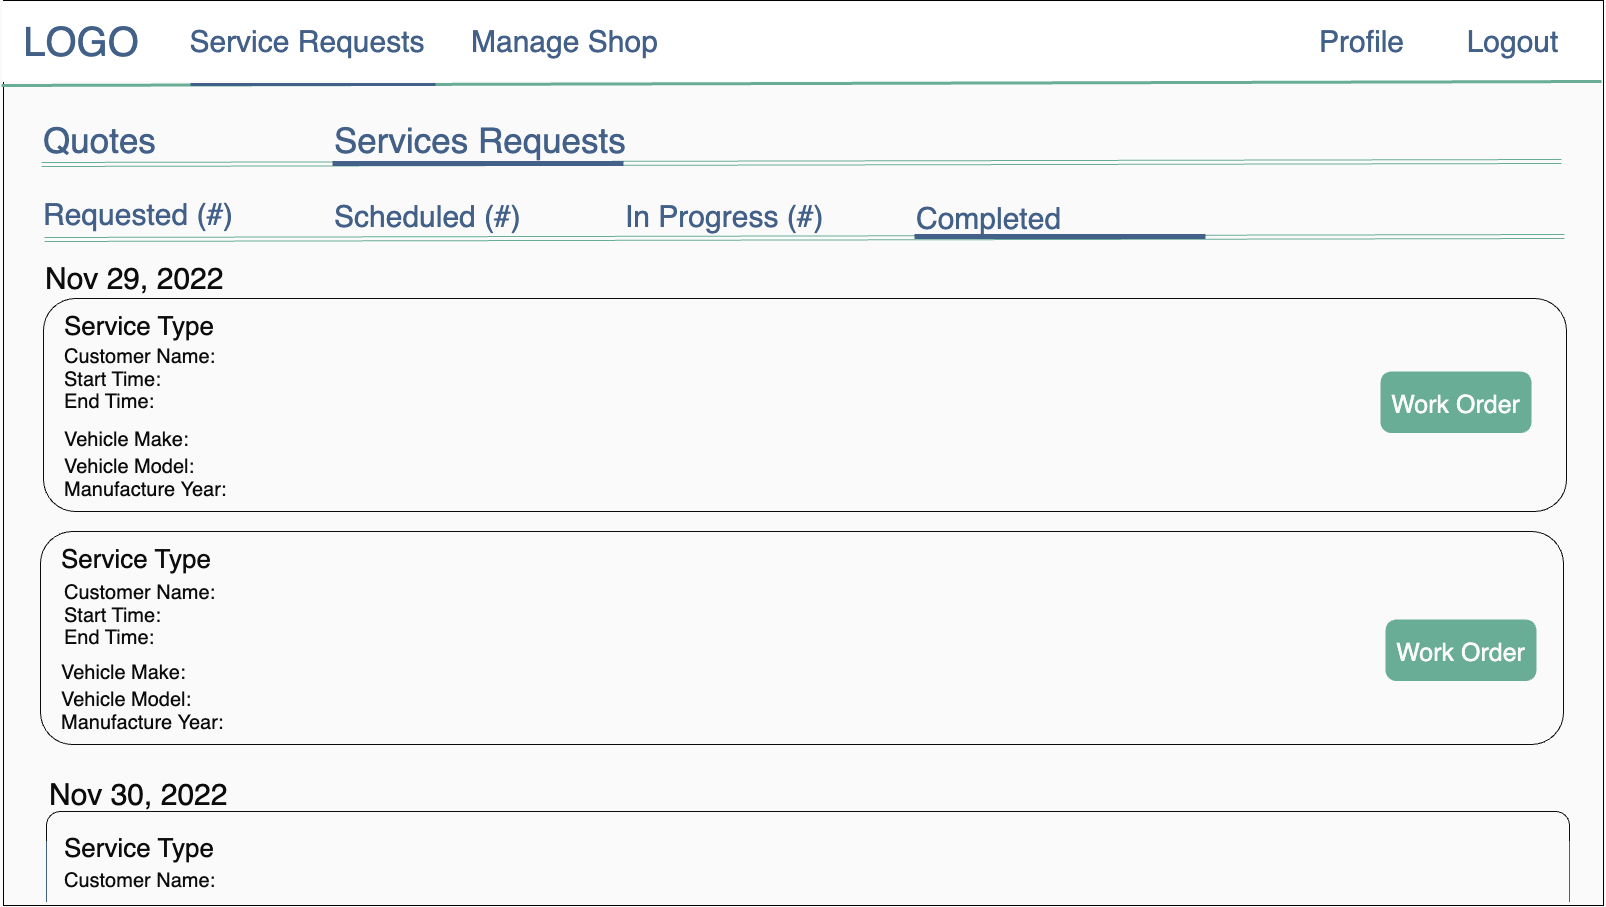
\includegraphics[width=\textwidth]{mockups/Shop Owner Dashboard (Service Requests - Completed) (Desktop).png}
	\caption{Shop Owner/Employee Dashboard \textemdash{} Service \textemdash{} Completed (Desktop)}
\end{figure}

\begin{figure}[H]
	\centering
	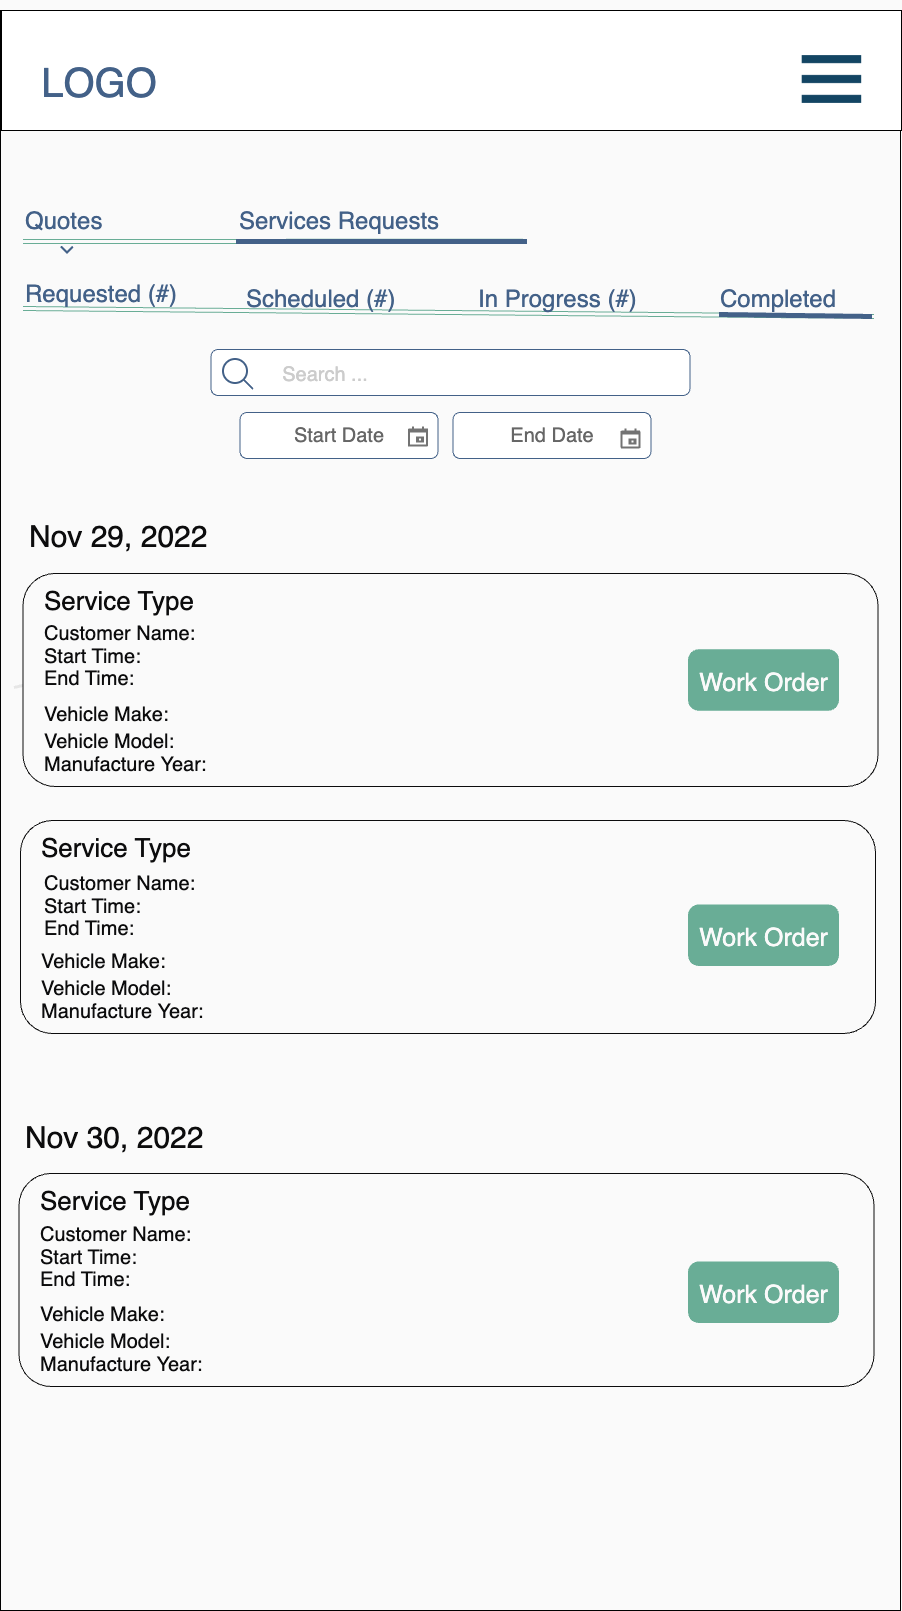
\includegraphics[width=0.5\textwidth]{mockups/Shop Owner Dashboard (Service Requests - Completed) (Mobile).png}
	\caption{Shop Owner/Employee Dashboard \textemdash{} Service \textemdash{} Completed (Mobile)}
\end{figure}

\section{Design of Hardware}
N/A

\section{Design of Electrical Components}
N/A

\section{Design of Communication Protocols}
N/A

\section{Timeline}

\subsection{Module Development}

The development of the modules shall take place over the months of December 2022 and January 2023.
Specific dates, and responsibilities are described in Table \ref{ModuleDevelopmentTimeline}.

\begin{table}[H]
	\caption{Module Development Timeline} \label{ModuleDevelopmentTimeline}
	\begin{tabular}{|p{0.32\textwidth}|p{0.4\textwidth}|p{0.23\textwidth}|}
		\hline
		\textbf{Module Name}       & \textbf{Development Timeline}             & \textbf{Developer(s)}    \\
		\hline
		Database Driver Module     & Dec. 1, 2022 \textemdash{} Jan. 31, 2023  & \makecell[l]{Arkin Modi, \\Joy Xiao,\\Leon So,\\Timothy Choy} \\
		\hline
		Users Module               & Dec. 1, 2022 \textemdash{} Dec. 15, 2022  & \makecell[l]{Arkin Modi, \\Leon So} \\
		\hline
		Employee Management Module & Dec. 15, 2022 \textemdash{} Dec. 22, 2022 & \makecell[l]{Joy Xiao,   \\Leon So} \\
		\hline
		Shop Module                & Dec. 15, 2022 \textemdash{} Dec. 22, 2022 & \makecell[l]{Leon So,    \\Timothy Choy} \\
		\hline
		Quotes Module              & Jan. 1, 2023 \textemdash{} Jan. 8, 2023   & \makecell[l]{Arkin Modi, \\Timothy Choy} \\
		\hline
		Services Module            & Jan. 1, 2023 \textemdash{} Jan. 8, 2023   & \makecell[l]{Arkin Modi, \\Joy Xiao} \\
		\hline
		Appointments Module        & Jan. 15, 2023 \textemdash{} Jan. 22, 2023 & \makecell[l]{Arkin Modi, \\Joy Xiao,\\Timothy Choy} \\
		\hline
		Work Orders Module         & Jan. 15, 2023 \textemdash{} Jan. 24, 2023 & Arkin Modi               \\
		\hline
	\end{tabular}
\end{table}

\subsection{Module Testing}

The testing of the modules shall take place over the months of December 2022 and January 2023. The
tests conducted shall primarily consist of manual testing and have the primary goal of certifying
confidence for the Revision 0 Demonstration. This testing will not include everything described in
the System Verification and Validation Plan. Generally, testing will take place for the week after
development is scheduled to finish. Specific dates, and responsibilities are described in Table
\ref{ModuleTestingTimeline}.

\begin{table}[H]
	\caption{Module Testing Timeline} \label{ModuleTestingTimeline}
	\begin{tabular}{|p{0.32\textwidth}|p{0.4\textwidth}|p{0.23\textwidth}|}
		\hline
		\textbf{Module Name}       & \textbf{Testing Timeline}                 & \textbf{Developer(s)}    \\
		\hline
		Database Driver Module     & Dec. 1, 2022 \textemdash{} Jan. 31, 2023  & \makecell[l]{Arkin Modi, \\Joy Xiao,\\Leon So,\\Timothy Choy} \\
		\hline
		Users Module               & Dec. 15, 2022 \textemdash{} Dec. 22, 2022 & \makecell[l]{Arkin Modi, \\Leon So} \\
		\hline
		Employee Management Module & Dec. 22, 2022 \textemdash{} Dec. 29, 2022 & \makecell[l]{Joy Xiao,   \\Leon So} \\
		\hline
		Shop Module                & Dec. 22, 2022 \textemdash{} Dec. 29, 2022 & \makecell[l]{Leon So,    \\Timothy Choy} \\
		\hline
		Quotes Module              & Jan. 8, 2023 \textemdash{} Jan. 15, 2023  & \makecell[l]{Arkin Modi, \\Timothy Choy} \\
		\hline
		Services Module            & Jan. 8, 2023 \textemdash{} Jan. 15, 2023  & \makecell[l]{Arkin Modi, \\Joy Xiao} \\
		\hline
		Appointments Module        & Jan. 22, 2023 \textemdash{} Jan. 29, 2023 & \makecell[l]{Arkin Modi, \\Joy Xiao,\\Timothy Choy} \\
		\hline
		Work Orders Module         & Jan. 24, 2023 \textemdash{} Jan. 31, 2023 & Arkin Modi               \\
		\hline
	\end{tabular}
\end{table}

% \newpage
% \bibliographystyle {plainnat}
% \bibliography{../../../refs/References}

\newpage

\section{Appendix}

% \subsection{Interface}

% \wss{Include additional information related to the appearance of, and
% 	interaction with, the user interface}

\subsection{Reflection}

The information in this section will be used to evaluate the team members on the graduate attribute
of Problem Analysis and Design. Please answer the following questions:

\begin{enumerate}
	\item What are the limitations of your solution? Put another way, given unlimited resources, what could
	      you do to make the project better? (LO\_ProbSolutions)

	      One of the main limitations on the resources available is the time allotted for this project. This
	      has limited the number of features which we could support for this project.

	      To improve the project, we would propose adding the following features:
	      \begin{itemize}
		      \item Supporting multiple vehicles per customer
		      \item Ability to specify employee skill sets and assign employees to service appointment bookings
		            accordingly
		      \item Adding email notification functionality
		      \item Adding a profile page for employees and customers
		      \item Add analytics dashboards for shop employees and owners
		      \item Ability to delete and remove accounts
		      \item Ability to sign up for employees to sign up to multiple shops
		      \item Ability for shops to view and manage existing customers
		      \item Add a parts entity and inventory management system
		      \item Add a vehicle inspect checklist
	      \end{itemize}

	      In addition, there are some financial constraints on resources made available for the project. If
	      we had unlimited financial resources, we would make the following improvements:
	      \begin{itemize}
		      \item Add a long-lived server to support and manage features that can benefit from being stateful
		      \item Add an email server to support email communication and notifications
	      \end{itemize}

	\item Give a brief overview of other design solutions you considered. What are the benefits and tradeoffs
	      of those other designs compared with the chosen design? From all the potential options, why did you
	      select documented design? (LO\_Explores)

	      Our supervisor provided us with existing mockups for a UI, however, our team took initiative to
	      completely refactor and redesign the application to be more user-friendly. With this, we simplified
	      workflows for the user, to make the user experience more efficient and tailored to fulfill the
	      desired functionality. We also gathered feedback from the project supervisor, and incorporated such
	      feedback into the designs.

	      For the navigation bar, we considered two alternatives for the positioning of the navigation bar.
	      We considered a top and bottom navigation bar for mobile devices. We decided on a top navigation
	      bar, as many of the pages show lots of information and often require scrolling. A top navigation
	      bar is less intrusive when it comes to interfering with scrolling on mobile devices. A top
	      navigation is also more visible and noticeable as the user interacts with the application on their
	      phone.

\end{enumerate}

\end{document}
